\documentclass[12pt]{article}

% --- PREAMBLE ---
% --- XeLaTeX/Font setup ---
\usepackage{fontspec}           % 一定要最先加载
% \setmainfont{Latin Modern Roman}   % TeX Live 通常自带
\usepackage{appendix}
\usepackage{fourier-otf}        % OpenType 版 Fourier 数学字体

% --- 其余宏包 ---
\usepackage[english]{babel}     % 语言
\usepackage{graphicx}            % 插图
\usepackage{subcaption}
\usepackage{xcolor}              % 颜色
\usepackage{geometry}            % 版边
\usepackage[authoryear]{natbib}  % 文献引用
\usepackage{booktabs}            % 表格美化
\usepackage{tabularx}
\usepackage{amsthm}              % 定理环境···
\usepackage{setspace}
\usepackage{tikz}                % 图形绘制
\usepackage{hyperref}            % 超链接
% \usepackage{mathtools} % 提供 \coloneqq, \eqqcolon 等
\usetikzlibrary{positioning,calc,arrows.meta}
\onehalfspacing
% % 定理样式
% \theoremstyle{definition}
% \newtheorem{definition}{Definition}
\providecommand{\coloneqq}{\mathrel{\mathop:}=}
\providecommand{\eqqcolon}{=\mathrel{\mathop:}}

% 页面设置
\geometry{a4paper, margin=1in}
\hypersetup{
  colorlinks,
  citecolor=blue,
}  % For better tables



% Define the "definition" environment style
\theoremstyle{plain}
\newtheorem{definition}{Definition}
\newtheorem{proposition}{Proposition}
\newtheorem{lemma}{Lemma}
\newtheorem{corollary}{Corollary}
\newtheorem{remark}{Remark}

\newcommand{\E}{\mathbb{E}}
\newcommand{\Y}{\mathcal{Y}}
\newcommand{\bbP}{\mathbb{P}}


% --- TITLE BLOCK ---
\title{Default with Policy-Randomness Overestimation}
\author{Chen Gao \thanks{National School of Development, Peking University. Email: \url{chengao0716@gmail.com}. I thank Bo Li and Changhua Yu for thorough guidance. I thank Michael Devereux for helpful advice.}}
\date{{\color{red} [INCOMPLETE AND PRELIMINARY]} \\ \today}

% --- DOCUMENT START ---
\begin{document}

\maketitle

\begin{abstract}
	Why do emerging economies face persistently high borrowing costs despite moderate debt levels? I develop a quantitative sovereign default model where lenders systematically overestimate government policy randomness—policy-randomness overestimation (PRO). This behavioral bias creates a ``PRO wedge'' that pivots bond prices—making debt cheaper near default but more expensive in normal times. Rational sovereigns respond by deleveraging yet paradoxically face higher average spreads and an ``illusion of financial stability'' where volatility falls despite rising risk premiums. Theoretical extensions demonstrate that optimal fiscal policy cannot eliminate allocative distortions from PRO, learning frictions can perpetuate beliefs exhibiting PRO, and strategic communication can partially mitigate these effects. The framework provides a new behavioral foundation for understanding sovereign debt puzzles in emerging markets.
\end{abstract}

\noindent \textbf{Keywords:} Sovereign Default, Behavioral Macroeconomics, Policy-Randomness Overestimation (PRO), Sovereign Spreads, Information Frictions, Argentina, Debt Management.

\noindent \textbf{JEL Codes:} F34, E62, G15, D91.

\clearpage

\section{Introduction}
\label{sec:intro}

Why is sovereign debt in some emerging economies particularly expensive?
Standard models struggle to explain why countries with moderate debt-to-GDP
ratios face persistently high borrowing costs, excess volatility, and puzzling
``decoupling'' from their peers \citep{TomzWright2013,
	MeyerReinhartTrebesch2022}. Argentina exemplifies this puzzle: as documented by
\citep{MorelliMoretti2023}, its borrowing costs often appear divorced from
macroeconomic fundamentals, suggesting a large country-specific risk premium
that defies conventional explanation.

The leading explanation centers on reputation and \textit{information
	frictions} \citep{ColeDowEnglish1995}. In this view, advanced quantitatively by
\citep{MorelliMoretti2023}, lenders are rational but uninformed about a
government's hidden type---whether ``committed'' or ``strategic.'' Policy
missteps like Argentina's inflation misreporting signal a ``bad type,'' causing
persistent reputation downgrades. High spreads reflect the market's efficient
pricing of this revealed information.

This paper explores an alternative \textit{behavioral friction}. What if the
problem is not what lenders do not know, but what they systematically believe
to be true? Departing from rational learning, I posit that lenders suffer from
policy-randomness overestimation (PRO): a second-moment belief distortion about
government policy randomness. While sovereigns face unobserved ``taste
shocks,'' lenders perceive these shocks as larger and more volatile than they
truly are. This ``PRO wedge'' distorts default risk assessment. Events like
Argentina's misreporting signal not just strategic behavior but perceived
policy unpredictability. Markets react to this perceived randomness increase
alongside reputational downgrades, offering a complementary channel rather than
a substitute.

My main contribution embeds this behavioral friction into a quantitative
sovereign default model and traces its macroeconomic consequences. Lenders with
policy-randomness overestimation (PRO) fundamentally alter the borrowing
environment by ``pivoting'' bond price schedules—making debt cheaper near
default but more expensive in safe states. Rational sovereigns respond
optimally by deleveraging yet paradoxically face higher average spreads. The
model generates an “illusion of financial stability” where market volatility
falls despite rising risk premiums. This mechanism is complementary to
reputational learning and can coexist in the data.

\paragraph{Intuition: Deleveraging with Higher Spreads}
The pivoted pricing created by PRO raises spreads precisely where governments
typically borrow and lowers them only near the brink of default. In the normal
borrowing region (future debt $B' < B^*(y)$), PRO magnifies perceived policy
randomness, making lenders demand extra compensation; prices $q$ fall and
spreads $s$ rise even when default risk is low. Near default ($B' > B^*(y)$),
the same belief distortion makes lenders attach more weight to (perceived)
repayment realizations, softening the “doom” and raising prices there. A
rational sovereign facing this pivoted schedule borrows less (deleverages),
which shifts the distribution of choices toward the safe region. Averaging over
states, two forces determine the net effect: (i) a price‑wedge effect—under
PRO, $1/q$ is higher than under rational pricing in the safe region—raises the
average spread; (ii) a composition effect—deleveraging moves weight toward
states with lower baseline spreads—works in the opposite direction. Because the
sovereign spends most of its time in the safe region, the price‑wedge effect
dominates, so average spreads rise even as debt falls. This intuition is
formalized in the paper by a simple two‑term decomposition and local
comparative statics that deliver $\partial q/\partial \theta < 0$ in the safe
region and $\partial q/\partial \theta > 0$ near default.

Three theoretical extensions deepen the analysis. First, even optimal Ramsey
fiscal policy cannot eliminate welfare losses from PRO due to fundamental
allocative inefficiencies from distorted bond pricing. Second, endogenous
belief formation through Bayesian learning with negativity bias shows how
beliefs exhibiting PRO persist and become entrenched. Third, optimal policy
communication demonstrates how governments can strategically choose
transparency levels to partially mitigate the effects of PRO. The analysis
provides a new behavioral foundation for understanding sovereign risk and
persistent debt challenges in emerging economies.

\paragraph{Literature} This paper contributes to the sovereign default literature by proposing a novel
behavioral mechanism to explain persistent empirical puzzles: why do emerging
economies often face high spreads and excess volatility that seem disconnected
from their macroeconomic fundamentals \citep{TomzWright2013,
	MitchenerTrebesch2023}?\footnote{For comprehensive surveys of the sovereign
	debt literature, see \citep{MeyerReinhartTrebesch2022} and \citep{Abbas2019}.}

The dominant paradigm treats default as a purely \textit{strategic decision}
where sovereigns rationally weigh repayment costs against temporary market
exclusion \citep{EatonGersovitz1981, AguiarGopinath2007, Arellano2008}. While
this framework has been successfully extended to incorporate long-term debt and
financial frictions \citep{HatchondoMartinez2009, ChatterjeeEyigungor2012,
	MendozaYue2012},\footnote{Empirical evidence on emerging market business cycles
	and debt restructurings is provided by \citep{NeumeyerPerri2005},
	\citep{CrucesTrebesch2013}, and \citep{ArellanoRamanarayanan2012}.} it
struggles to explain why spreads often remain elevated even when fundamentals
improve.

A second approach emphasizes \textit{reputational concerns}, where past actions
cast long shadows over future borrowing costs \citep{ColeDowEnglish1995,
	Phelan2006}. In this framework, the central question is how lenders learn about
the government's hidden type. While classic models focus on default itself as
the ultimate signal, recent research shows the informational channel is much
broader. For instance, \citep{Fourakis2021} provides quantitative evidence that
investors learn about government types through fiscal and monetary policy
indicators, finding that deficit and inflation surprises significantly affect
perceived default probabilities and that reputation loss often occurs
\textit{before} a default event. This perspective is powerfully exemplified by
the Argentina inflation misreporting episode, rigorously analyzed by
\citep{MorelliMoretti2023}, where a single breach of trust—interpreted as a
credible signal of a ``bad type''—led to years of market exclusion.This rich
view of reputation has been embedded in models that explain how a country can
eventually "graduate" to a high-trust state through a long history of good
behavior \citep{AmadorPhelan2021} and why, in a partial default setting, larger
haircuts must rationally lead to a greater loss of reputation to sustain a
mixed-strategy equilibrium \citep{AmadorPhelan2023}.\footnote{Other important
	contributions to the reputation literature include \citep{ColeKehoe1998} on
	partial versus general reputations, \citep{DErasmo2011} on government
	reputation and debt repayment, \citep{EgorovFabinger2016} on reputational
	effects in sovereign default, and \citep{DovisKirpalani2020,
		DovisKirpalani2021} on reputation in policy design. A key distinction is that
	while reputation models tend to predict (under canonical assumptions) that "bad
	types" default at lower debt thresholds, the mechanism in this paper can imply
	the opposite: PRO lenders may perceive higher default thresholds due to
	overestimated policy randomness.} Yet even this learning-based view assumes
lenders eventually converge to the truth, leaving unexplained why some
sovereign risk premia appear systematically and persistently excessive.

\noindent\textit{Comparative framing.} I view type‑based reputation and PRO as complementary rather than competing channels. Under canonical implementations, reputation models tend to generate monotonic price effects via type revelation, whereas the second‑moment distortion in this paper (PRO) implies a pivoting price schedule. This difference yields distinct, testable predictions for default thresholds, cross‑maturity responses to informational shocks, and spread–cycle comovement. Empirically, both mechanisms may coexist: reputation primarily shifts the perceived mean (type) while PRO inflates the perceived dispersion of policy choices.

A third strand recognizes that market \textit{sentiment itself} can become a
fundamental force. Beginning with \citep{CalvoLeidermanReinhart1996} and
\citep{ColeKehoe2000}, this literature demonstrates how pessimistic
expectations can become self-fulfilling, with modern quantitative
implementations by \citep{GennaioliMartinRossi2014} and
\citep{BocolaDovis2019}.\footnote{Related work explores financial frictions
	\citep{LongstaffPanPedersenSingleton2011}, risk aversion \citep{Lizarazo2013},
	maturity choice \citep{Stangebye2020}, and rational learning about shifts in
	fundamentals, such as the "rare disaster" mechanism in \citep{Paluszynski2023}
	used to explain the slow onset of the European debt crisis.} My paper builds
directly on this insight but asks a deeper question: what if markets
systematically \emph{misperceive} the very nature of sovereign decision-making?

Drawing from behavioral economics, I propose policy-randomness overestimation
(PRO) rooted in well-documented biases like \textit{heuristics and biases}
\citep{TverskyKahneman1974}, \textit{prospect theory}
\citep{KahnemanTversky1979}, and \textit{noise trading}
\citep{DeLongEtAl1990}---can create persistent wedges between sovereign risk
and fundamentals.\footnote{Additional behavioral foundations include investor
	sentiment \citep{BakerWurgler2006}, rare disasters \citep{Gabaix2012},
	disposition effects \citep{ShefrinStatman1985}, crisis psychology
	\citep{Kindleberger1978}, and limits to arbitrage \citep{BrunnermeierNagel2004,
		BarberisThaler2003}.} Crucially, my mechanism differs from existing behavioral
approaches. For instance, models of \textit{ambiguity aversion} based on robust
control theory \citep{GilboaSchmeidler1989, HansenSargent2008} assume that
lenders are uncertain about the true model of macroeconomic fundamentals. This
leads them to price assets based on a "worst-case" scenario, generating an
ambiguity premium that can explain high sovereign spreads
\citep{PouzoPresno2016} and the puzzlingly poor pricing of contingent debt
\citep{RochRoldan2023}. While these models distort the perceived distribution
of \textit{macroeconomic shocks} across all states, my ``PRO wedge''
specifically targets the perceived volatility of the sovereign's \textit{policy
	choices}, creating a distinctive bond-price \textit{pivot}.\footnote{This pivot
	effect differs from both reputation and ambiguity aversion models. While
	reputation models like \citep{AmadorPhelan2021} often generate monotonic price
	effects through type revelation under standard implementations, and
	\citep{Fourakis2021} shows reputation loss \textit{before} default through
	rapid debt accumulation, the mechanism here can produce non-monotonic price
	schedules where debt becomes cheaper near default but more expensive in normal
	times. Similarly, ambiguity models like \citep{RochRoldan2023} explain high
	spreads through a uniform distortion of fundamental shocks, which also differs
	from the pivot mechanism.} And unlike \textit{diagnostic expectations}
\citep{GennaioliShleifer2018, BordaloEtAl2023}, which generate boom-bust cycles
through time-varying news overreaction, my time-invariant bias produces
persistent ``PRO premia,'' counterintuitive deleveraging, and the
``softening-of-doom'' effects that standard formulations may find challenging
to replicate.\footnote{The empirical predictions may differ from those of
	reputation models. While \citep{MorelliMoretti2023} find that misreporting
	episodes increase spreads on all debt instruments, the mechanism here implies
	divergent effects across the debt distribution. Similarly, while
	\citep{AmadorPhelan2023} shows reputation effects strengthen with haircut size,
	the mechanism here implies that PRO effects may weaken as larger haircuts
	reduce the perceived randomness component.}

% --- MOTIVATION ---------------------------------------------------------------
\section{Motivation: Argentina's Inflation--Misreporting Episode}
\label{sec:motivation}

\paragraph{A Puzzle of Persistent Risk}
The recent economic history of Argentina offers a powerful illustration of a
core puzzle in international finance: why do emerging economies often face
borrowing costs that seem disconnected from their macroeconomic fundamentals?
\citep{TomzWright2013, MeyerReinhartTrebesch2022}. Standard models, even those
incorporating reputational dynamics, may not fully account for the persistence
and magnitude of the country-specific risk premium observed in cases like
Argentina, where borrowing costs have often appeared divorced from traditional
measures of repayment capacity \citep{MorelliMoretti2023}. This suggests the
presence of frictions beyond those typically modeled.

\paragraph{The Misreporting Episode}
This puzzle was cast in sharp relief during the inflation misreporting episode
that began in 2007. Following a period of rising inflation, the Argentine
government initiated a direct political intervention in its national statistics
institute, INDEC. Senior technical staff were dismissed and replaced, leading
to an immediate and sustained suppression of the official Consumer Price Index
(CPI) \citep{MorelliMoretti2023}. This official figure diverged starkly from
credible estimates produced by private and provincial sources
\citep{Cavallo2013}. The government's enforcement was aggressive, levying
substantial fines on private consultancies that published their own, more
realistic, data \citep{ReutersFines2013}. The data manipulation grew so
notorious that \textit{The Economist} publicly ceased publishing the official
figures in 2012, and the IMF issued a rare ``declaration of censure'' against
the country \citep{Economist2012, IMFPress2013}.

The financial consequences were profound. As inflation-indexed bonds
constituted a significant portion of public debt, this act amounted to a
\textit{de facto} partial default. The market's reaction was swift and severe.
Argentina's EMBI+ spread, which had been tracking its Latin American peers,
decoupled and widened sharply. Crucially, this repricing was not limited to the
directly affected instruments; it spilled over entirely to its
dollar-denominated sovereign debt. This reaction is paradoxical from a purely
mechanical standpoint: a policy that lowers the real debt burden should have
\textit{decreased} default risk on nominal bonds. The opposite happened,
indicating the event was a pure, and powerful, information shock about the
government's character and future actions.

\begin{figure}[htbp]
	\centering
	\begin{subfigure}[t]{0.49\textwidth}
		\centering
		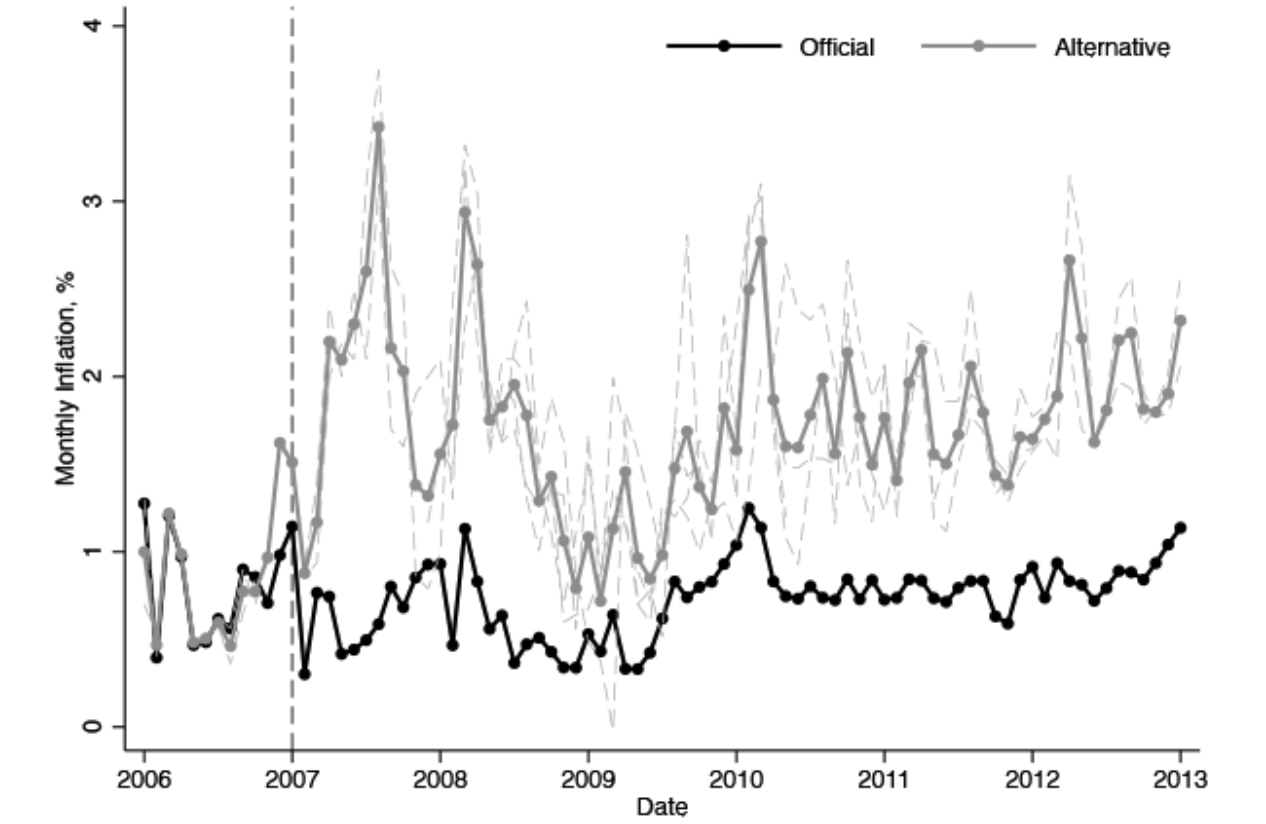
\includegraphics[width=\linewidth]{../../pro-default-model/results/inflation_arg.png}
		\subcaption{Official CPI (black) vs alternative measures (gray).}
		\label{fig:argentina_inflation}
	\end{subfigure}\hfill
	\begin{subfigure}[t]{0.49\textwidth}
		\centering
		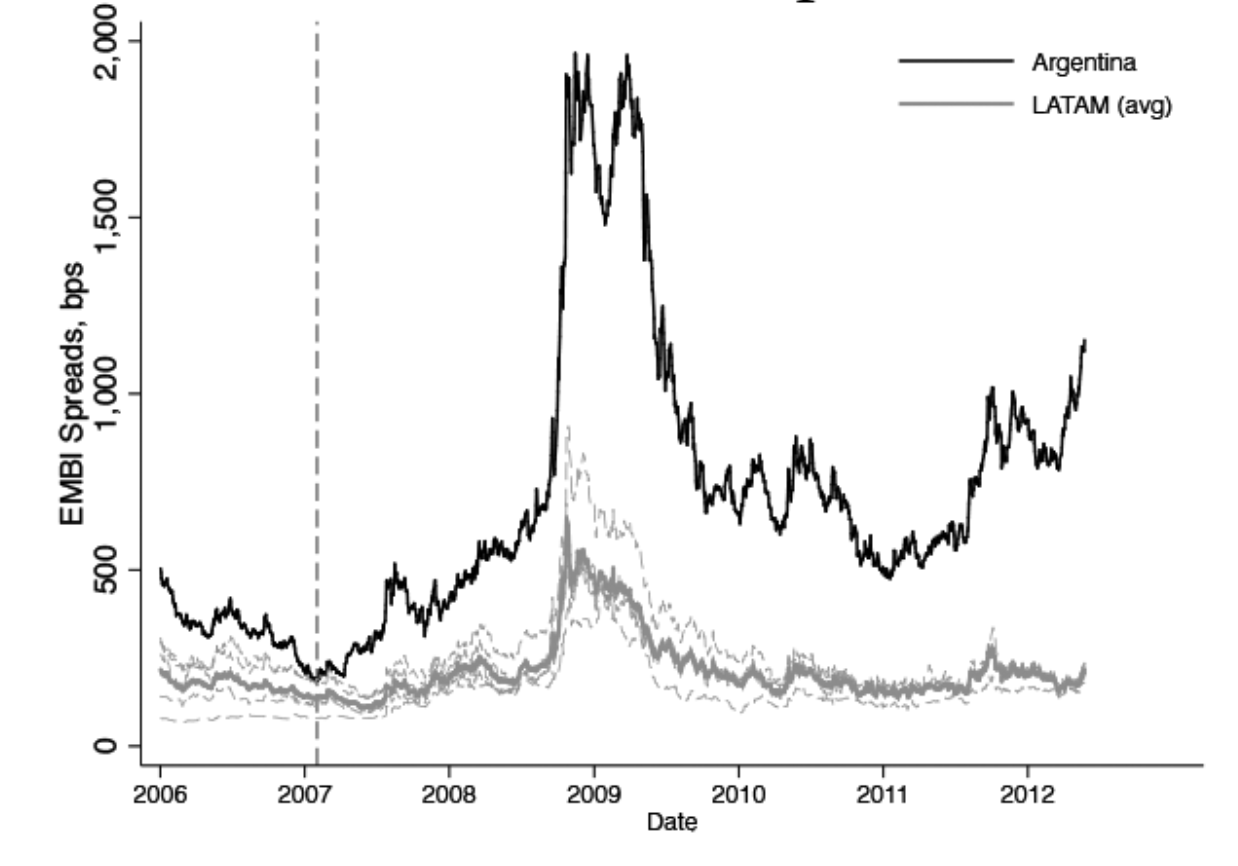
\includegraphics[width=\linewidth]{../../pro-default-model/results/spread_arg.png}
		\subcaption{EMBI+ spreads: Argentina (black) vs other LA (gray).}
		\label{fig:argentina_spread}
	\end{subfigure}
	\caption{Argentina’s misreport of inflation and decoupling of spreads. Panel A shows the monthly official inflation rate announced by the Argentine government (black line) and alternative measures of inflation (gray lines). Panel B shows annualized emerging market bond index spreads for Argentina (black line) and other Latin American countries (gray lines). Vertical lines denote the first month in which the Argentine government underreported the inflation rate. Sources: INDEC (official CPI); private and provincial estimates \citep{Cavallo2013}; J.P. Morgan EMBI+.}
	\label{fig:argentina_spreads}
\end{figure}

\paragraph{Reputational Interpretation and Open Questions}
The conventional explanation, rooted in reputational models
\citep{ColeDowEnglish1995}, interprets this episode as a credible signal of a
"bad type." In this view, advanced by \citep{MorelliMoretti2023}, lenders are
rational but uninformed about a government's hidden commitment to repay. The
misreporting revealed Argentina's government as a ``strategic'' type, leading
to a rational, persistent downgrade of its reputation and, consequently, higher
borrowing costs. While this view is powerful, it leaves lingering questions. If
the market simply learned the government's type, why did the risk premium
appear to contain an additional, seemingly excessive, component? Why did market
sentiment seem to reflect not just a reassessment of character, but a new
apprehension about the government's very predictability? The episode suggests
that the market's reaction was not just to what it learned about the
sovereign's \textit{intent}, but to a perceived increase in its \textit{erratic
	nature}.

\paragraph{Comparative reading} Both channels likely operated during the misreporting episode. A reputational
interpretation views misreporting as a credible signal that raises spreads
broadly by shifting the posterior over types. PRO instead emphasizes a
perceived increase in policy unpredictability (dispersion), which implies a
\emph{pivoting} price schedule: cheaper terms near the brink (due to a
perceived chance of “irrational” repayment) but costlier terms in normal times.
This yields two testable implications: (i) a heterogeneous cross maturity
response—reputation effects tend to lift spreads across instruments, whereas
PRO can produce divergent effects across the debt distribution; and (ii) a
sustained elevation in average spreads even if volatility later declines (an
“illusion of stability”), consistent with a persistent second‑moment bias. See
Table~\ref{tab:prediction_comparison} for a summary of differences under
canonical implementations.

\paragraph{A Behavioral Hypothesis: Policy-Randomness Overestimation (PRO)}
This paper explores an alternative, yet complementary, behavioral friction. I
posit that the problem is not only what lenders do not know, but also what they
systematically overestimate: the randomness in sovereign policy choices
(policy-randomness overestimation, PRO). My core assumption is that lenders
perceive the unobserved shocks driving sovereign policy choices to be larger
and more volatile than they truly are. This ``PRO wedge'' distorts their
assessment of default risk. From this perspective, an event like Argentina's
misreporting is not just a signal of a sovereign's bad character (a strategic
type), but is interpreted as evidence of its erratic nature (high
unpredictability). The market reacts to a perceived increase in policy
randomness, not just a downgrade of its reputation. This overestimation is not
irrational in a colloquial sense; rather, it is a systematic bias in belief
formation, consistent with behavioral findings on how agents process
information under uncertainty \citep{TverskyKahneman1974, BarberisThaler2003}.

\paragraph{A Bridge to the Model}
Motivated by this reinterpretation of the Argentine case, I embed this
behavioral friction into an otherwise standard quantitative sovereign default
model. The subsequent sections will formalize the ``PRO wedge'' and trace its
consequences. I will show that the presence of PRO lenders fundamentally alters
the sovereign's borrowing environment, creating a distinctive "pivoting" of the
bond price schedule. This, in turn, generates a series of counterintuitive but
empirically relevant outcomes: a rational sovereign deleverages yet faces
higher average spreads, and market volatility can fall even as the underlying
risk premium rises, creating an ``illusion of financial stability.'' This
framework provides a new, behaviorally-grounded perspective on the persistent
debt challenges that many emerging economies face.

Roadmap. Section~\ref{sec:model} lays out the environment and recursive
equilibrium; Section~\ref{sec:theory} develops the core comparative statics
(price/spread pivots, default threshold, borrowing, welfare); and
Section~\ref{sec:extensions} embeds policy and information extensions (Ramsey
planning, endogenous beliefs, optimal communication). The appendix collects
proofs and operator analysis.

\section{A Model of Policy-Randomness Overestimation (PRO)}
\label{sec:model}

\subsection{Environment}
Time is discrete and the horizon is infinite, $t = 0, 1, 2, \dots$. The economy
receives a stochastic endowment of a single tradable good, $y_t$. The endowment
process is exogenous and follows a stationary, first-order Markov process,
which is generated by discretizing the following AR(1) process in logarithms:
\begin{equation}
	\ln y' = (1-\rho_y)\mu_y + \rho_y \ln y + \sigma_y \varepsilon', \quad \varepsilon' \sim \mathcal{N}(0, 1).
	\label{eq:endowment}
\end{equation}
The transition probabilities are given by the matrix $\Pi(y, y') = \Pr\{y_{t+1}=y'|y_t=y\}$.

The government can borrow from a large number of competitive, risk-neutral
international lenders who have access to an international risk-free interest
rate $r$. Debt takes the form of long-term bonds. A bond is a claim to a stream
of coupon payments $\kappa$ in every future period, unless the sovereign
defaults. Each period, a fraction $\delta \in (0, 1]$ of outstanding bonds
matures, while the remaining fraction $1-\delta$ carries over to the next
period.

The sovereign government has preferences represented by a standard
time-separable utility function with a discount factor $\beta \in (0, 1)$. The
period utility function is of the CRRA form:
\begin{equation}
	u(c) = \frac{c^{1-\sigma}-1}{1-\sigma},
\end{equation}
which is strictly increasing and concave for $\sigma > 0$.

\subsection{The Sovereign's Problem}
At the beginning of each period $t$, the state is summarized by the current
endowment realization $y \in \mathcal{Y}$ and the stock of outstanding debt
$B$. The sovereign first decides whether to default on its obligations or to
repay. This choice is subject to an idiosyncratic preference shock, often
referred to as a ``taste shock,'' which introduces randomness into the
decision-making process from the perspective of an outside observer.

\paragraph{Taste Shocks}
Let $V^D(y)$ be the deterministic component of the value of defaulting, and
$V^R(y, B)$ be the deterministic component of the value of repaying. The full,
or \textit{ex-post}, value for each choice is the sum of its deterministic part
and a random shock:
\begin{align*}
	\tilde{V}^D(y, \varepsilon_d)    & = V^D(y) + \varepsilon_d    \\
	\tilde{V}^R(y, B, \varepsilon_r) & = V^R(y, B) + \varepsilon_r
\end{align*}
The sovereign observes the shocks $\varepsilon_d$ and $\varepsilon_r$ and chooses the action that yields the highest \textit{ex-post} value. The \textit{ex-ante} value function, from a perspective before the shocks are realized, is the expected maximum of these \textit{ex-post} values:
\begin{equation}
	V(y, B) = \mathbb{E}_{\varepsilon_d, \varepsilon_r} \left[ \max \left\{ \underbrace{V^D(y) + \varepsilon_d}_{\tilde{V}^D(y, \varepsilon_d)}, \underbrace{V^R(y, B) + \varepsilon_r}_{\tilde{V}^R(y, B, \varepsilon_r)} \right\} \right],
\end{equation}
where the expectation is taken over the distribution of the shocks.

Following \citep{DvorkinSancheSaprizaYurdagul2021} and
\citep{MIHALACHEOREEF2024}, I assume that the taste shocks $\varepsilon_d$ and
$\varepsilon_r$ are drawn independently from a Gumbel
distribution.\footnote{The CDF of a Gumbel distribution is given by
	$F(\varepsilon; \mu_L, \eta) = \exp(-\exp(-(\varepsilon-\mu_L)/\eta))$, where
	$\mu_L$ is the location parameter and $\eta > 0$ is the scale parameter. The
	mean of this distribution is $\mu_L + \eta\gamma$, where $\gamma \approx
		0.5772$ is the Euler-Mascheroni constant. For analytical convenience, I choose
	a specific parameterization, Gumbel$(-\eta\gamma, \eta)$, which makes the mean
	of the shocks equal to zero: $\mathbb{E}[\varepsilon_i] = -\eta\gamma +
		\eta\gamma = 0$.} To visualize the distribution of these shocks,
Figure~\ref{fig:gumbel_dist} plots the probability density function (PDF) and
cumulative distribution function (CDF) for the Gumbel distribution, normalized
to have a mean of zero. The scale parameter, $\eta$, is pivotal. It governs the
variance of the taste shocks, given by $\text{Var}(\varepsilon_i) = \frac{\pi^2
		\eta^2}{6}$. A larger $\eta$ signifies greater dispersion in preferences and
introduces more randomness into the sovereign's choice.\footnote{As $\eta \to
		0$, the shocks' influence diminishes, and the model approaches a deterministic
	framework where decisions are based solely on $V^D(y)$ and $V^R(y,B)$.
	Conversely, as $\eta \to \infty$, the deterministic value components become
	negligible, and the choice becomes almost entirely random.} Economically, these
taste shocks can be interpreted as a reduced-form representation of various
unmodeled factors that influence policy, such as political pressures from
domestic constituencies, bureaucratic implementation errors, or the private
information of policymakers. By modeling them as random draws, the framework
acknowledges a degree of inherent unpredictability in government behavior.
\begin{figure}[htbp]
	\centering
	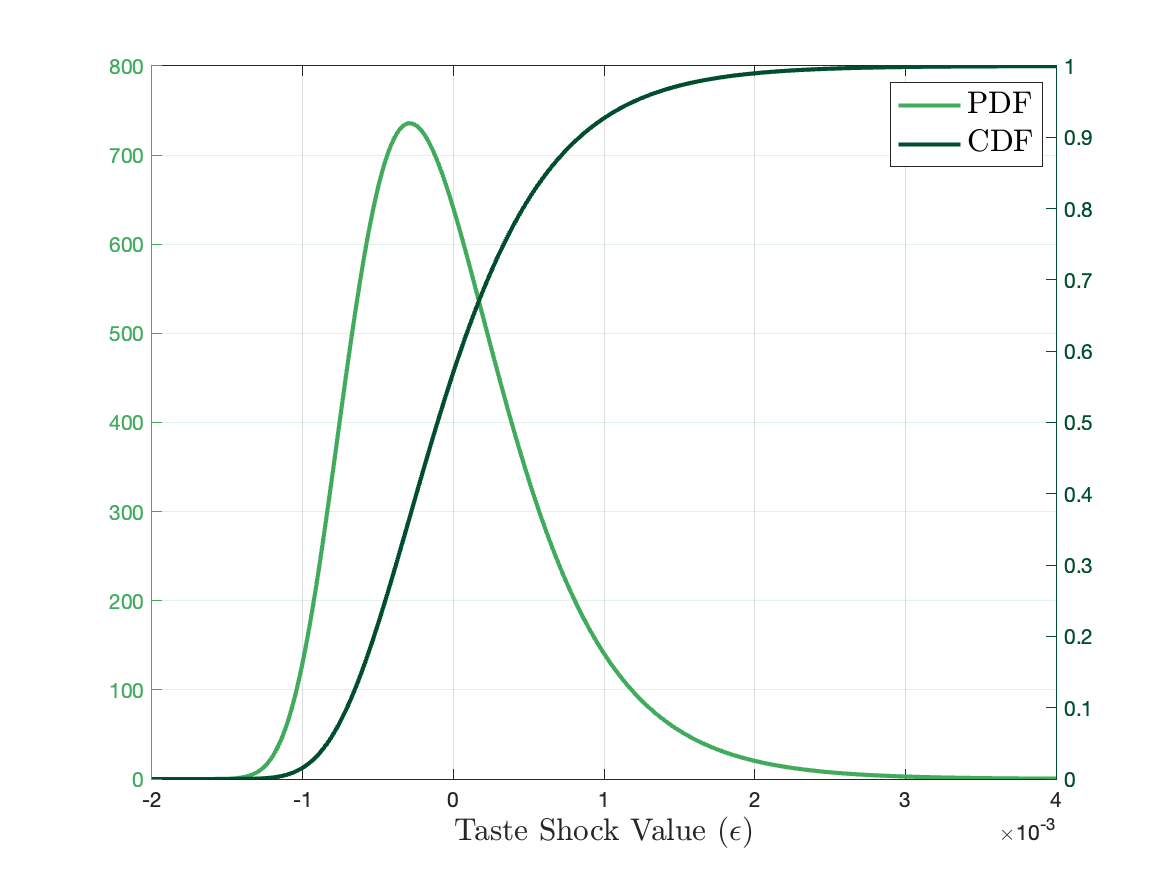
\includegraphics[width=0.6\textwidth]{gumbel_distribution.png}
	\caption{The mean-zero Gumbel distribution ($\eta=5\times 10^{-4}$).}
	\label{fig:gumbel_dist}
	\parbox{\linewidth}{\small\textit{Note:} The Gumbel distribution is used to model the taste shocks in the sovereign's default and borrowing decisions. The scale parameter $\eta$ controls the variance of these shocks. The left $y$ axis is the PDF, the right $y$ axis is the CDF.}
\end{figure}

\paragraph{Ex-Ante Value Function}
The ex-ante value function can be derived using fundamental properties of the
Gumbel distribution. The lemma provided in Appendix \ref{app:gumbel} provides
the closed-form expression for the expected maximum of Gumbel-distributed
random variables, which forms the basis for my analytical solution. First,
applying Lemma~\ref{lem:gumbel_max_expectation} to my setting with $V_1 =
	V^D(y)$ and $V_2 = V^R(y, B)$, the ex-ante value function is:
\begin{equation}\label{eq:V_choice}
	V(y, B) = \mathbb{E}\left[\max\{\tilde{V}^d, \tilde{V}^r\}\right] = \eta \ln\left( \exp\frac{V^D(y)}{\eta} + \exp\frac{V^R(y, B)}{\eta} \right).
\end{equation}

\paragraph{Discrete Choice}
The choice probabilities in my model follow directly from another fundamental
property of the Gumbel distribution. Using Lemma~\ref{lem:gumbel_logit} in
Appendix \ref{app:gumbel}, the probability of default is:
\begin{equation}\label{eq:prd_1}
	\Pr\{d=1 | y, B\} = \frac{\exp\frac{V^D(y)}{\eta}}{\exp\frac{V^D(y)}{\eta} + \exp\frac{V^R(y, B)}{\eta}}.
\end{equation}

\paragraph{Value of Default}
If the sovereign defaults, it is excluded from international credit markets.
During exclusion, it bears an output cost and consumes a fraction of its
endowment, $c = h(y) \le y$, where the output cost function is specified
similar to \citep{ChatterjeeEyigungor2012}:
\begin{equation}
	h(y) = y - \max\{0, \lambda_0 y + \lambda_1 y^2\}.
\end{equation}
In each period of exclusion, there is a constant probability $\gamma \in (0, 1)$ that the country regains market access. Upon re-entry, all past debts are forgiven, so it starts with $B=0$. The value of being in default is therefore:
\begin{equation}
	V^D(y) = u(h(y)) + \beta \mathbb{E}_{y'|y} \left[ \gamma V(y', 0) + (1-\gamma) V^D(y') \right].
	\label{eq:Vd}
\end{equation}

\paragraph{Value of Repayment }
If the sovereign honors its debt, it pays the coupon $\kappa B$ and retains
market access. It can then choose a new level of debt for the next period,
$B'$. This choice is also subject to taste shocks. The \emph{ex-ante} value of
choosing a specific debt level $B'$, given the state $(y, B)$, is:
\begin{equation}
	W(y, B, B') = u\left(y - \kappa B + \left[B' - (1-\delta)B\right] q(y, B')\right) + \beta \mathbb{E}_{y'|y} \left[V(y', B')\right],
\end{equation}
where $q(y, B')$ is the price at which it can issue new bonds. The borrowing choice is subject to i.i.d. Gumbel shocks, denoted by
$\{\varepsilon_{B'}\}$, for each possible debt level $B'$. Each shock is
distributed as Gumbel$(-\rho\gamma, \rho)$. Applying Lemma~\ref{lem:gumbel_multinomial} in Appendix \ref{app:gumbel} with $V_i = W(y, B, B_i)$ and
$\sigma = \rho$, the ex-ante value of repaying is:

\begin{equation}\label{eq:Vr}
	V^R(y, B) = \rho \ln\left( \sum_{B' \in \mathcal{B}} \exp\frac{W(y, B, B')}{\rho} \right),
\end{equation}
where $\mathcal{B}$ is the discrete set of possible debt levels. The probability of choosing a specific level $B'$ is:
\begin{equation}
	\Pr\{B' | y, B\} = \frac{\exp\frac{W(y, B, B')}{\rho}}{\sum_{B_j \in \mathcal{B}}\exp\frac{W(y, B, B_j)}{\rho}}.
\end{equation}
Figure~\ref{fig:borrowing_dist_example} provides a visualization of this
probabilistic borrowing policy. The taste shock framework transforms the choice
of the next debt level, $B'$, from a single deterministic point into a smooth
probability distribution over the entire set of available options,
$\mathcal{B}$. The peak of the distribution corresponds to the most preferred
borrowing choice, but the scale parameter $\rho$ ensures that other, less
optimal choices still have a non-zero probability of being selected. This
feature captures \textit{unobserved heterogeneity} in the sovereign's
decision-making process.\footnote{This probabilistic approach is also crucial
	for the numerical stability of the model, as it replaces the non-differentiable
	``max'' operator with a smooth, analytical expression, which is similar to the idea of \citep{ChatterjeeEyigungor2012}.}

\begin{figure}[h!]
	\centering
	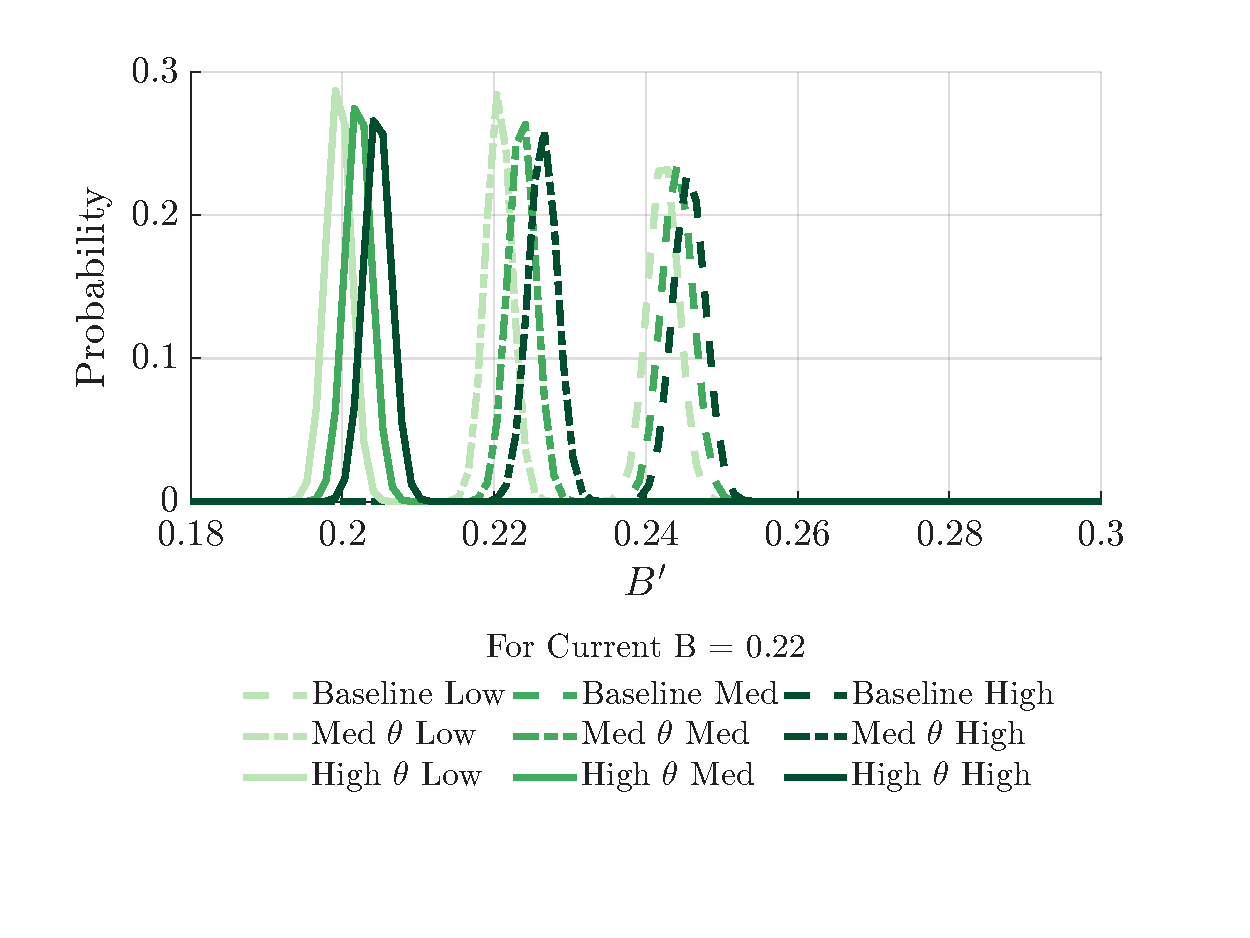
\includegraphics[width=0.6\textwidth]{../../pro-default-model/results/comparison_figure_8.pdf}
	\caption{Example of the Probabilistic Borrowing Policy, $\Pr\{B'|y,B\}$.}
	\label{fig:borrowing_dist_example}
	\parbox{\textwidth}{\small\textit{\textbf{Note:} }The figure illustrates the sovereign's borrowing choice as a probability distribution over possible next-period debt levels ($B'$), given a specific state $(y, B)$. The peak of the distribution represents the most likely choice.}
\end{figure}

\subsection{International Lenders and Bond Pricing}

I depart from the standard model by assuming a \textit{wedge} between the
sovereign's true behavior and lenders' perception of it. Lenders in this model
are competitive and risk-neutral, pricing bonds to make zero expected profit
according to their beliefs. However, their beliefs are systematically biased in
a specific way.

\paragraph{Policy-Randomness Overestimation (PRO)}The key assumption is that lenders perceive the sovereign to be more erratic or
``irrational'' than it truly is. They believe the sovereign's default decision
is governed by a taste shock with a scale parameter $\tilde{\eta} = \theta
	\cdot \eta$, where $\theta \ge 1$. The parameter $\theta$ captures the degree
of \textit{policy-randomness overestimation (PRO)}. This belief distortion is
conceptually distinct from parameter uncertainty or ambiguity aversion. When
$\theta > 1$, lenders act \textit{as if} the government's choices are more
random than they actually are.

Consequently, the lenders' perceived probability of default at a future state
$(y', B')$, which I denote $\tilde{P}(y', B')$, is calculated using this
inflated shock parameter similar to \eqref{eq:prd_1}:
\begin{equation}
	\tilde{P}(y', B') = \frac{\exp\frac{V^D(y')}{\theta\eta}}{\exp\frac{V^D(y')}{\theta\eta}+\exp\frac{V^R(y',B')}{\theta\eta}}.
	\label{eq:plender}
\end{equation}

\paragraph{Bond Price}The equilibrium bond price $q(y, B')$ must satisfy the no-arbitrage condition
based on this overestimation. The price equals the discounted expected payoff,
where the probability of repayment is assessed using $\tilde{P}(y', B')$:
\begin{equation}
	\begin{aligned}
		q(y, B') & = \frac{1}{1+r} \mathbb{E}_{y'|y} \left[ \left(1 - \tilde{P}(y', B') \right) \left( \kappa + (1-\delta) \mathbb{E}_{B''|y',B'} \left[ q(y', B'') \right] \right) \right]            \\
		         & = \frac{1}{1+r} \mathbb{E}_{y'|y} \left[ \left(1 - \tilde{P}(y', B') \right) \left( \kappa + (1-\delta)\sum_{B'' \in \mathcal{B}} \Pr\{B''|y', B'\}\cdot q(y', B'') \right) \right]
	\end{aligned}
	\label{eq:qprice_biased}
\end{equation}
It is important to note that the inner expectation, $\mathbb{E}_{B''|y',B'}$, is taken over the sovereign's \textit{true} borrowing policy, $\Pr\{B''|y', B'\}$, which is governed by the true shock parameter $\rho$. In this framework, lenders correctly understand the sovereign's borrowing behavior but misperceive its propensity to default. This mechanism endogenously generates a credit spread that contains a ``PRO premium'', which reflects the lenders' biased beliefs about the sovereign's stability.

\subsection{Equilibrium}

As is standard in sovereign default literature, the solution concept is a
Recursive Markov Perfect Equilibrium, defined as follows:

\begin{definition}
	\label{def:equilibrium}
	A Recursive Markov Perfect Equilibrium consists of a set of functions: value functions for the sovereign ($V:\mathcal{Y}\times\mathcal{B}\to\mathbb{R}$, $V^R:\mathcal{Y}\times\mathcal{B}\to\mathbb{R}$, $V^D:\mathcal{Y}\to\mathbb{R}$), policy probabilities for its choices ($\Pr\{d=1|\cdot\}, \Pr\{B'|\cdot\}$), and a bond price function ($q:\mathcal{Y}\times\mathcal{B}\to\mathbb{R}$), such that for all states $(y, B)$:
	\begin{enumerate}
		\item \textbf{Sovereign Optimality:} Taking the price function $q$ as given, the sovereign's value functions and policy probabilities solve the dynamic programming problem defined by equations~\eqref{eq:V_choice},~\eqref{eq:Vd}, and~\eqref{eq:Vr}. The choices are governed by the true taste shock parameters $\eta$ and $\rho$.
		\item \textbf{Lender Pricing:} The bond price function $q$ satisfies the zero-expected-profit condition for lenders, as specified in~\eqref{eq:qprice_biased}, which is based on their perceived default probability $\tilde{P}$ from~\eqref{eq:plender}.
	\end{enumerate}
\end{definition}

With the taste shock (logit aggregator) in place, the recursive equilibrium is
well behaved.

\begin{proposition}
	\label{prop:existence_uniqueness}
	Let $\mathcal Y$ and $\mathcal B$ be compact, $u\in C^1$ strictly increasing and concave with $u'$ bounded on the feasible consumption set, and parameters satisfy
	$\beta\in(0,1)$, $r>0$, $\delta\in[0,1)$, $\eta>0$, $\rho>0$, $\kappa>0$.
	Let prices be determined by the pricing operator in~\eqref{eq:pricing_operator} with logistic default rule and repayment/default values as defined in the model, and let the Bellman aggregator be the log-sum-exp with taste-shock scale $\rho$.
	If the slope condition
	\begin{equation}
		\label{eq:SC}
		L_{Jq}\,L_{TV} \;<\; (1-\beta)\Bigl(1-\tfrac{1-\delta}{1+r}\Bigr)
	\end{equation}
	holds (constants defined below), then the Recursive Markov Perfect Equilibrium
	as in Definition~\ref{def:equilibrium} exists and is unique.
\end{proposition}

\begin{proof}
	See Appendix~\ref{app:proof_existence_uniqueness}.
\end{proof}

\paragraph{Unified Operators and Notation}
To keep the subsequent theory tightly anchored to the baseline model, I adopt
an operator view of the same recursive equilibrium. Let $J_\rho$ denote the
sovereign's Bellman aggregator given by the log-sum-exp with borrowing-choice
scale $\rho$, and let $\mathcal T_\theta$ denote the lenders' pricing operator
induced by their perceived default probability with ``policy-randomness
overestimation'' $\theta$. Given the payoff kernel and resale term, the
equilibrium bond price function $q_\theta$ is the unique fixed point of the
pricing operator defined in~\eqref{eq:pricing_operator}. Unless otherwise
noted, all results below are comparative statics or state augmentations
\emph{within this same recursive equilibrium}: primitives, bond structure, and
the Bellman aggregator $J_\rho$ remain unchanged; only the belief parameter
$\theta$ (or information/policy that enters \emph{through} $\mathcal T_\theta$)
differs across the economies I compare.

\section{Theoretical Analysis}
\label{sec:theory}

This section develops comparative statics and extensions within the same
baseline economy defined by Definition~\ref{def:equilibrium} and the pricing
operator in~\eqref{eq:pricing_operator}. Unless stated otherwise, I hold
preferences, technologies, and debt structure fixed, and vary only: (i) the
lenders' belief parameter $\theta$; (ii) the information structure that governs
the evolution of $\theta$ (learning as a slow-moving state); or (iii) planner
instruments that affect resources or the mapping from information to beliefs
while preserving the pricing mechanism. In all cases, equilibrium objects are
unique fixed points of the same operators $J_\rho$ and $\mathcal T_\theta$, so
the results are natural comparative statics of the \emph{baseline} model rather
than separate models.

\paragraph{Toolbox (in brief)}
I repeatedly use three ingredients drawn from the appendix: (i) the pricing
operator $\mathcal T_\theta$ is a contraction and positive, so $(I-\mathcal
	T_\theta)^{-1}$ exists and is positive; (ii) Bellman and pricing operators are
monotone, hence orderings propagate to their fixed points; and (iii)
fixed-point differentiation applies, allowing us to sign $\partial_\theta
	q_\theta$ via an implicit-function argument. Formal statements are collected in
Appendix~\ref{app:operator_analysis}.

Before proceeding to the full quantitative analysis, this section theoretically
unpacks the consequences of the behavioral wedge between the sovereign and its
lenders. I demonstrate how policy-randomness overestimation (PRO, $\theta > 1$)
systematically reshapes the equilibrium, beginning with its most direct impact
on the bond price schedule and tracing the effects through to the sovereign's
policies and ultimate welfare.

\paragraph{Bond Price Pivot}The first and most fundamental consequence of PRO is on the price of debt. The
following comparative-static result is stated \emph{within} the baseline
economy: the only difference across economies is the belief parameter $\theta$
that enters the same pricing operator $\mathcal T_\theta$
in~\eqref{eq:pricing_operator}. PRO does not uniformly depress bond prices;
instead, it causes the price schedule to pivot relative to the rational
benchmark, an effect distinct from the monotonic downward shift one might
associate with reputational deterioration in canonical setups.

\begin{proposition}\label{prop:pivot_concise}
	Consider an economy with PRO lenders ($\theta > 1$) and the baseline economy with rational lenders ($\theta = 1$), both having a small true taste shock parameter $\eta > 0$. Let $q_1(B', y)$ and $q_\theta(B', y)$ be the respective equilibrium bond price functions, each defined as the unique fixed point of the \emph{same} pricing operator $\mathcal T_\theta$ in~\eqref{eq:pricing_operator} evaluated at $\theta=1$ and $\theta>1$, respectively. For a given endowment level $y$, there exists a debt threshold $B^*(y)$ such that the price difference $\Delta q(B', y) \equiv q_\theta(B', y) - q_1(B', y)$ satisfies:
	\begin{itemize}
		\item For levels of future debt $B' < B^*(y)$, $\Delta q(B', y) < 0$ (PRO lenders
		      offer lower prices).
		\item For levels of future debt $B' > B^*(y)$, $\Delta q(B', y) > 0$ (PRO lenders
		      offer higher prices).
	\end{itemize}
\end{proposition}

\begin{proof}
	See Appendix~\ref{app:proof_pivot_concise}.
\end{proof}

The formal proof in Appendix~\ref{app:proof_pivot_concise} proceeds by
comparing default probabilities under the two belief systems. The key insight
is that PRO lenders overestimate default risk in low-debt scenarios (where
fundamentals suggest safety) but underestimate the certainty of default in
high-debt scenarios (where their emphasis on randomness creates perceived
escape possibilities). The pivoting occurs because these two opposing effects
exactly balance at the threshold $B^*(y)$.

Figure~\ref{fig:pivoting_proof} provides a graphical illustration of this
pivoting effect, showing how the bond price schedules for different levels of
PRO levels cross at the threshold $B^*(y)$. The economic intuition behind this
pivoting effect is twofold. For low debt levels ($B<B^*(y)$), where a rational
lender sees default as a remote possibility, a PRO lender prices in a
non-negligible risk of an ``out-of-the-blue'' default driven by the perceived
high variance of taste shocks. This results in a ``PRO premium'' that lowers
the bond price. Conversely, for high debt levels ($B>B^*(y)$), where a rational
lender sees default as a near certainty based on fundamentals, the PRO lender's
view, which emphasizes randomness, makes them less certain of this outcome.

Intuitively, PRO rotates the price schedule so that normal-time borrowing
becomes \emph{more expensive} (a positive ``PRO premium'' at low debt), while
extreme high-debt states become marginally cheaper. Optimal policy moves the
economy away from the region where PRO is favorable and toward the region where
PRO is unfavorable. The average spread must therefore rise.

\begin{figure}[htb]
	\centering
	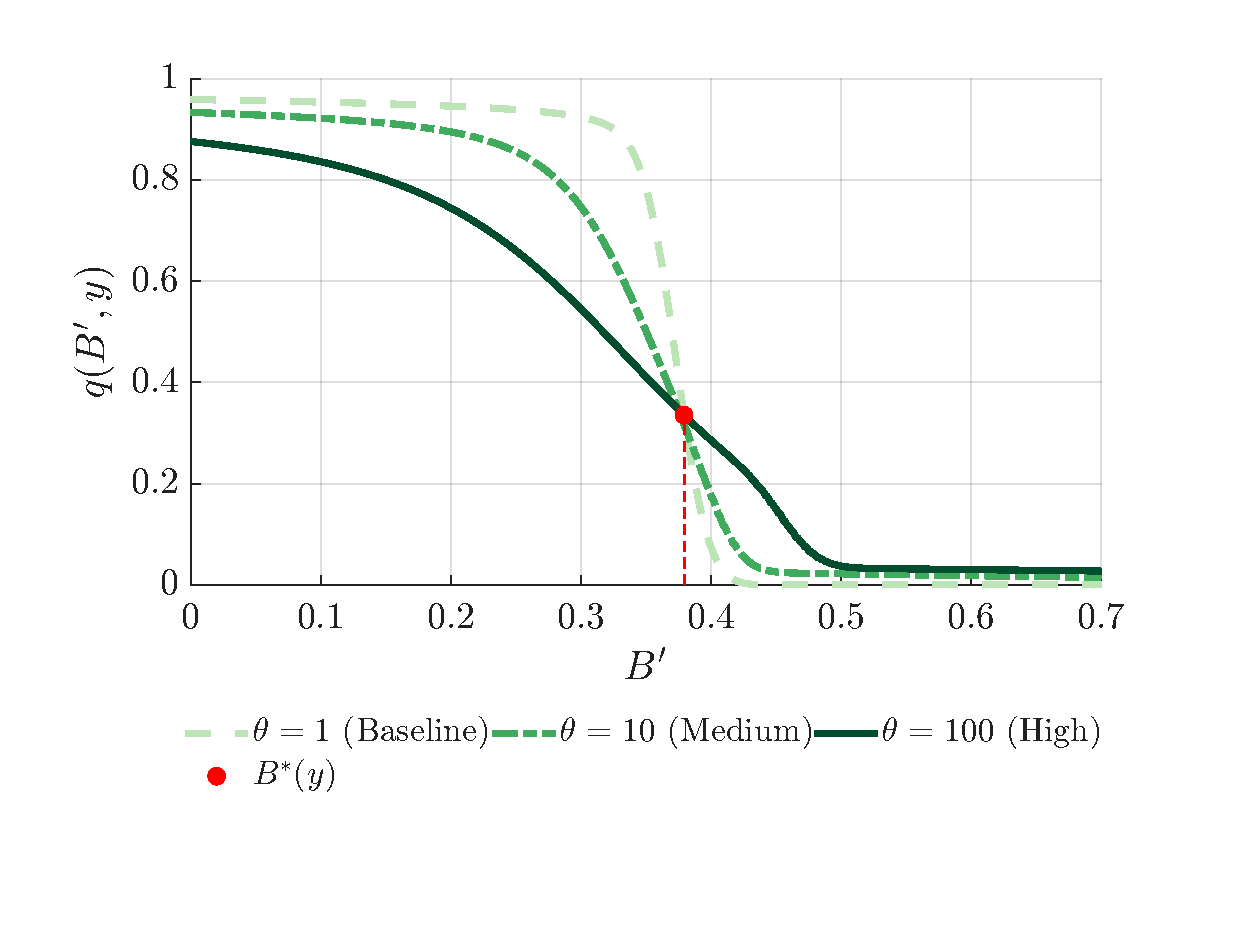
\includegraphics[width=0.8\textwidth]{../../pro-default-model/results/comparison_figure_5.pdf}
	\caption{Pivoting Bond Price Schedules}\label{fig:pivoting_proof}

	\parbox{\textwidth}{\small\textit{\textbf{Note:} }This figure illustrates the pivoting effect described in Proposition~\ref{prop:pivot_concise} for a normal output level. The bond price schedules for three different levels of PRO ($\theta = 1, 10, 100$) cross at the threshold $B^*(y)$ marked by the red dot. To the left of $B^*(y)$, PRO lenders impose a ``PRO premium,'' offering lower prices than rational lenders. To the right of $B^*(y)$, the ``softening of doom'' effect emerges, where PRO lenders offer paradoxically higher prices as they perceive less certainty about default in high-debt scenarios.}
\end{figure}

\paragraph{Pivot Threshold}This pivot point is not static; it responds to the sovereign's economic
condition. The next proposition shows that as the sovereign's fortunes improve,
the pivot point shifts to higher levels of debt.

\begin{proposition}
	\label{prop:monotonicity}
	The debt threshold $B^*(y)$ defined in Proposition~\ref{prop:pivot_concise}, at which the baseline and PRO price schedules cross, is monotonically increasing in the endowment level $y$. That is, $\frac{dB^*(y)}{dy} > 0$. Figure~\ref{fig:monotonicity} illustrates this monotonic relationship.
\end{proposition}

\begin{proof}
	See Appendix~\ref{app:proof_monotonicity}.
\end{proof}
The intuition for this result lies in the differential response of the two markets to good news. A higher income level $y$ improves the sovereign's repayment capacity, shifting both bond price schedules outward. However, the rational market ($q_1$) is more responsive to this positive signal about fundamentals than the PRO market ($q_\theta$), whose pricing remains partially anchored by its skeptical prior about the sovereign's stability. Because the rational price schedule shifts more strongly to the right, its intersection point with the PRO schedule, $B^*(y)$, must also shift to the right. In other words, a stronger economy can sustain more debt before the PRO premium in the low debt region is outweighed by the ``softening of doom'' effect in the high debt region.

\begin{figure}[htb]
	\centering
	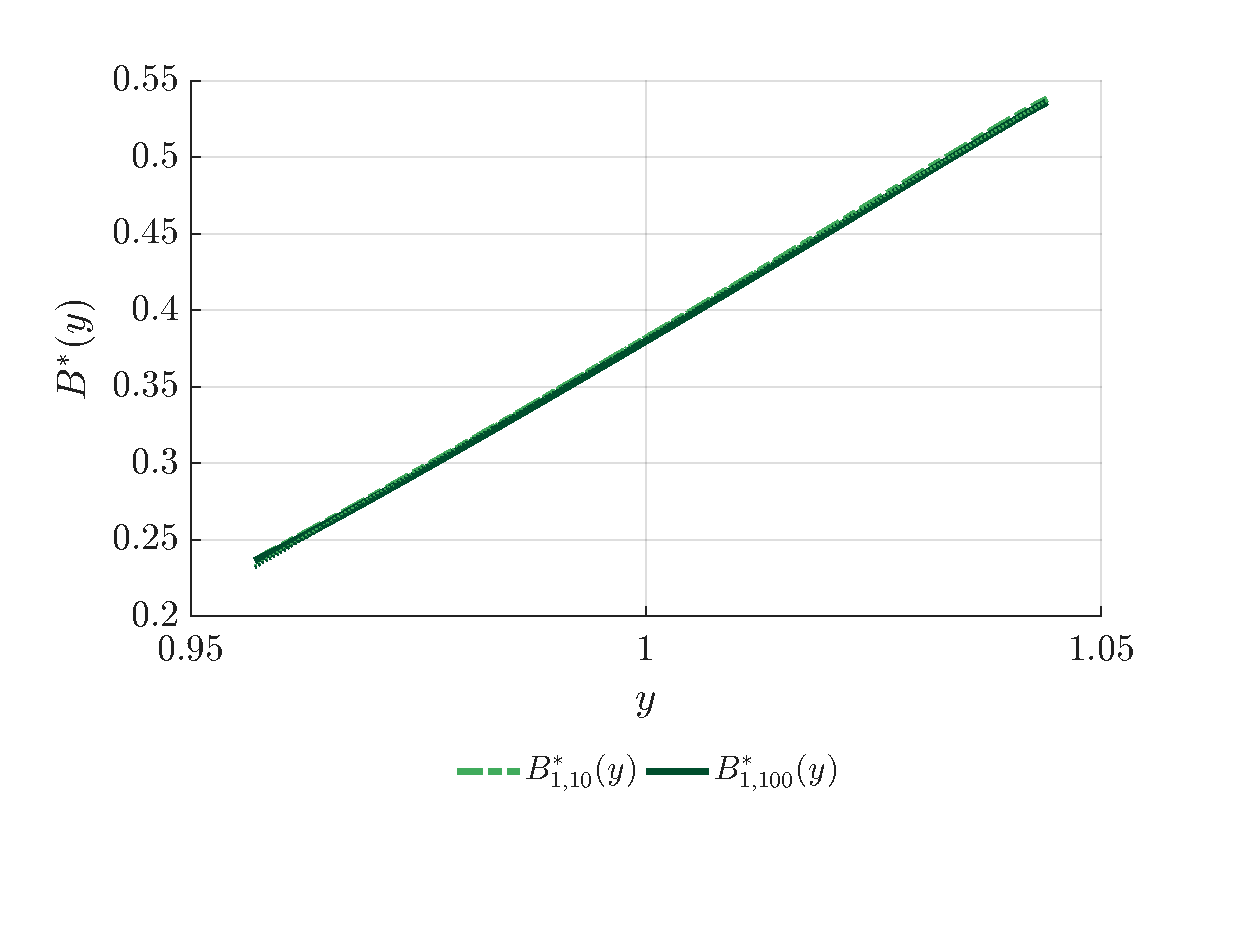
\includegraphics[width=0.8\textwidth]{../../pro-default-model/results/comparison_figure_10.pdf}
	\caption{Monotonicity of Debt Threshold $B^*(y)$}
	\label{fig:monotonicity}
	\parbox{\textwidth}{\small\textit{\textbf{Note:} }This figure illustrates Proposition~\ref{prop:monotonicity} by showing the debt threshold $B^*(y)$ as a function of the endowment level $y$. The threshold represents the debt level at which the baseline ($\theta=1$) and PRO ($\theta>1$) bond price schedules intersect.}
\end{figure}

\paragraph{Spread}
Within the same baseline equilibrium, spreads are an inverse mapping from the
same fixed-point price schedule $q$, so all results below are algebraic
comparative statics of the \emph{same} operators. These results on prices map
directly and inversely to credit spreads. The sovereign credit spread, $s(y,
	B')$, is defined as the yield premium over the risk-free rate, $r$. Given the
bond's price $q(y, B')$, the spread is:
\begin{equation}
	s(y, B') = \frac{\kappa}{q(y, B')} - \delta - r.
	\label{eq:spread_definition}
\end{equation}
This clear, inverse relationship allows the results from Proposition~\ref{prop:pivot_concise} to be restated for credit spreads.

\begin{corollary}
	\label{cor:spread_pivot}
	Let $s_1(B', y)$ and $s_\theta(B', y)$ be the equilibrium credit spreads in the baseline ($\theta=1$) and PRO ($\theta>1$) economies, respectively. The spread difference $\Delta s(B', y) \equiv s_\theta(B', y) - s_1(B', y)$ satisfies the opposite relationship to the price difference at the same threshold $B^*(y)$ defined in Proposition~\ref{prop:pivot_concise}:
	\begin{itemize}
		\item For low levels of future debt $B' < B^*(y)$, $\Delta s(B', y) > 0$.
		\item For high levels of future debt $B' > B^*(y)$, $\Delta s(B', y) < 0$.
	\end{itemize}
\end{corollary}

\begin{proof}
	See Appendix~\ref{app:proof_spread_pivot}.
\end{proof}

\paragraph{Default Threshold}
How does a rational sovereign react to these altered market conditions? The
first area where its behavior changes is at the edge of default. The following
proposition establishes that PRO paradoxically makes the sovereign more
resilient to debt, pushing its default threshold to a higher
level.\footnote{This result differs fundamentally from the negative duration
	effect in \citep{ChatterjeeEyigungor2012}. In their model, longer maturity
	reduces the sovereign's incentive to default because it dilutes existing
	bondholders, creating a debt dilution channel that works through the
	\emph{quantity} of debt issued. In contrast, this mechanism operates through
	lender \emph{beliefs} about the sovereign's decision-making process: PRO
	lenders offer better terms in high-debt states due to their perception of
	greater randomness in sovereign choices, making continued market access more
	valuable and pushing out the default threshold through a behavioral pricing
	channel rather than a debt structure effect.} This contrasts with standard
reputation models, where a sovereign with a worse reputation (i.e., a higher
perceived probability of being a 'strategic' type) would typically be expected
to default at a lower debt level.

In keeping with the unified framework, the objects $V^R_i$ and $q_i$ below are
determined by the \emph{same} Bellman aggregator $J_\rho$ and pricing operator
$\mathcal T_\theta$; only the belief parameter is set to $i\in\{1,\theta\}$.

\begin{proposition}
	\label{prop:threshold}
	Consider economies with PRO lenders ($\theta > 1$) and rational lenders ($\theta = 1$). Let $B^*_{D,i}(y)$ be the sovereign's default threshold for economy $i \in \{1, \theta\}$, defined as the debt level $B$ that satisfies the indifference condition:
	\begin{equation}
		V^R_i(B^*_{D,i}(y),y) = V^D(y) \quad \text{for } i \in \{1, \theta\}.
		\label{eq:default_threshold_definition}
	\end{equation}
	For any given endowment level $y$, the default threshold is higher in the economy with PRO lenders:
	\begin{equation*}
		B^*_{D,\theta}(y) > B^*_{D,1}(y).
	\end{equation*}
\end{proposition}

\begin{proof}
	See Appendix~\ref{app:proof_threshold}.
\end{proof}
The formal proof in Appendix~\ref{app:proof_threshold} proceeds by contradiction, showing that if $B^*_{D,\theta}(y) \leq B^*_{D,1}(y)$, then the "softening of doom" effect from Proposition~\ref{prop:pivot_concise} would make the value of repayment strictly higher under PRO, violating the assumed threshold ordering. The economic mechanism is that PRO lenders offer better prices in high-debt scenarios, increasing the option value of remaining in markets and making sovereigns willing to endure higher debt burdens before defaulting.

The sovereign's decision to default is a trade-off between the immediate
benefit of ceasing payments and the long-term cost of losing market access. The
value of this access depends directly on future borrowing terms. Proposition
\ref{prop:pivot_concise} established the key result that when debt is already
high, PRO lenders offer \textit{better} prices (the``softening of doom''
effect). A rational sovereign in the PRO economy foresees these more favorable
future borrowing terms should it choose to repay. This increases the option
value of repaying and rolling over debt.
\paragraph{Why Average Spreads Rise Despite Deleveraging}
Let $s_i(y,B')$ denote the spread defined in~\eqref{eq:spread_definition} with
price $q_i$ for economy $i\in\{1,\theta\}$, where $q_i$ is the equilibrium bond
price under rational lenders ($i=1$) and PRO lenders ($i=\theta$). Denote by
$\mu_i$ the stationary distribution over non-default states and optimal choices
(including the sovereign's optimal $B'$) in economy $i$. The difference in
average spreads can be written as the decomposition
\begin{equation}\label{eq:spread_decomp}
	\bar s_\theta - \bar s_1 \;=\; \kappa\,\underbrace{\E_{\mu_\theta}\Big[\tfrac{1}{q_\theta}-\tfrac{1}{q_1}\Big]}_{\text{price wedge at PRO weights}}\;\; +\; \kappa\,\underbrace{\Big(\E_{\mu_\theta}\left[\tfrac{1}{q_1}\right] - \E_{\mu_1}\left[\tfrac{1}{q_1}\right]\Big)}_{\text{composition (policy) effect}}\,.
\end{equation}
The pivot result (Proposition~\ref{prop:pivot_concise}) implies that for each $y$ there exists $B^*(y)$ such that $q_\theta(y,B')<q_1(y,B')$ (equivalently, $1/q_\theta>1/q_1$) for $B'<B^*(y)$, and the opposite inequality holds for $B'>B^*(y)$. In the empirically relevant set where new issuance occurs (the primary borrowing region), one typically has $B'<B^*(y)$ and $V^R(y,B')>V^D(y)$.

Two implications follow.
\begin{itemize}
	\item \emph{Local comparative statics.} Differentiating~\eqref{eq:qprice_biased} with respect to $\theta$ yields the linear equation
	      \begin{equation}\label{eq:q_deriv_linear}
		      \big(I - \mathcal T_\theta\big)\,\frac{\partial q_\theta(\cdot)}{\partial\theta}\,(y,B') \;=\; -\frac{1}{1+r}\,\E_{y'|y}\Big[\big(\partial_\theta \tilde P(y',B')\big)\,\Lambda(y',B')\Big],
	      \end{equation}
	      where $\Lambda(y',B')\equiv \kappa + (1-\delta)\sum_{B''\in\mathcal B} \Pr\{B''|y',B'\}\,q_\theta(y',B'')$ and $\mathcal T_\theta$ is the positive linear operator
	      \[\big(\mathcal T_\theta f\big)(y,B') \;=\; \frac{1}{1+r}\,\E_{y'|y}\Big[(1-\tilde P(y',B'))\,(1-\delta)\sum_{B''\in\mathcal B} \Pr\{B''|y',B'\}\, f(y',B'')\Big].\]
	      Because $\|\mathcal T_\theta\|<1$ under discounting and $(1-\delta)<1$,
	      $(I-\mathcal T_\theta)^{-1}$ exists and is positive. Using~\eqref{eq:plender}
	      with $\Delta V(y',B')\equiv V^R(y',B')-V^D(y')$ gives
	      \[\partial_\theta \tilde P(y',B')
		      = \tilde P(y',B')\big(1-\tilde P(y',B')\big)\,\frac{\Delta V(y',B')}{\theta^2\eta}.\]
	      Hence, when $\Delta V(y',B')>0$ (repayment dominates; typically $B'<B^*(y)$),
	      the right-hand side of~\eqref{eq:q_deriv_linear} is negative, implying
	      $\partial q_\theta/\partial\theta<0$, and therefore $\partial
		      s_\theta/\partial\theta>0$ by~\eqref{eq:spread_definition}.
	\item \emph{Average spread dominance.} By~\eqref{eq:spread_decomp}, the first term (price wedge at PRO weights) is strictly positive and \emph{strengthened} by deleveraging, because mass shifts toward $B'<B^*(y)$ where $1/q_\theta - 1/q_1>0$. The second term (composition effect at baseline prices) is weakly negative since $1/q_1$ is lower at smaller $B'$. Under mild regularity (small taste-shock scale $\eta$ and monotone price/borrowing policies), the first term dominates the second, implying $\bar s_\theta>\bar s_1$ even though the sovereign deleverages.
\end{itemize}

\paragraph{Borrowing Policy}
Within the same operator framework, only the belief parameter differs across
economies; the sovereign's choice aggregator $J_\rho$ and the induced price
schedule $q_i$ arise from the same fixed-point problems. While PRO makes the
sovereign more resilient at the brink of crisis, it has the opposite effect on
its day-to-day borrowing. The next proposition shows that a PRO market actively
disciplines the sovereign into adopting a more conservative debt policy.

\begin{proposition}
	\label{prop:deleveraging}
	Consider economies with PRO lenders ($\theta > 1$) and rational lenders ($\theta = 1$). Let $\mathbb{E}_i[B'|y, B]$ be the expected next-period debt level chosen by the sovereign in economy $i \in \{1, \theta\}$ from a given state $(y, B)$. For states $(y, B)$ where the sovereign chooses \textbf{not to default}, the borrowing policy is systematically more conservative under PRO:
	\begin{equation*}
		\mathbb{E}_\theta[B'|y, B] < \mathbb{E}_1[B'|y, B].
	\end{equation*}
\end{proposition}

\begin{proof}
	See Appendix~\ref{app:proof_deleveraging}.
\end{proof}

The formal proof in Appendix~\ref{app:proof_deleveraging} proceeds by comparing
the sovereign's first-order conditions for borrowing under the two price
schedules. The key insight is that lower prices offered by PRO lenders in the
primary borrowing range (as established in
Proposition~\ref{prop:pivot_concise}) reduce the marginal benefit of issuing
new debt. Since the marginal cost of debt remains unchanged, the sovereign
optimally chooses a lower debt level to restore equilibrium between marginal
benefits and costs.

A rational sovereign government reacts optimally to the market prices it faces.
In the region where the sovereign typically wants to borrow, PRO lenders offer
lower prices for new debt. A lower bond price is a direct signal that borrowing
has become more expensive. Faced with a higher cost of capital, the sovereign's
optimal response is to borrow less. The PRO market, through its pricing,
effectively ``disciplines'' the sovereign, forcing it to deleverage and adopt a
more conservative fiscal policy than it would if it faced a rational market.
This endogenous deleveraging is a key mechanism through which market beliefs
shape real economic outcomes.

\paragraph{Welfare}
The final step in the theoretical analysis is to evaluate the net effect of
these changes on the sovereign's well-being. The final proposition demonstrates
that the consequences of PRO translate directly into a welfare loss for the
sovereign.

\begin{proposition}
	\label{prop:welfare}
	Let $V_i(y,B)$ denote the sovereign's ex-ante equilibrium value function in economy $i\in\{1,\theta\}$, where $\theta>1$ indexes PRO lenders and $\theta=1$ rational lenders.
	Suppose that for the given state $(y,B)$ the sovereign has market access and the baseline optimal choice $B'_1(y,B)$ lies on the ``risky'' side of the price pivot $B^*(y)$, i.e. $B'_1(y,B)\ge B^*(y)$.
	Then equilibrium welfare is strictly lower under PRO lenders:
	\[
		V_\theta(y,B) \;<\; V_1(y,B).
	\]
	If $B'_1(y,B) \le B^*(y)$ (``safe'' side), the weak inequality $V_\theta(y,B)
		\le V_1(y,B)$ holds.
\end{proposition}

\begin{proof}
	See Appendix~\ref{app:proof_welfare}.
\end{proof}
The formal proof in Appendix~\ref{app:proof_welfare} proceeds using operator theory to show that pricing under PRO systematically reduces the sovereign's choice-specific value for all borrowing decisions. The key insight is that welfare loss stems directly from a tighter budget constraint: for any given amount of new borrowing, the sovereign receives fewer resources today under PRO lenders. While sovereigns adjust policies optimally (borrowing less, tolerating higher debt before default), they cannot fully escape the welfare loss from transacting with distorted markets.

The sovereign's welfare is fundamentally derived from its ability to use
international financial markets to smooth consumption over time. The terms of
this access are dictated by the bond price schedule, $q(y,B')$, which can be
seen as the price of intertemporal trade. PRO, by inducing a lower $q$ in the
low debt ($B' < B^*(y)$) region, effectively acts as a tax on the sovereign's
ability to conduct this trade. For any given amount of borrowing, the sovereign
receives fewer resources today, which directly curtails its consumption
possibilities and lowers utility. While the sovereign optimally adjusts its
policies in response—by borrowing less and tolerating more debt before
default—it cannot fully escape the welfare loss imposed by being forced to
transact with a paranoid market. The ``benefit'' of better prices in the high
debt ($B' > B^*(y)$) region is an option too remote and uncertain to compensate
for the welfare losses incurred due to worse prices in the normal course of
borrowing.

\paragraph{The Causal Chain of PRO}
The theoretical results presented above follow a clear causal chain originating
from the single shock of PRO ($\theta > 1$). This shift in beliefs first and
foremost reshapes the market environment by altering the bond price schedule,
causing it to \textit{pivot} as established in Proposition
\ref{prop:pivot_concise}. The inverse pivoting of the credit spread schedule,
described in Corollary~\ref{cor:spread_pivot}, is an immediate algebraic
consequence. In response to this new pricing reality, the rational sovereign
optimally adjusts its policies. It leverages the ``softening of doom'' effect
in the high debt region—where PRO lenders offer paradoxically better prices—to
endure a greater debt burden before defaulting (Proposition
\ref{prop:threshold}). Simultaneously, it reacts to the ``PRO premium'' in the
primary borrowing region by systematically deleveraging and adopting a more
conservative debt policy (Proposition~\ref{prop:deleveraging}). This set of
constrained-optimal policy adjustments, however, cannot fully overcome the
handicap of transacting with a paranoid market, culminating in awelfare loss
for the sovereign (Proposition~\ref{prop:welfare}).\footnote{This welfare loss
	is fundamental and cannot be eliminated even by optimal fiscal policy.
	Section~\ref{sec:ramsey} develops a formal Ramsey planning extension
	(Proposition~\ref{prop:ramsey_welfare}) showing that the PRO-induced distortion
	of intertemporal prices creates deadweight losses that persist beyond what
	lump-sum transfers can correct.}

Figure~\ref{fig:causal_chain} illustrates this causal mechanism, showing how a
single behavioral friction propagates through the economy's equilibrium
relationships.
\begin{figure}[htb]
	\centering
	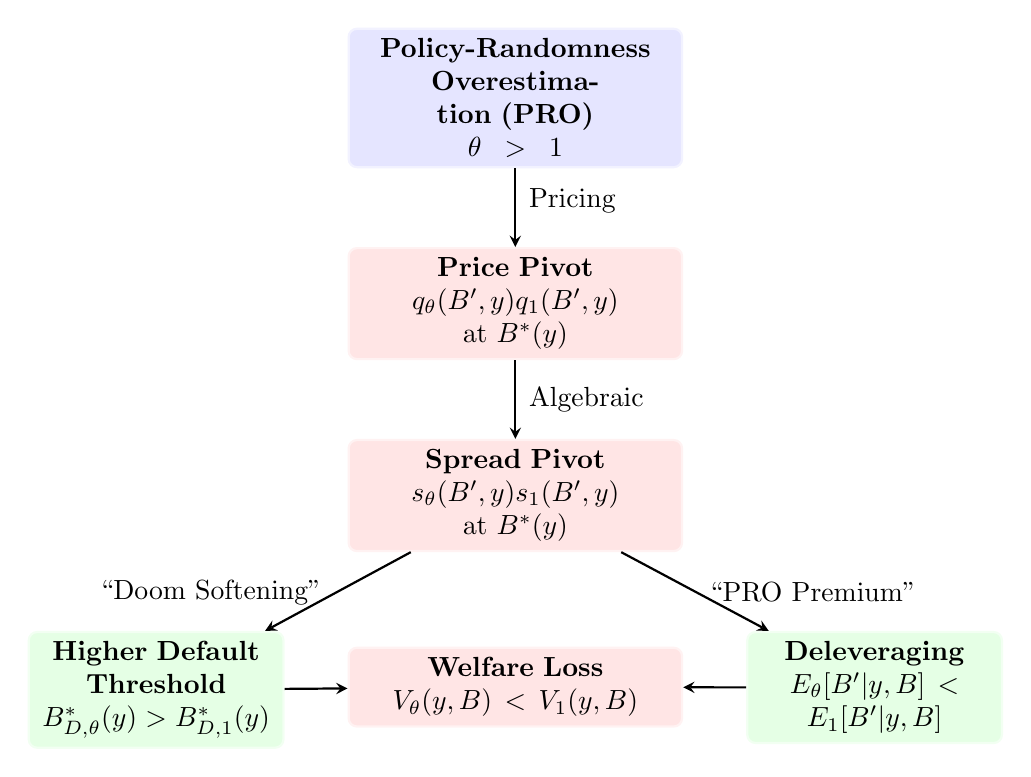
\begin{tikzpicture}[
			node distance=1cm and 1.5cm,
			every node/.style={text centered, minimum height=0.8cm},
			box/.style={rectangle, draw=blue!5, thick, fill=blue!10,text width=4cm, minimum height=1cm, rounded corners=3pt},
			arrow/.style={->, thick, >=stealth},
			effect/.style={rectangle, draw=red!5, thick, fill=red!10, text width=4cm, minimum height=1cm, rounded corners=3pt},
			outcome/.style={rectangle, draw=green!5, thick, fill=green!10, text width=3cm, minimum height=1cm, rounded corners=3pt}
		]

		% Initial shock
		\node[box] (shock) {\textbf{Policy‑Randomness Overestimation (PRO)} \\ $\theta > 1$};

		% Market effects
		\node[effect, below=of shock] (pivot) {\textbf{Price Pivot} \\ $q_\theta(B',y) \gtrless q_1(B',y)$ \\ at $B^*(y)$};

		\node[effect, below=of pivot] (spread) {\textbf{Spread Pivot} \\ $s_\theta(B',y) \lessgtr s_1(B',y)$ \\ at $B^*(y)$};

		% Policy responses (left and right)
		\node[outcome, below left=1cm and 0.8cm of spread] (threshold) {\textbf{Higher Default} \\ \textbf{Threshold} \\ $B^*_{D,\theta}(y) > B^*_{D,1}(y)$};

		\node[outcome, below right=1cm and 0.8cm of spread] (deleverage) {\textbf{Deleveraging} \\ $\mathbb{E}_\theta[B'|y,B] <$ \\ $\mathbb{E}_1[B'|y,B]$};

		% Final outcome
		\node[effect, below=1.2cm of spread] (welfare) {\textbf{Welfare Loss} \\ $V_\theta(y,B) < V_1(y,B)$};

		% Arrows
		\draw[arrow] (shock) -- (pivot);
		\draw[arrow] (pivot) -- (spread);
		\draw[arrow] (spread) -- (threshold);
		\draw[arrow] (spread) -- (deleverage);
		\draw[arrow] (threshold) -- (welfare);
		\draw[arrow] (deleverage) -- (welfare);

		% Labels on arrows
		\node[right=0.05cm] at ($(shock)!0.5!(pivot)$) {Pricing};
		\node[right=0.05cm] at ($(pivot)!0.5!(spread)$) {Algebraic};
		\node[left=0.05cm] at ($(spread)!0.5!(threshold)$) {``Doom Softening''};
		\node[right=0.05cm] at ($(spread)!0.5!(deleverage)$) {``PRO Premium''};

	\end{tikzpicture}
	\caption{The Causal Chain of PRO}
	\label{fig:causal_chain}
	\parbox{\linewidth}{\small\textit{Note:} This diagram illustrates how a single behavioral friction ($\theta > 1$) propagates through the economy. PRO first alters market pricing, creating a pivoting bond price schedule. The sovereign optimally responds to this new environment, but cannot fully escape the welfare costs of dealing with biased lenders.}
\end{figure}
To crystallize the novel contributions of this behavioral channel, Table
\ref{tab:prediction_comparison} explicitly contrasts the key predictions of the
PRO model with those of a standard reputation model.

\begin{table}[h!]
	\centering
	\caption{Comparative Predictions: Reputation and PRO}
	\label{tab:prediction_comparison}
	\begin{tabularx}{\textwidth}{@{}lXX@{}}
		\toprule
		Prediction Dimension                       & Reputation (canonical) \citep{ColeDowEnglish1995, MorelliMoretti2023} & Policy-Randomness Overestimation (PRO)                    \\ \midrule
		Price Curve, $q$                           & Tends to be \textit{lower} (monotonic in canonical setups)            & \textit{Pivots} around baseline ($q_1$)                   \\
		Default Threshold, $B^*_D$                 & Tends to be \textit{lower}                                            & \textit{Higher}: $B^*_{D,\theta} > B^*_{D,1}$             \\
		Expected Borrowing, $\mathbb{E}[B']$       & Often \textit{lower} (constraint-driven)                              & \textit{Lower} (price-driven in this model)               \\
		Average Spread, $\mathbb{E}[s]$            & \textit{Higher}                                                       & \textit{Higher}                                           \\
		Cross-maturity response after misreporting & Tends to increase across instruments                                  & Divergent across debt distribution (pivot-consistent)     \\
		Haircut-size effect on spreads             & Strengthens with larger haircuts \citep{AmadorPhelan2023}             & May weaken if larger haircuts reduce perceived randomness \\\bottomrule
	\end{tabularx}
	\parbox{\linewidth}{\small\textit{Note:} This table compares predictions under canonical implementations of reputation models with the behavioral mechanism in this paper. The PRO column reflects this model's implementation assumptions.}
\end{table}

\section{Quantitative Analysis}
\label{sec:quant}

In this section, I describe the quantitative implementation of the model. I
first outline the calibration of the model parameters and the numerical
strategy used to solve for the equilibrium. Then, I present the business cycle
properties generated by the baseline model and show that it successfully
replicates key features of emerging market economies.

\subsection{Calibration and Numerical Solution}

\paragraph{Calibration}
The model is calibrated at a quarterly frequency. The parameter values are
chosen to be consistent with the sovereign default literature and to broadly
match the macroeconomic features of a typical emerging economy, such as
Argentina. The parameters are summarized in Table~\ref{tab:calibration}.

The preference and endowment parameters are standard. The risk aversion
coefficient $\sigma$ is set to 2. The discount factor $\beta$ is set to 0.9775,
implying an annual real interest rate of approximately 9.5\% when combined with
the model's growth, which is a common value for emerging economies. The
logarithmic endowment process is modeled as an AR (1) with a persistence of
$\rho_y=0.95$ and an innovation standard deviation of $\sigma_y=0.005$.

The debt structure parameters are set to achieve a target Macaulay duration of
5 years (20 quarters) for a risk-free bond, which implies a quarterly principal
decay rate of $\delta=0.04$. The coupon rate $\kappa$ is set to equal
$\delta+r$ so that the price of a risk-free bond is normalized to one. The
probability of re-entering credit markets after a default, $\gamma$, is set to
0.125, implying an average exclusion period of 2 years (8 quarters). The output
cost of default, governed by $\lambda_0$ and $\lambda_1$, is specified to be
nonlinear, consistent with the findings of
\citep{ChatterjeeEyigungor2012}.\footnote{The specific values are $\lambda_0 =
		-0.48$ and $\lambda_1 = 0.525$, calibrated to match the severity and shape of
	output losses observed in historical default episodes.}

The scale parameters of the Gumbel taste shocks, $\eta$ and $\rho$, are set to
small values to ensure that decisions are primarily driven by economic
fundamentals, while still ensuring the stability and tractability of the
numerical solution.\footnote{Specifically, $\eta = 5 \times 10^{-4}$ for
	default decisions and $\rho = 1 \times 10^{-5}$ for borrowing decisions. These
	small values maintain the primacy of economic fundamentals while providing
	computational tractability through the log-sum-exp formulation.}

\begin{table}[h!]
	\centering
	\caption{Baseline Calibration (Quarterly)}
	\label{tab:calibration}
	\begin{tabular}{@{}lll@{}}
		\toprule
		Parameter              & Value              & Description                                  \\ \midrule
		\multicolumn{3}{l}{\textit{Preferences and Endowments}}                                    \\
		$\sigma$               & 2.0                & CRRA coefficient of relative risk aversion   \\
		$\beta$                & 0.9775             & Sovereign's discount factor                  \\
		$\rho_y$               & 0.95               & Persistence of log endowment AR(1)           \\
		$\sigma_y$             & 0.005              & Std. dev. of endowment innovations           \\
		\multicolumn{3}{l}{\textit{Debt and Default}}                                              \\
		$r$                    & 0.01               & Quarterly risk-free interest rate (4\% ann.) \\
		$\delta$               & 0.04               & Principal decay rate (for 5-year duration)   \\
		$\kappa$               & 0.05               & Coupon rate ($\delta+r$)                     \\
		$\gamma$               & 0.125              & Re-entry probability (avg. 2-year exclusion) \\
		$\lambda_0, \lambda_1$ & -0.48, 0.525       & Output cost function parameters              \\
		\multicolumn{3}{l}{\textit{Computational Parameters}}                                      \\
		$\eta$                 & $5 \times 10^{-4}$ & Scale of default taste shock                 \\
		$\rho$                 & $1 \times 10^{-5}$ & Scale of borrowing taste shock               \\
		$\theta$               & 1.0                & Baseline PRO coefficient                     \\ \bottomrule
	\end{tabular}
	\parbox{\linewidth}{\small\textit{Note:} The table presents the parameter values used in the baseline calibration of the model. Parameters are set to match standard values in the sovereign default literature and key macroeconomic features of emerging economies like Argentina.}

\end{table}

\paragraph{Numerical Solution}
I solve the model numerically using value function iteration on a discretized
state space. The state space consists of the sovereign's current endowment $y$
and its outstanding debt level $B$.

The endowment process in \eqref{eq:endowment} is discretized into $N_y = 201$
states using Tauchen's method. The state space for debt, $B$, is represented by
a uniform grid of $N_B = 600$ points, ranging from 0 to 75\% of mean output.

The solution method iterates on the value functions ($V, V^D, V^R$) and the
bond price function ($q$) until they converge to a joint fixed point. A key
feature of the numerical strategy is the use of the log-sum-exp formulation for
choices subject to Gumbel taste shocks. This technique replaces the
non-differentiable `max` operator with a smooth, analytical expression, which
greatly improves the stability and speed of the algorithm by obviating the need
for numerical maximization routines at each grid point. For further numerical
robustness, I employ stabilized log-sum-exp implementations that prevent
floating-point overflow and underflow errors that could arise from the small
taste shock parameters.\footnote{ A detailed discussion of these numerical
	stability techniques is provided in Appendix~\ref{app:numerical_stability}.
}The entire solution algorithm is implemented in Fortran and parallelized using
OpenMP to leverage multi-core processors.

\subsection{Business Cycle Implications of PRO}

To understand the quantitative implications of PRO, I simulate the model under
three scenarios: the baseline rational-expectations benchmark ($\theta=1$), a
medium‑PRO case ($\theta=10$), and a high‑PRO case ($\theta=100$).\footnote{The
	choice of $\theta=10$ and $\theta=100$ as medium and high‑PRO cases is
	motivated by the need to demonstrate clear quantitative differences while
	maintaining computational tractability. Intermediate values such as $\theta=30$
	or $\theta=50$ could also be examined to show the continuous nature of the
	relationship.} Table \ref{tab:main_results} reports the key business cycle
moments from these simulations, revealing how PRO reshapes macroeconomic
behavior.

\paragraph{The Rational Benchmark}
The baseline model with rational lenders ($\theta=1$) successfully generates
results that are broadly consistent with the stylized facts for emerging
economies. The average debt-to-GDP ratio is a moderate 7.90\%, and the
sovereign pays an average annualized credit spread of 2.00\%. Consistent with
the empirical literature, the model produces consumption that is more volatile
than output, counter-cyclical credit spreads (correlation of -0.43 with
ln(GDP)), and a slightly counter-cyclical trade balance. When output falls,
default risk rises, increasing spreads; simultaneously, the government attempts
to borrow to smooth the shock, worsening the trade balance. These features
confirm that the model provides a standard and reasonable benchmark against
which to evaluate the effects of PRO.

\paragraph{Deleveraging and the Price of Fear}
The introduction of PRO dramatically alters these outcomes, but in a non-linear
fashion. Under moderate PRO ($\theta=10$), the sovereign's average debt level
(5.53\%) and borrowing cost (2.75\%) remain remarkably close to the baseline.
However, a shift to high PRO ($\theta=100$) triggers a stark deleveraging and a
significant increase in average borrowing costs. The mean debt-to-GDP ratio
falls precipitously by nearly 5 percentage points to just 2.70\%. This is a
direct consequence of the market discipline predicted in
Proposition~\ref{prop:deleveraging}: faced with worse prices in the primary
borrowing region, the sovereign optimally reduces its debt issuance. However,
this conservative policy does not earn it lower interest rates. Instead, the
average credit spread more than doubles to 4.15\%. This result---deleveraging
in the face of even higher average spreads—starkly illustrates the power of the
behavioral bias. In standard reputation frameworks, deleveraging would
typically be associated with lower risk and borrowing costs (ceteris paribus);
here, it is a constrained-optimal response to the ``PRO premium,'' a penalty
the sovereign cannot fully offset simply by reducing its debt. Lenders demand
substantial compensation for the perceived risk of an ``out of the blue''
default, an effect that overwhelms the fact that the sovereign is, in reality,
safer due to its lower debt level.

\paragraph{Amplified Financial Cycles}
PRO not only raises the level of borrowing costs but also progressively
amplifies their cyclicality. The correlation between credit spreads and GDP
becomes more negative as PRO increases, moving from -0.43 in the baseline to
-0.80 under moderate PRO, and then sharply to -0.89 in the high‑PRO case. This
indicates that financial conditions become exquisitely sensitive to
fluctuations in the country's income. When a negative shock hits, PRO lenders'
fears are magnified, leading to a much sharper spike in spreads than would
occur in a rational market. This tightening of financial conditions occurs
precisely when the sovereign needs market access the most, exacerbating the
downturn and making financial markets a powerful source of procyclical shocks
rather than a tool for macroeconomic stabilization.

\paragraph{An Illusion of Stability}
Interestingly, the volatility of both the debt-to-GDP ratio and credit spreads
decreases as PRO rises. This is not a sign of improved stability but rather a
mechanical result of the sovereign's forced deleveraging, creating an
\textit{illusion of financial stability}. By maintaining a lower average debt
level, the sovereign operates further away from its default threshold (which,
paradoxically, is higher, per Proposition~\ref{prop:threshold}). This reduces
the frequency of episodes of high debt and soaring spreads, leading to lower
overall volatility in these financial variables, even as the average spread
remains high. Despite these large changes in financial markets, the impact on
consumption volatility is minimal. The sovereign adapts to the harsher
borrowing environment by reducing its reliance on foreign debt for consumption
smoothing, effectively trading away the benefits of international financial
integration for a quieter, but more expensive, life.

\begin{table}[h]
	\centering
	\caption{Business Cycle Implications of PRO}
	\label{tab:main_results}
	\begin{tabular}{@{}lccc@{}}
		\toprule
		Moment                               & Baseline ($\theta=1$) & Med. ($\theta=10$) & High  ($\theta=100$) \\ \midrule
		\multicolumn{3}{l}{\textit{Mean and Volatility}}                                                         \\
		Mean Debt-to-GDP Ratio (\%)          & 7.90                  & 5.53               & 2.70                 \\
		Std. Dev. of Debt-to-GDP Ratio (\%)  & 0.87                  & 0.85               & 0.74                 \\
		Mean Spread (annualized, \%)         & 2.00                  & 2.75               & 4.15                 \\
		Std. Dev. of Spread (annualized, \%) & 0.77                  & 0.49               & 0.58                 \\
		Std. Dev. of ln(Consumption) (\%)    & 3.48                  & 3.53               & 3.41                 \\
		Std. Dev. of ln(GDP) (\%)            & 3.04                  & 3.19               & 3.19                 \\
		Mean Trade Balance/GDP (\%)          & 0.42                  & 0.32               & 0.18                 \\
		Std. Dev. of Trade Balance/GDP (\%)  & 0.51                  & 0.43               & 0.32                 \\
		\multicolumn{3}{l}{\textit{Correlations}}                                                                \\
		Corr(Spread, ln(GDP))                & -0.43                 & -0.80              & -0.89                \\
		Corr(Trade Balance/GDP, ln(GDP))     & -0.28                 & -0.28              & -0.26                \\
		Corr(Debt/GDP, ln(GDP))              & 0.70                  & 0.79               & 0.84                 \\ \bottomrule
	\end{tabular}
	\parbox{\linewidth}{\small\textit{Note:} The table reports moments from a long simulation of the model (100,000 periods after a 1,000-period burn-in). Spreads are annualized. All other variables are in quarterly terms.}

\end{table}

\subsection{The Mechanics of PRO: Distributions and Policy Functions}

\paragraph{Long-Run Outcomes: A Shift in Distributions}
The aggregate business cycle statistics in Table~\ref{tab:main_results} are the
result of fundamental shifts in the sovereign's equilibrium behavior, which are
best understood by examining the model's policy functions and resulting
stationary distributions. Figure~\ref{fig:sim_distributions} plots the
simulated histograms for debt and credit spreads, revealing the long-run
consequences of PRO. Panel (a) starkly illustrates the deleveraging predicted
by Proposition~\ref{prop:deleveraging}. The entire distribution of the
debt-to-GDP ratio shifts dramatically to the left, representing a strategic
retreat from international capital markets. This is not an arbitrary choice but
the sovereign's optimal response to the punitive pricing it faces. Faced with a
market that consistently overestimates its risk, the government is disciplined
into a permanently more conservative fiscal stance.

This retreat, however, does not earn the sovereign better credit terms. Panel
(b) reveals the central paradox: as the sovereign deleverages, its average
borrowing cost increases. The entire distribution of credit spreads is pushed
to the right. This is the tangible result of the "PRO premium" described in
Corollary~\ref{cor:spread_pivot}. The sovereign is forced into a low-debt trap
where, despite being fundamentally safer due to its lower leverage, it faces a
persistently higher cost of capital because lenders' beliefs exhibiting PRO
dominate their assessment of fundamentals.

\begin{figure}[h!]
	\centering
	\begin{subfigure}[b]{0.48\textwidth}
		\centering
		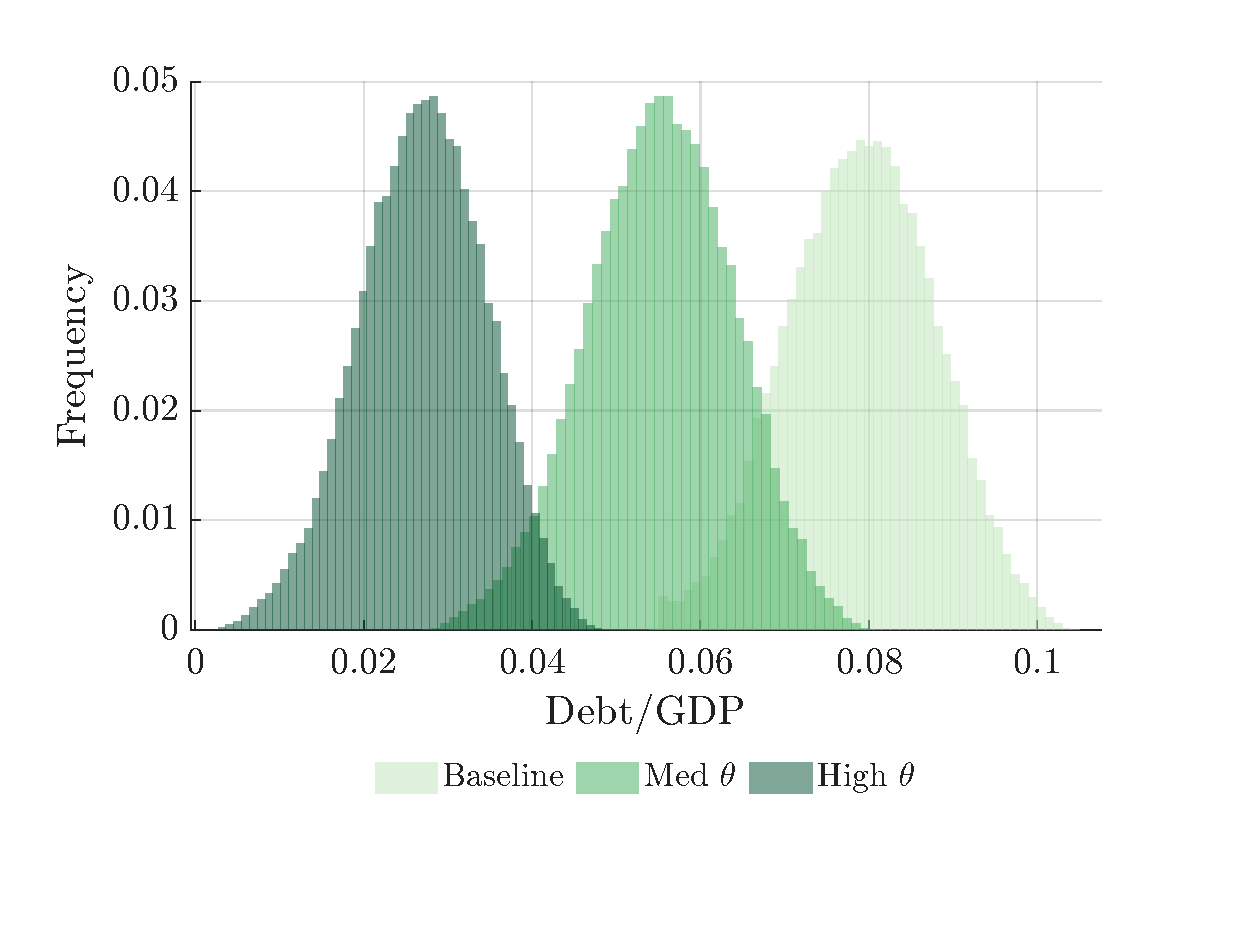
\includegraphics[width=\textwidth]{../../pro-default-model/results/comparison_figure_7.pdf}
		\caption{Debt-to-GDP Ratio Distribution}
		\label{fig:dist_debt}
	\end{subfigure}
	\hfill
	\begin{subfigure}[b]{0.48\textwidth}
		\centering
		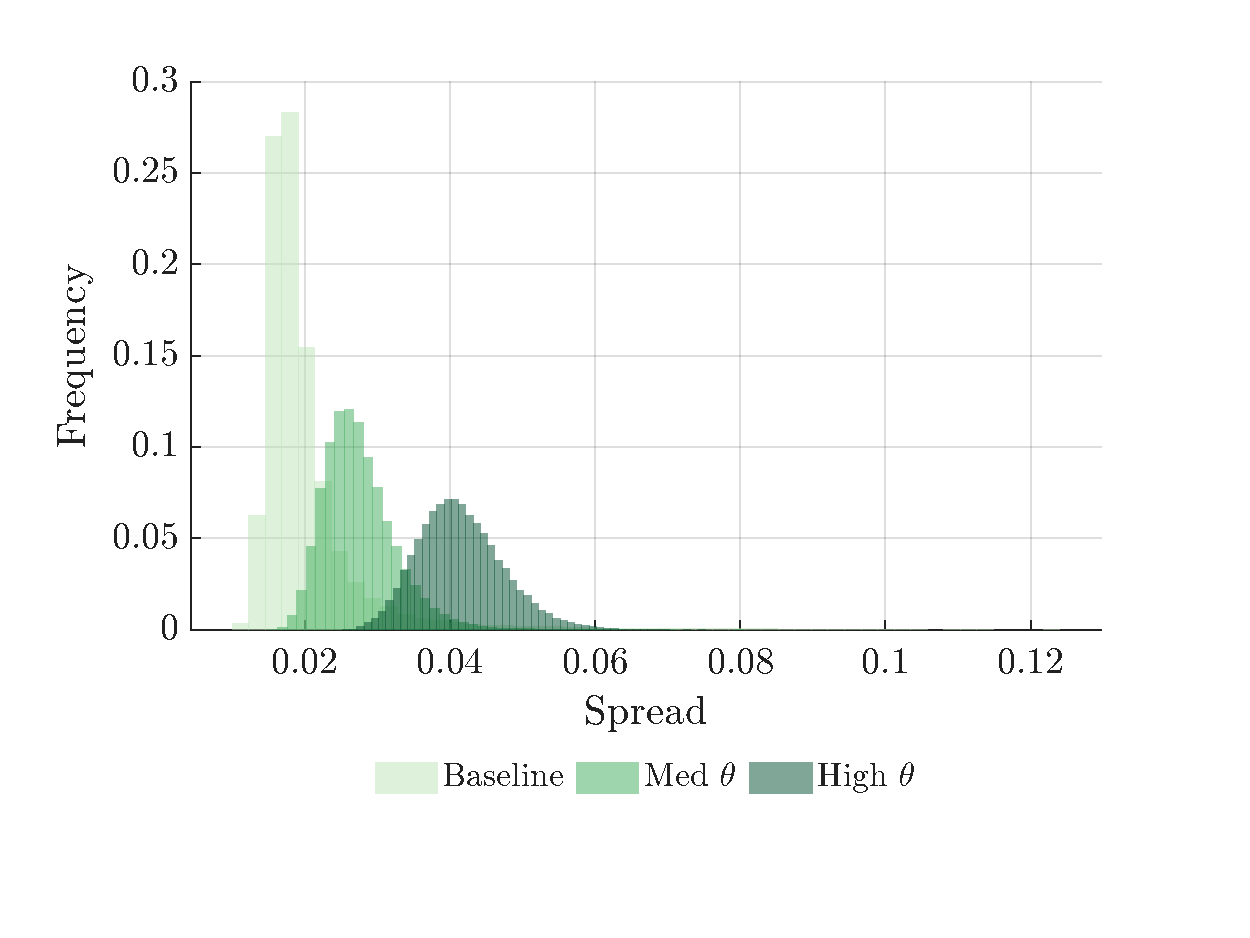
\includegraphics[width=\textwidth]{../../pro-default-model/results/comparison_figure_6.pdf}
		\caption{Credit Spread Distribution}
		\label{fig:dist_spread}
	\end{subfigure}
	\caption{Simulated Stationary Distributions}
	\label{fig:sim_distributions}
	\parbox{\linewidth}{\small\textit{Note:} The distributions are generated from a long simulation of the model (100,000 periods). The figure shows how rising PRO progressively shifts the long-run distribution of the debt-to-GDP ratio to the left (deleveraging) and the credit spread distribution to the right (higher borrowing costs).}
\end{figure}

\paragraph{State-Contingent Policies: The Pivoting Effect}
The long-run distributional shifts are driven by state-by-state changes in the
sovereign's optimal policies, which are themselves a reaction to the altered
price schedule. Figure~\ref{fig:policy_pivot} visualizes how PRO causes key
functions to "pivot" around the rational benchmark, providing a graphical
confirmation of the paper's central theoretical results.

Panels~\ref{fig:pivot_price} and~\ref{fig:pivot_spread} illustrate the core
price pivot. At low debt levels, where a rational lender sees little risk, the
PRO lender prices in the possibility of an "out of the blue" default, leading
to lower prices and higher spreads. At very high debt levels, where a rational
lender sees default as nearly certain, the PRO lender's belief in randomness
allows for a small chance of an "irrational" repayment, leading to
paradoxically better terms (the "softening of doom" effect). This pivot in the
price schedule is the key external force acting on the sovereign, and it offers
a richer dynamic than the simple downward price shift one might associate with
reputational deterioration under standard assumptions.

Panels~\ref{fig:pivot_default} and~\ref{fig:pivot_borrowing} show the
sovereign's endogenous response. The government internalizes the new price
schedule. The better terms available in the high-debt region increase the value

of maintaining market access, making the sovereign more resilient and pushing
out its default threshold (Proposition~\ref{prop:threshold}). More importantly,
in the normal course of borrowing, the sovereign faces worse prices, which act
as a higher effective cost of capital. The optimal response, shown in Panel
\ref{fig:pivot_borrowing}, is to deleverage and choose a lower next-period debt
level for any given state (Proposition~\ref{prop:deleveraging}).

\begin{figure}[h!]
	\centering
	\begin{subfigure}[b]{0.48\textwidth}
		\centering
		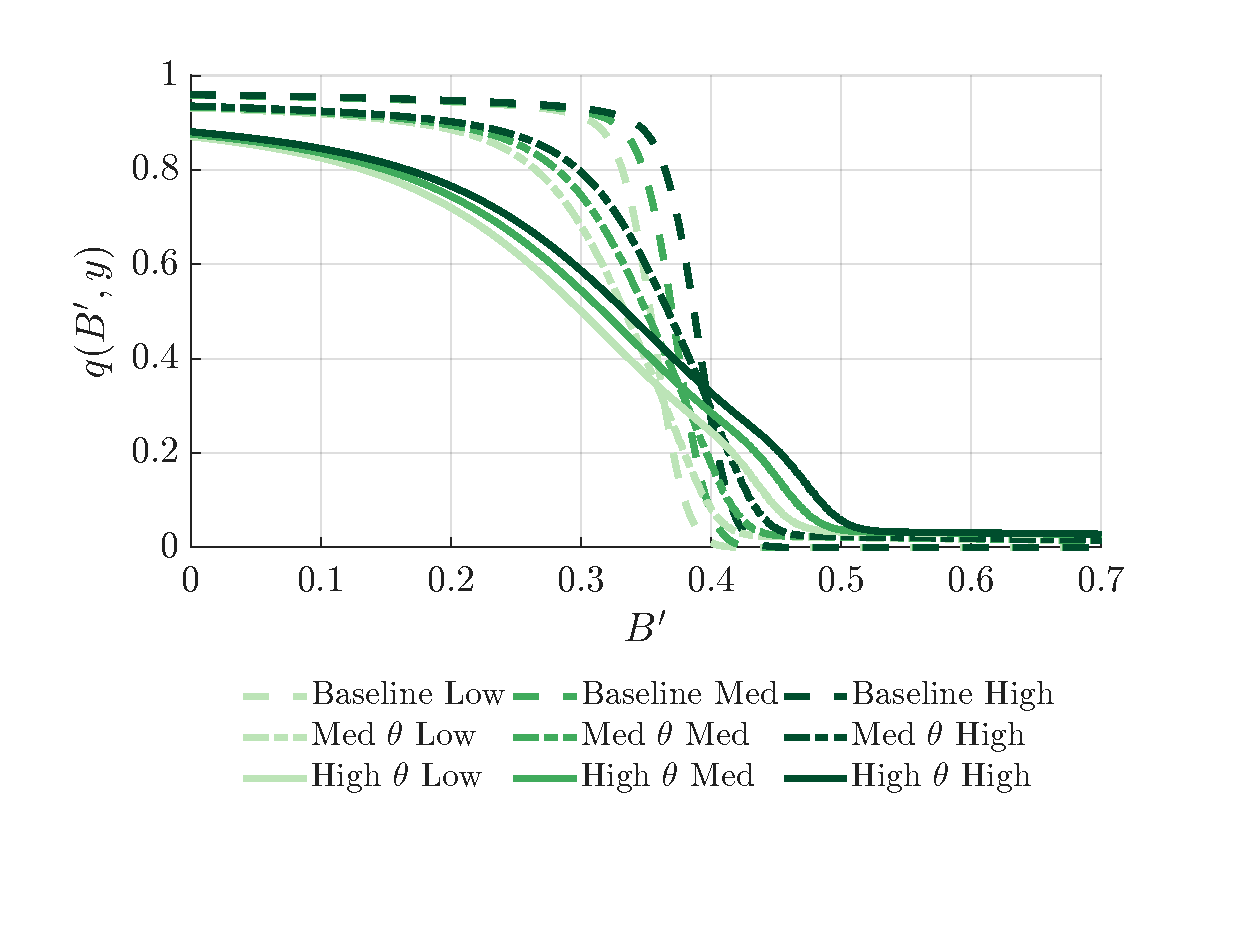
\includegraphics[width=\textwidth]{../../pro-default-model/results/comparison_figure_3.pdf}
		\caption{Bond Price Schedule, $q(B',y)$}
		\label{fig:pivot_price}
	\end{subfigure}
	\hfill
	\begin{subfigure}[b]{0.48\textwidth}
		\centering
		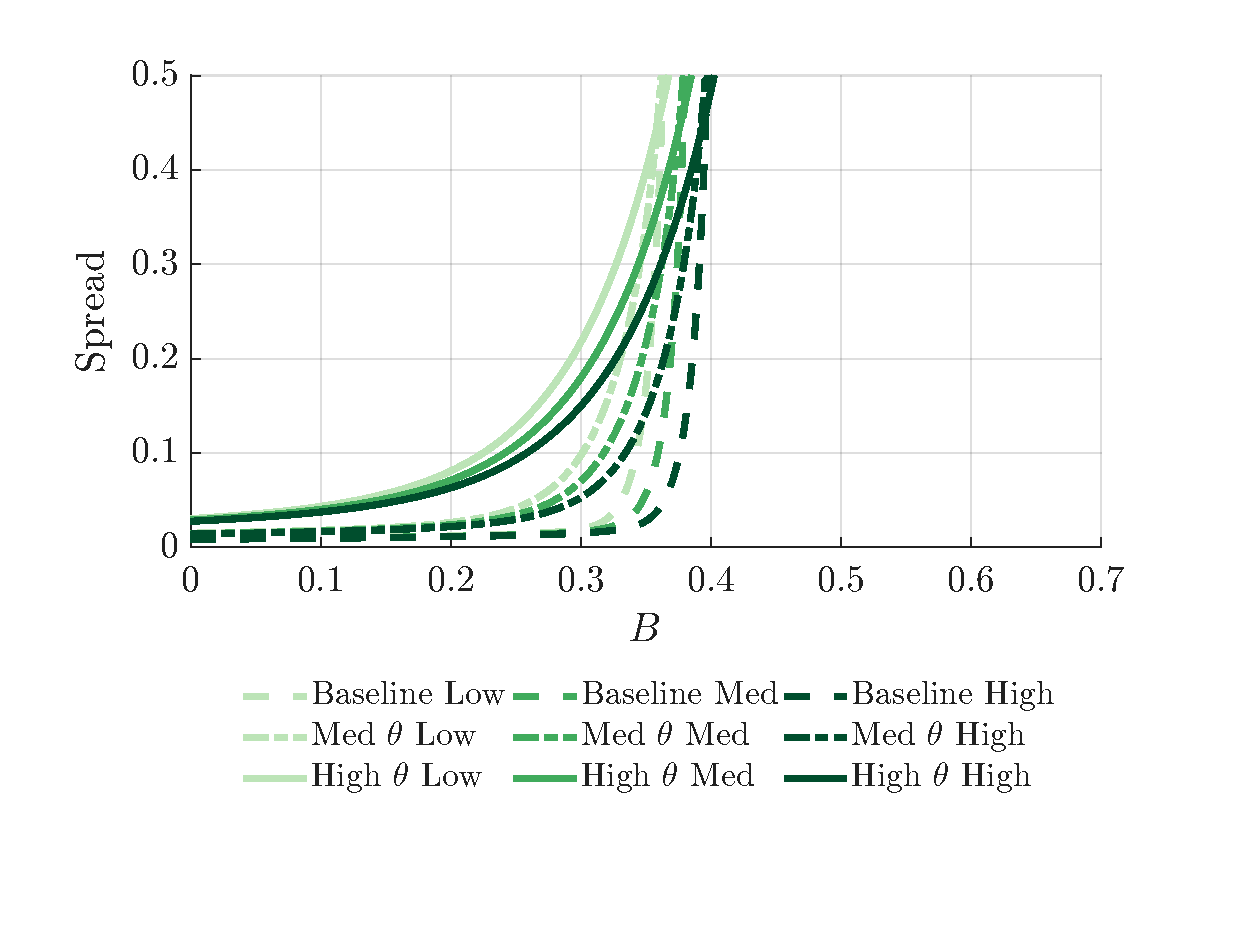
\includegraphics[width=\textwidth]{../../pro-default-model/results/comparison_figure_4.pdf}
		\caption{Credit Spread, $s(B',y)$}
		\label{fig:pivot_spread}
	\end{subfigure}
	\vskip\baselineskip
	\begin{subfigure}[b]{0.48\textwidth}
		\centering
		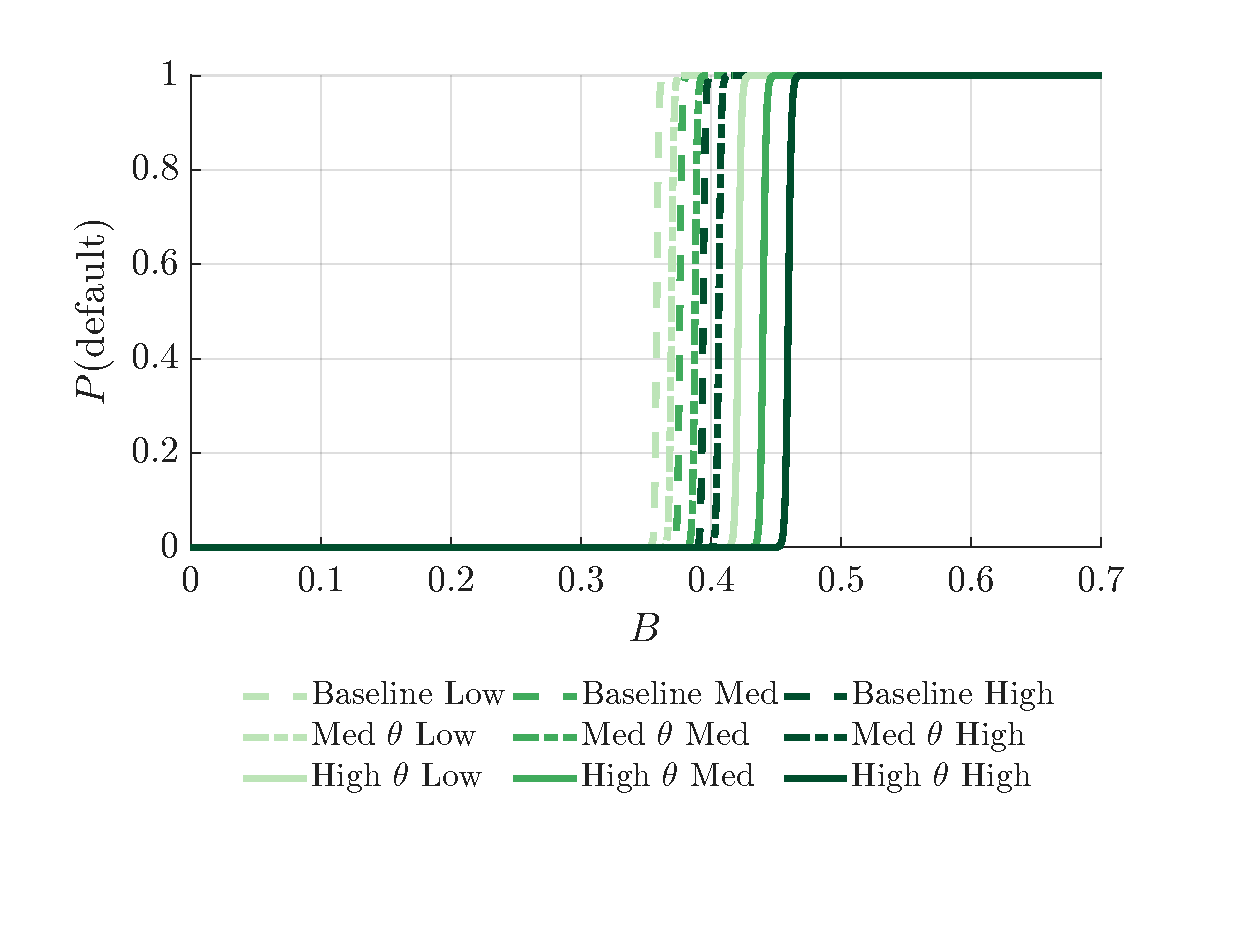
\includegraphics[width=\textwidth]{../../pro-default-model/results/comparison_figure_2.pdf}
		\caption{Default Probability, $P(d=1|B,y)$}
		\label{fig:pivot_default}
	\end{subfigure}
	\hfill
	\begin{subfigure}[b]{0.48\textwidth}
		\centering
		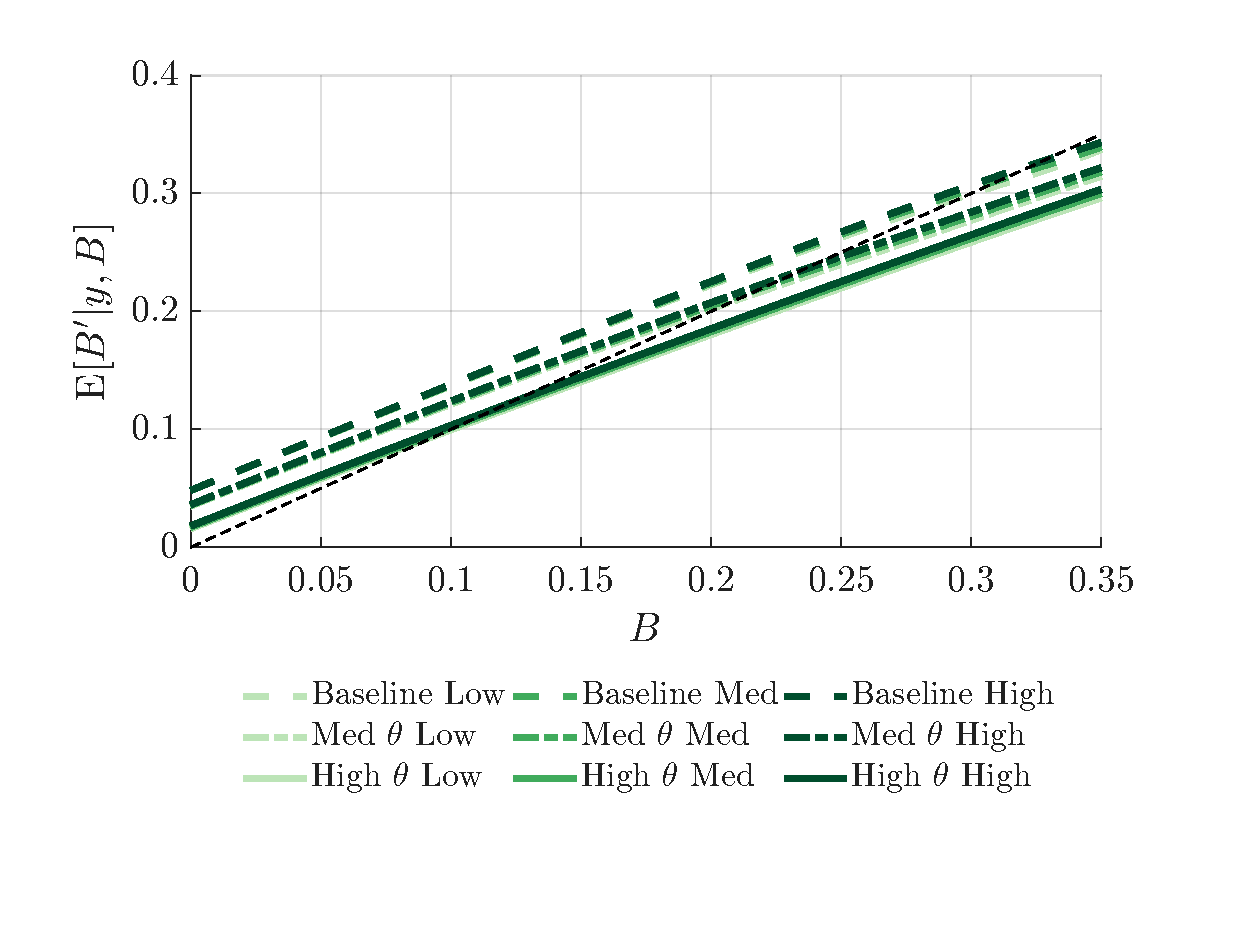
\includegraphics[width=\textwidth]{../../pro-default-model/results/comparison_figure_9.pdf}
		\caption{Borrowing Policy, $\mathbb{E}[B'|B,y]$}
		\label{fig:pivot_borrowing}
	\end{subfigure}
	\caption{Policy Function Pivoting}
	\label{fig:policy_pivot}
	\parbox{\linewidth}{\small\textit{Note:} The plots show the key policy and pricing functions for three different levels of endowment y (low, medium, and high). The functions for the baseline ($\theta=1$, dashed), medium PRO ($\theta=10$, dash-dot), and high PRO ($\theta=100$, solid) cases are shown. Rising PRO causes the functions to pivot.}
\end{figure}

\paragraph{Welfare Consequences}
The sovereign's policy adjustments—deleveraging and tolerating higher debt
before default—are optimal given the market it faces, but they cannot overcome
the fundamental handicap of dealing with paranoid lenders. Proposition
\ref{prop:welfare} predicted a direct welfare loss, a result powerfully
confirmed by Figure~\ref{fig:welfare_loss}. The sovereign's value function is
uniformly and significantly lower under higher PRO.

This welfare loss stems from the impairment of the sovereign's ability to
smooth consumption. Access to international credit markets is a tool to buffer
domestic shocks. PRO effectively places a tax on the use of this tool. By
making borrowing more expensive in the relevant range, it forces the sovereign
to either endure more volatile consumption or to self-insure by maintaining an
inefficiently low level of debt. The ``benefit'' of better prices in the
far-off, high-risk region is an option that is too remote and uncertain to
compensate for the persistent, day-to-day welfare losses incurred from being
forced to transact with a market that systematically overestimates its
propensity to fail.

\begin{figure}[h!]
	\centering
	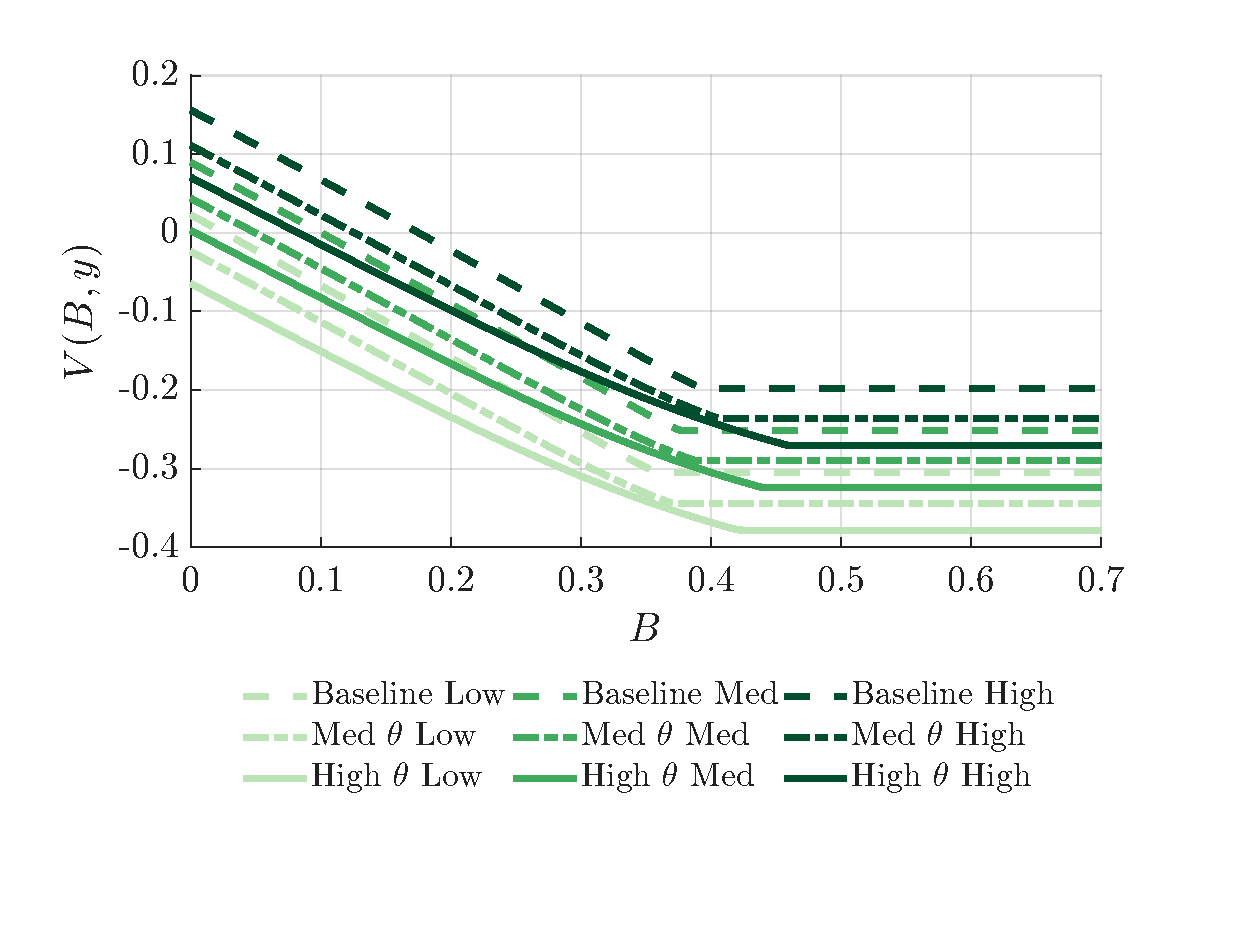
\includegraphics[width=0.6\textwidth]{../../pro-default-model/results/comparison_figure_1.pdf}
	\caption{Welfare Loss}
	\label{fig:welfare_loss}
	\parbox{\linewidth}{\small\textit{Note:} The figure plots the sovereign's ex-ante value function $V(y, B)$ for the baseline ($\theta=1$, dashed), medium PRO ($\theta=10$, dash-dot), and high PRO ($\theta=100$, solid) economies. The value function is uniformly lower under higher degrees of PRO, indicating a progressive welfare loss.}
\end{figure}

\subsection{Dynamic Responses and Adjustment Paths}

The dynamic implications of PRO reveal how PRO affects the sovereign's
adjustment paths and responses to shocks.

\paragraph{Deleveraging Dynamics: The Transition to Lower Debt}

Figure~\ref{fig:deleveraging_paths} traces optimal debt adjustment paths under
different initial conditions and degrees of PRO. Consistent with
Proposition~\ref{prop:deleveraging}, economies with higher PRO systematically
converge to lower debt levels regardless of starting point. Remarkably, even
from low initial debt, the high‑PRO economy continues deleveraging,
representing a fundamental fiscal shift rather than temporary adjustment.

The consumption and spread dynamics reveal important adjustment costs.
Panel~\ref{fig:consumption_path} shows that high‑PRO economies experience more
volatile consumption during deleveraging despite ultimately achieving lower
debt. Panel~\ref{fig:spread_path_delev} demonstrates that spreads remain
persistently elevated throughout adjustment, confirming that the ``PRO
premium'' reflects systematic risk overestimation at all debt levels rather
than just current leverage.

\begin{figure}[h]
	\centering
	\begin{subfigure}[b]{0.48\textwidth}
		\centering
		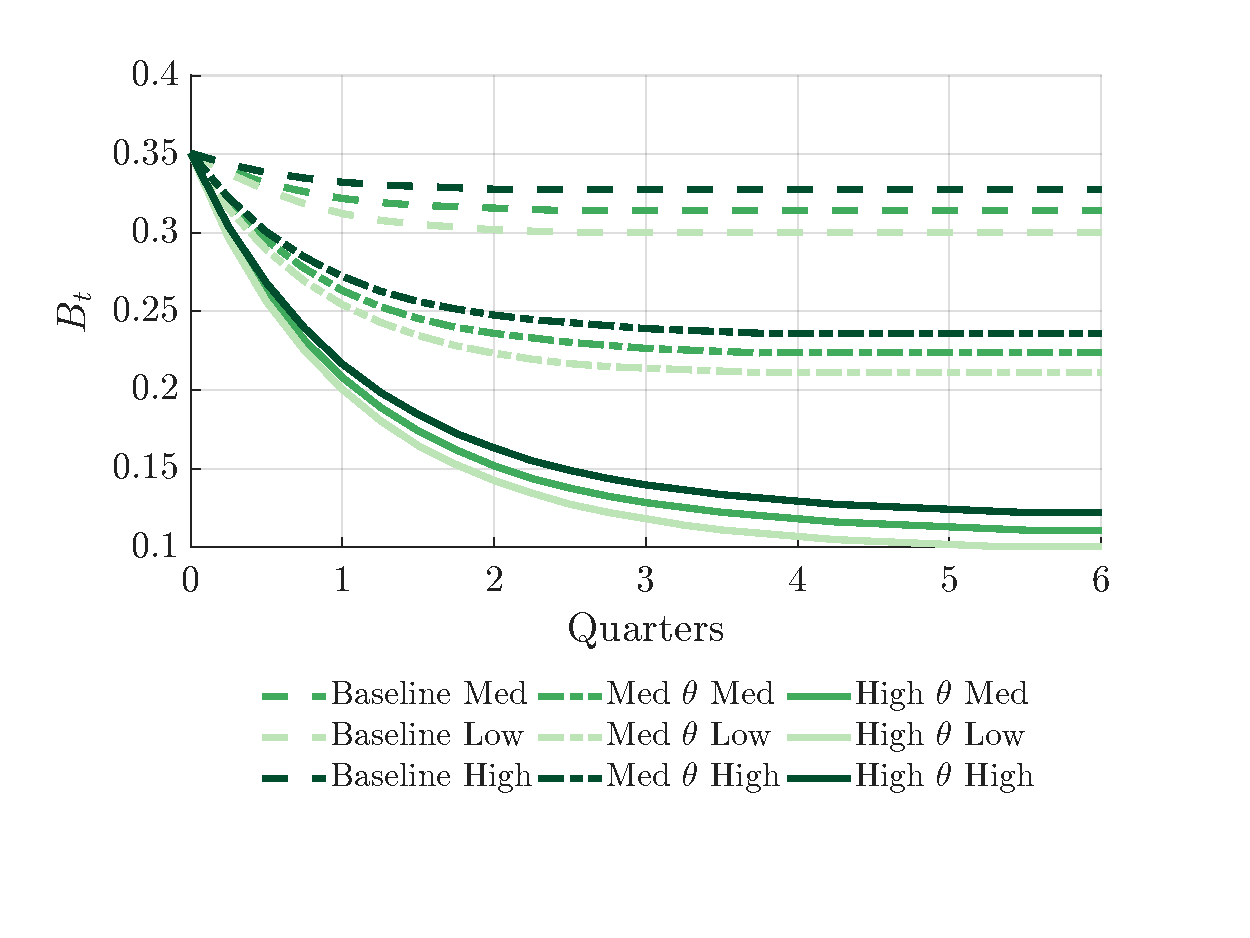
\includegraphics[width=\textwidth]{../../pro-default-model/results/comparison_figure_11.pdf}
		\caption{Debt}
		\label{fig:debt_path}
	\end{subfigure}
	\hfill
	\begin{subfigure}[b]{0.48\textwidth}
		\centering
		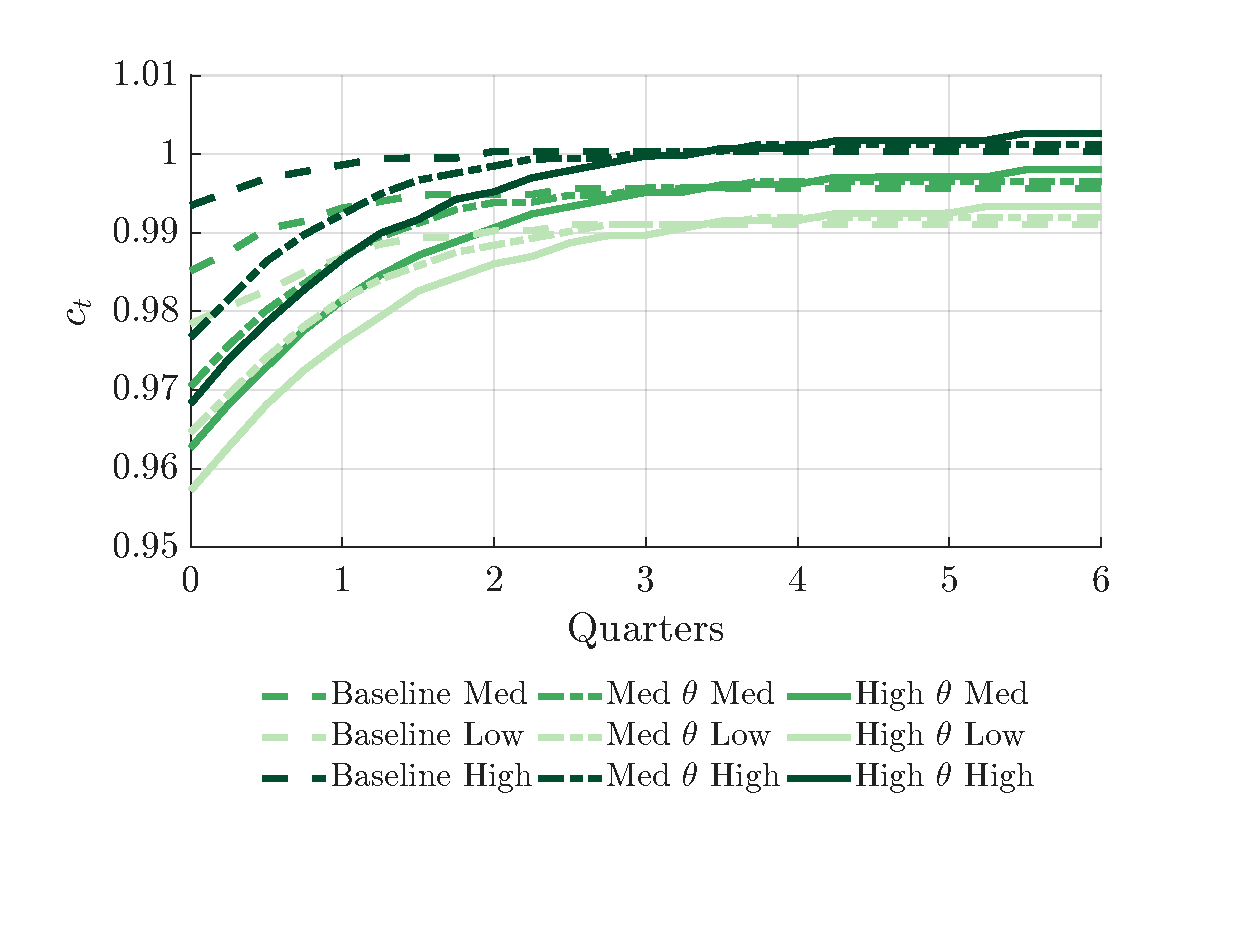
\includegraphics[width=\textwidth]{../../pro-default-model/results/comparison_figure_12.pdf}
		\caption{Consumption}
		\label{fig:consumption_path}
	\end{subfigure}
	\vskip\baselineskip
	\begin{subfigure}[b]{0.48\textwidth}
		\centering
		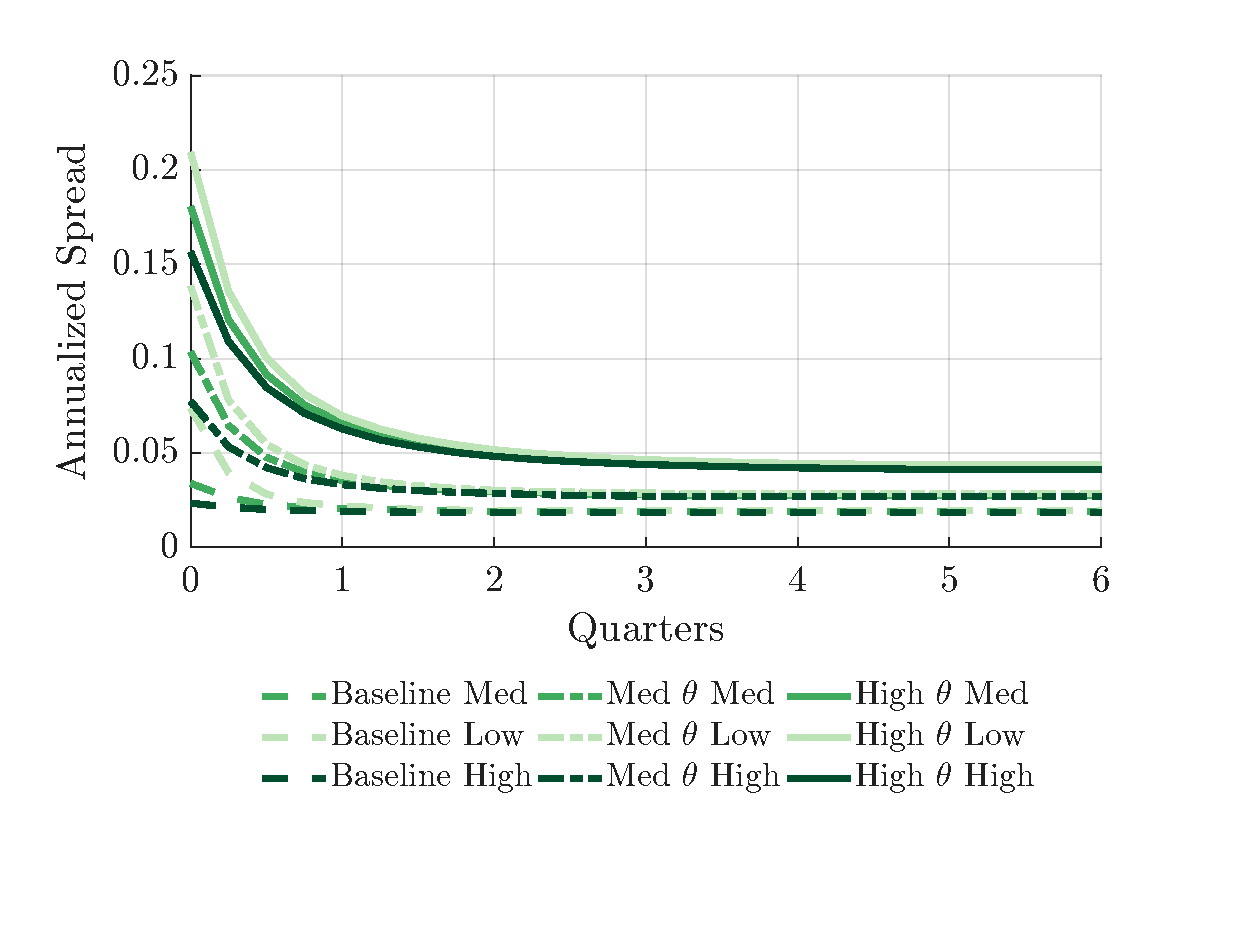
\includegraphics[width=\textwidth]{../../pro-default-model/results/comparison_figure_21.pdf}
		\caption{Spread}
		\label{fig:spread_path_delev}
	\end{subfigure}
	\caption{Deleveraging Dynamics}
	\label{fig:deleveraging_paths}
	\parbox{\linewidth}{\small\textit{Note:} The figure shows optimal adjustment paths over 6 quarters starting from three different initial debt levels (low, medium, high) for each degree of PRO. The paths demonstrate how PRO leads to systematic deleveraging that persists regardless of initial conditions, accompanied by persistently higher spreads and more volatile consumption during the transition.}
\end{figure}

\paragraph{Impulse Response Functions: Shock Propagation under PRO}

I examine responses to transitory and persistent productivity shocks (AR(1)
with $\rho = 0.8$) to understand how PRO affects the sovereign's shock
absorption capacity.

\subparagraph{Transitory Shock Responses.} Figure~\ref{fig:irf_transitory} shows responses to a 3\% positive productivity
shock lasting one quarter. While output effects are identical by construction
(panel~\ref{fig:irf_trans_output}), PRO fundamentally alters other responses.
High‑PRO economies exhibit muted debt reduction
(panel~\ref{fig:irf_trans_debt}) and consumption smoothing responses
(panel~\ref{fig:irf_trans_consumption}), illustrating impaired ability to
exploit temporary favorable conditions. Despite facing identical shocks, these
economies cannot fully capitalize on good fortune due to persistently
unfavorable credit pricing. Spreads fall in all economies
(panel~\ref{fig:irf_trans_spread}), but high‑PRO economies maintain higher
levels throughout adjustment.

\begin{figure}[h]
	\centering
	\begin{subfigure}[b]{0.48\textwidth}
		\centering
		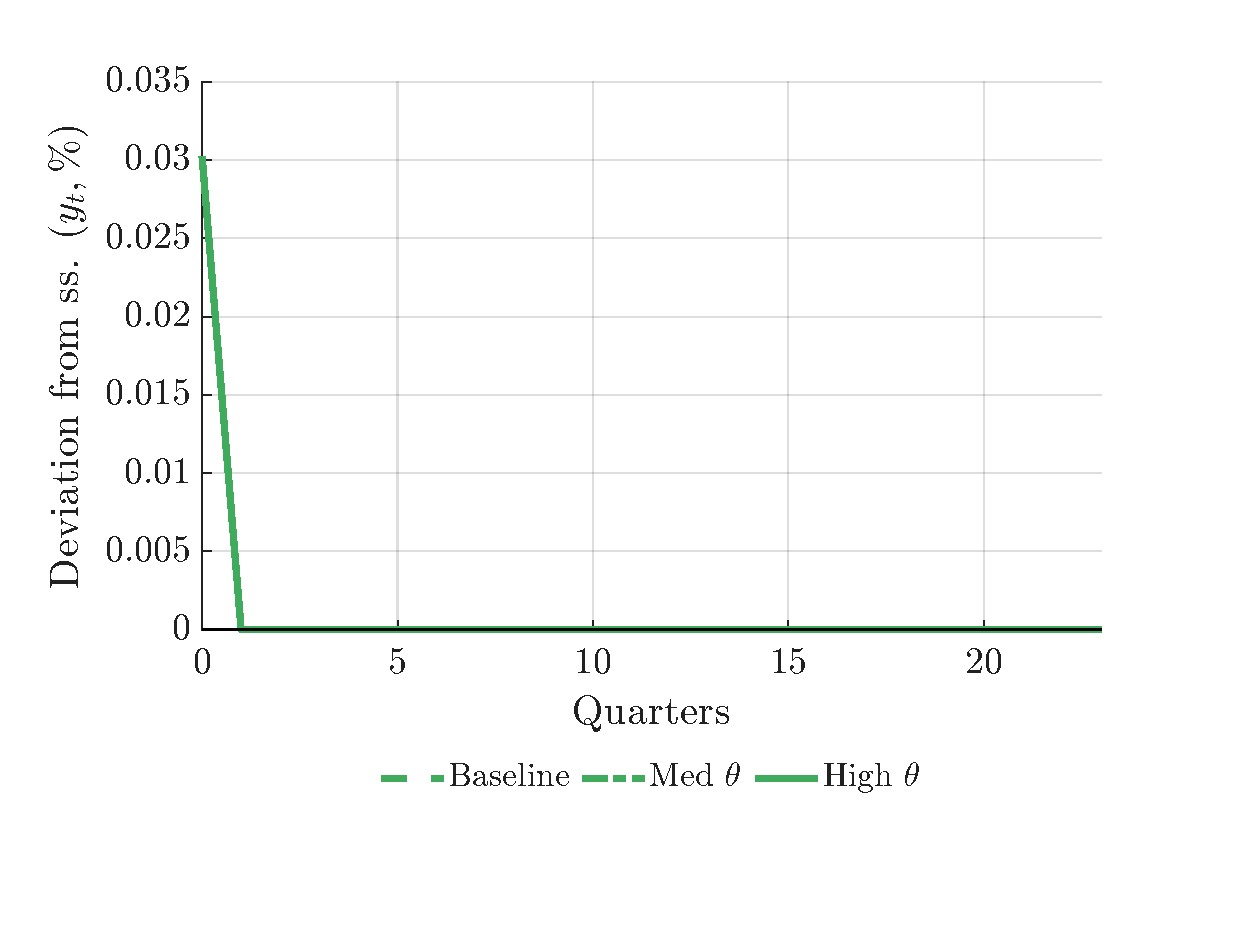
\includegraphics[width=\textwidth]{../../pro-default-model/results/comparison_figure_13.pdf}
		\caption{Output}
		\label{fig:irf_trans_output}
	\end{subfigure}
	\hfill
	\begin{subfigure}[b]{0.48\textwidth}
		\centering
		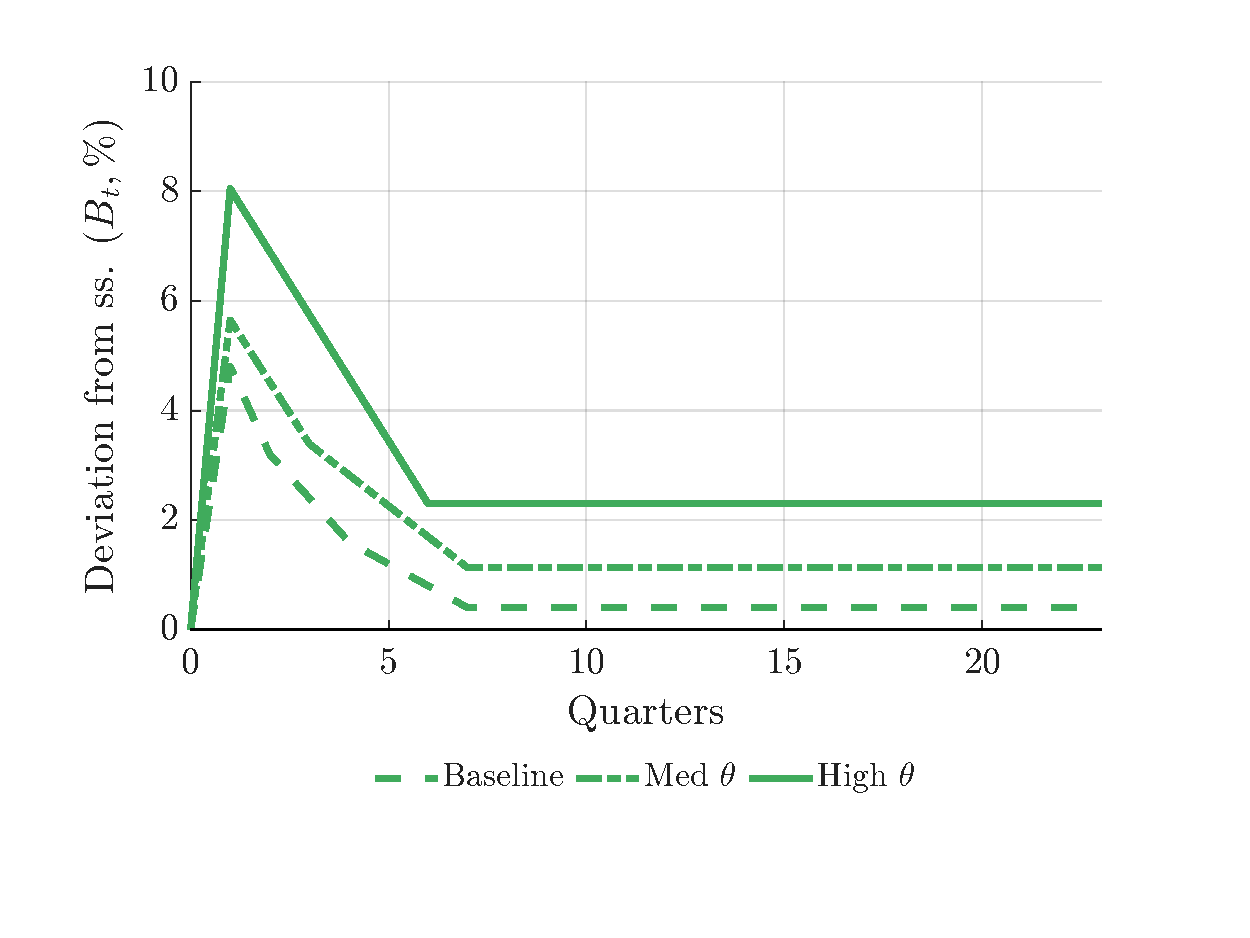
\includegraphics[width=\textwidth]{../../pro-default-model/results/comparison_figure_14.pdf}
		\caption{Debt}
		\label{fig:irf_trans_debt}
	\end{subfigure}
	\vskip\baselineskip
	\begin{subfigure}[b]{0.48\textwidth}
		\centering
		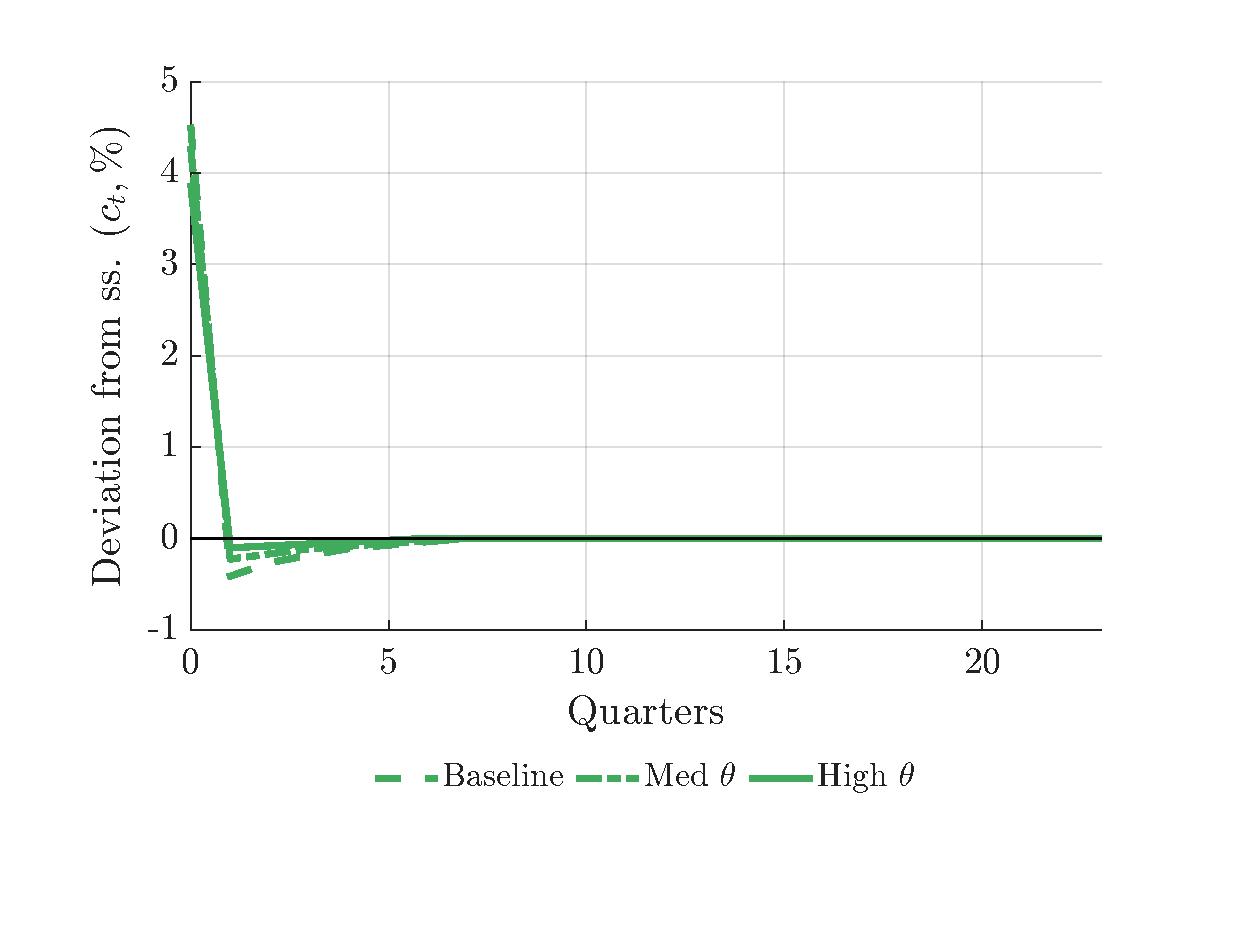
\includegraphics[width=\textwidth]{../../pro-default-model/results/comparison_figure_15.pdf}
		\caption{Consumption}
		\label{fig:irf_trans_consumption}
	\end{subfigure}
	\hfill
	\begin{subfigure}[b]{0.48\textwidth}
		\centering
		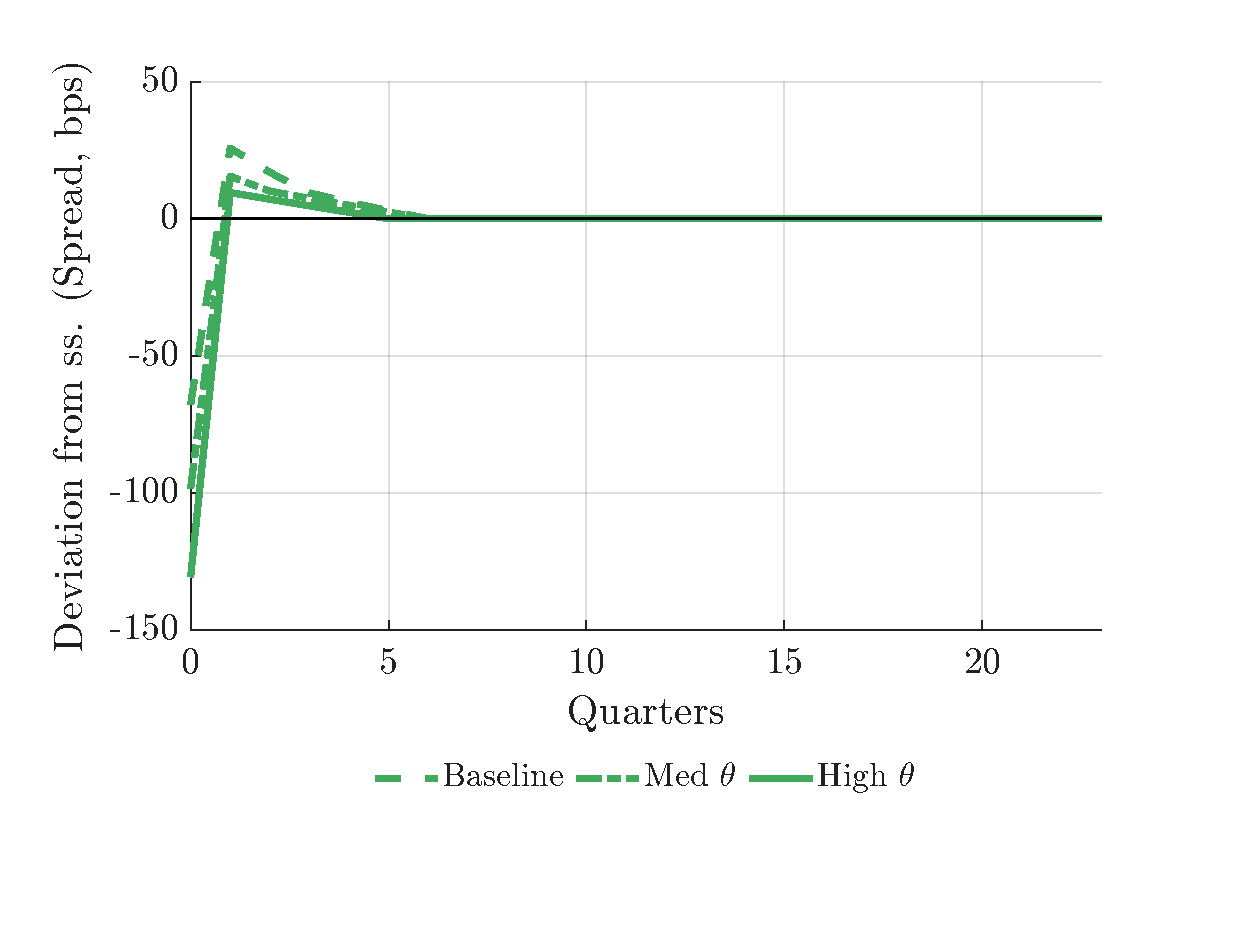
\includegraphics[width=\textwidth]{../../pro-default-model/results/comparison_figure_16.pdf}
		\caption{Spread}
		\label{fig:irf_trans_spread}
	\end{subfigure}
	\caption{Impulse Responses to Transitory Productivity Shock}
	\label{fig:irf_transitory}
	\parbox{\linewidth}{\small\textit{Note:} The figure shows responses to a 3\% positive productivity shock that lasts for one quarter. All variables are expressed as percentage deviations from their respective steady states (spreads in basis points). The responses demonstrate how PRO constrains the sovereign's ability to take advantage of temporary favorable conditions.}
\end{figure}

\subparagraph{Persistent Shock Responses.} Figure~\ref{fig:irf_persistent} shows responses to persistent productivity
shocks ($\rho = 0.8$). Persistence matters more for high-PRO economies, which
exhibit more pronounced and sustained debt reduction
(panel~\ref{fig:irf_pers_debt}) as sovereigns recognize rare opportunities to
escape the ``high-spread trap.'' While persistent shocks enable better
consumption smoothing across all economies
(panel~\ref{fig:irf_pers_consumption}), high-PRO economies still underperform
due to fundamental impairment of consumption insurance. Spread responses
(panel~\ref{fig:irf_pers_spread}) are more persistent than in the transitory
case, but high-PRO economies maintain higher levels throughout adjustment.

\begin{figure}[h]
	\centering
	\begin{subfigure}[b]{0.48\textwidth}
		\centering
		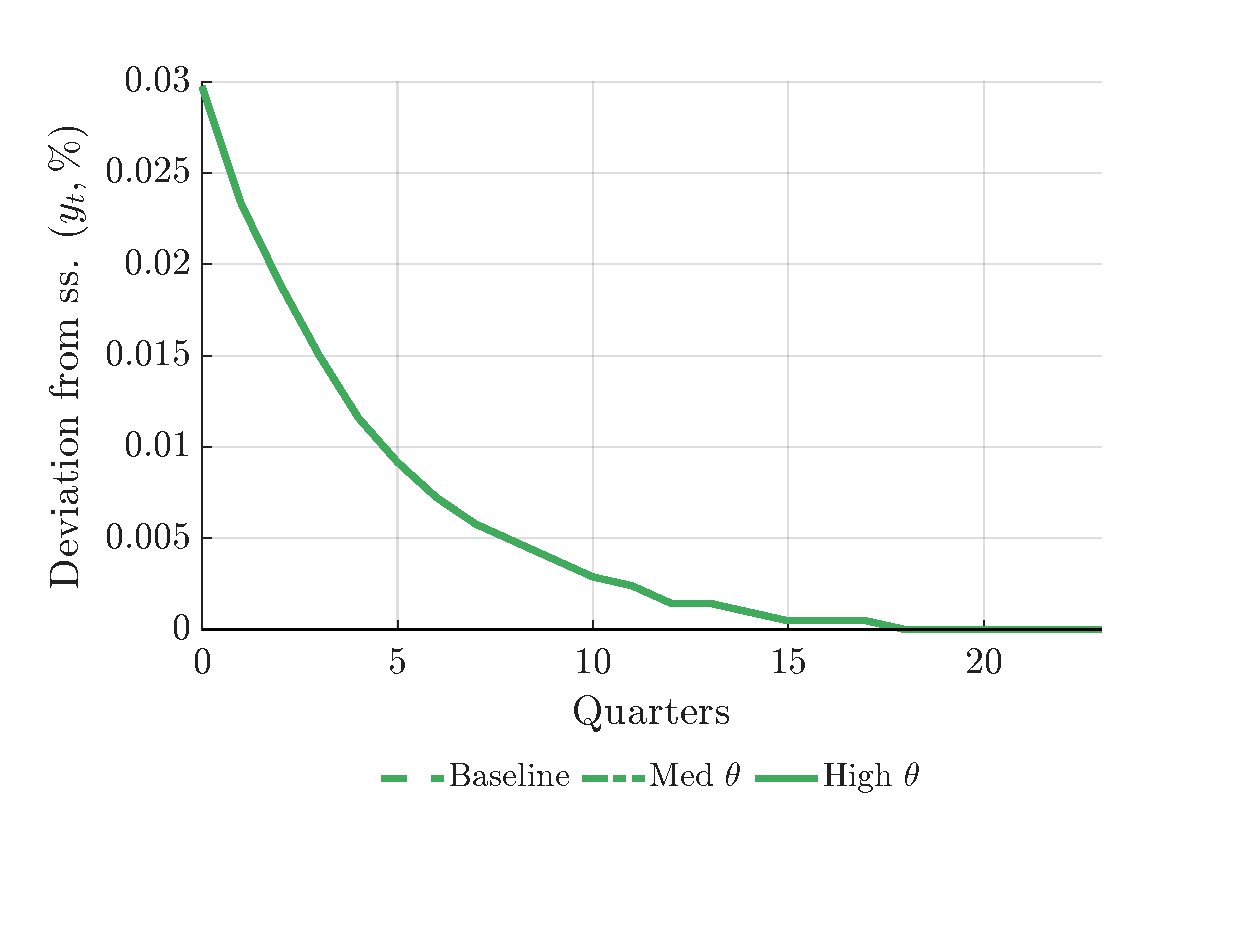
\includegraphics[width=\textwidth]{../../pro-default-model/results/comparison_figure_17.pdf}
		\caption{Output}
		\label{fig:irf_pers_output}
	\end{subfigure}
	\hfill
	\begin{subfigure}[b]{0.48\textwidth}
		\centering
		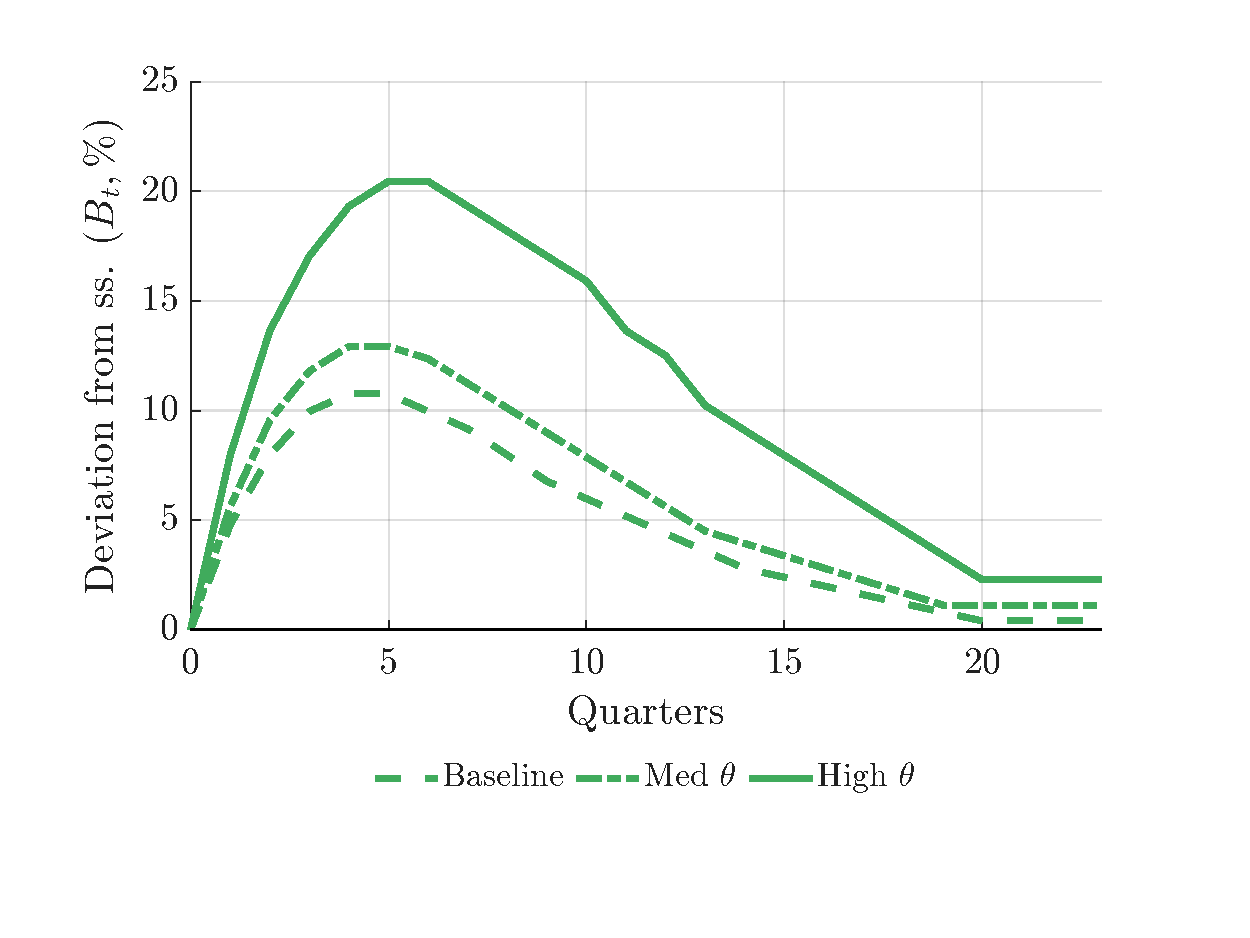
\includegraphics[width=\textwidth]{../../pro-default-model/results/comparison_figure_18.pdf}
		\caption{Debt}
		\label{fig:irf_pers_debt}
	\end{subfigure}
	\vskip\baselineskip
	\begin{subfigure}[b]{0.48\textwidth}
		\centering
		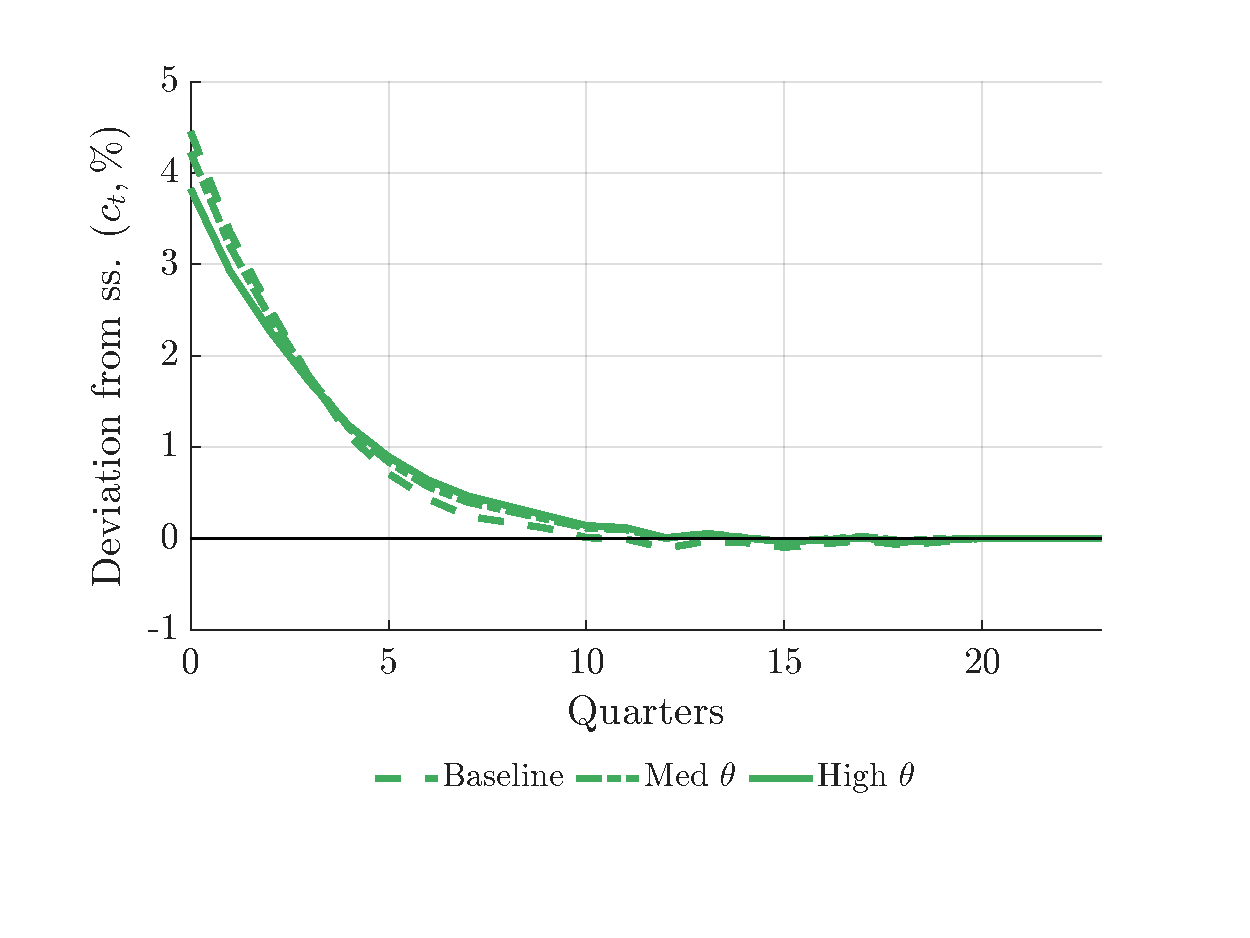
\includegraphics[width=\textwidth]{../../pro-default-model/results/comparison_figure_19.pdf}
		\caption{Consumption}
		\label{fig:irf_pers_consumption}
	\end{subfigure}
	\hfill
	\begin{subfigure}[b]{0.48\textwidth}
		\centering
		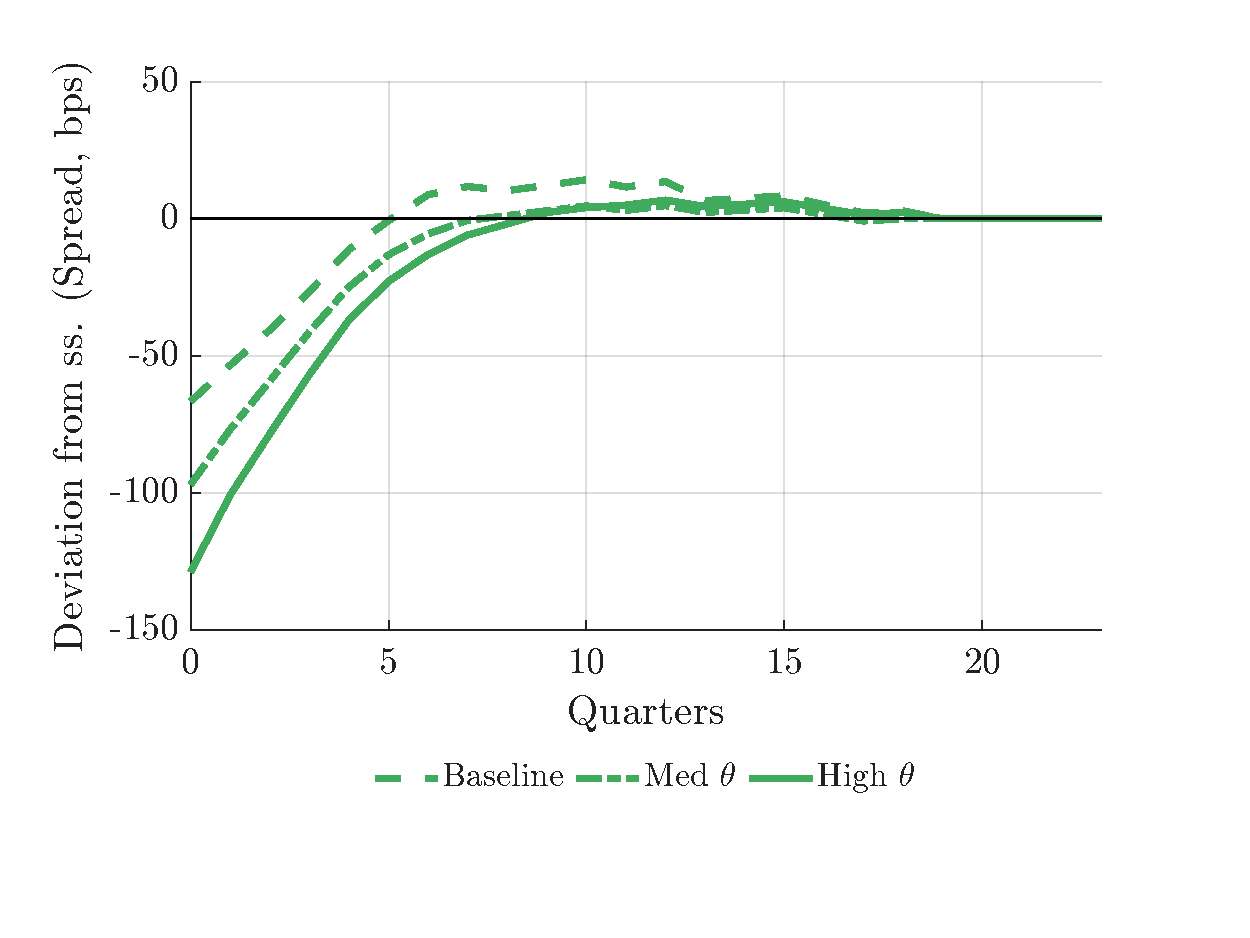
\includegraphics[width=\textwidth]{../../pro-default-model/results/comparison_figure_20.pdf}
		\caption{Spread}
		\label{fig:irf_pers_spread}
	\end{subfigure}
	\caption{Impulse Responses to Persistent Productivity Shock}
	\label{fig:irf_persistent}
	\parbox{\linewidth}{\small\textit{Note:} The figure shows responses to a 3\% productivity shock with autocorrelation $\rho = 0.8$. All variables are expressed as percentage deviations from steady state (spreads in basis points). The persistent nature of the shock reveals how PRO constrains fiscal flexibility even during extended periods of favorable fundamentals.}
\end{figure}

\paragraph{Implications}

The dynamic analysis reveals three fundamental economic mechanisms. First,
deleveraging under PRO creates persistent allocative distortions—the adjustment
process itself becomes a source of inefficiency as elevated spreads persist
throughout transition, generating deadweight losses that compound over time.
This represents a departure from standard models where adjustment costs are
temporary. Second, PRO creates asymmetric shock transmission: sovereigns
experience constrained benefits from favorable shocks while facing amplified
costs from adverse ones, fundamentally altering the risk-return profile of
sovereign borrowing. This asymmetry suggests that traditional moments-based
calibrations may understate welfare costs. Finally, the interaction between
persistence and beliefs generates hysteresis effects: temporary improvements in
fundamentals produce limited deleveraging, while sustained improvements are
necessary to overcome entrenched priors exhibiting PRO.

\section{Policy and Information Extensions}\label{sec:extensions}

\subsection{Theoretical Extensions}
This section remains within the same operator framework: I vary information and
policy mappings that enter \emph{through} the pricing operator $\mathcal
	T_\theta$, while holding primitives and the sovereign's choice aggregator
$J_\rho$ fixed.

\paragraph{Ramsey Planning Under PRO}\label{sec:ramsey}
Proposition~\ref{prop:welfare} shows that PRO reduces equilibrium welfare. A
natural question is whether an optimal fiscal authority can undo this loss. I
study a Ramsey planner who can choose lump-sum taxes/transfers but takes the
bond pricing mechanism as given. Formally, the planner's problem preserves the
same choice aggregator $J_\rho$, while bond prices are the unique fixed points
of the same operator $\mathcal T_\theta$; the planner's instruments enter only
the resource constraint and do not alter the pricing mechanism.

PRO acts like a persistent wedge in the intertemporal price of borrowing.
Transfers can reallocate resources within and across periods subject to a zero
present-value constraint, but they cannot change the shadow price at which the
government trades across dates. Hence the PRO price schedule distorts debt
choices even under optimal fiscal policy.

The planner chooses $\{c_t,B_{t+1},\tau_t\}_{t\ge0}$ to maximize expected
utility subject to the per-period resource constraint and a zero present-value
(PV) condition for transfers:
\begin{equation}
	c_t+\kappa B_t+\tau_t \;=\; y_t+\bigl(B_{t+1}-(1-\delta)B_t\bigr)\,q_\theta(y_t,B_{t+1}),
	\qquad t\ge0, \text{ a.s.}
	\label{eq:ramsey_rc}
\end{equation}
and
\begin{equation}
	\E_0\!\left[\sum_{t=0}^\infty \beta^t \tau_t\right]=0,
	\quad c_t\ge0,
	\quad B_{t+1}\in\mathcal B.
	\label{eq:ramsey_pv}
\end{equation}

\begin{proposition}
	\label{prop:ramsey_welfare}
	Let $r>-1$ satisfy $\beta(1+r)=1$. For $i\in\{1,\theta\}$ define the Ramsey value
	\[
		W^R_i \;=\; \sup_{\{c_t,B_{t+1},\tau_t\}}\E_0\!\Big[\sum_{t=0}^\infty \beta^t u(c_t)\Big]
	\]
	subject to~\eqref{eq:ramsey_rc}--\eqref{eq:ramsey_pv}. Assume:
	\begin{enumerate}
		\item[(A1)] $u$ is strictly increasing and strictly concave; $\mathcal B$ is compact.
		\item[(A2)] (Price dominance by trade sign, consistent with Propositions~\ref{prop:pivot_concise} and~\ref{prop:deleveraging}). Let $\Delta_t\equiv B_{t+1}-(1-\delta)B_t$. For every history,
		      \[
			      \Delta_t\ge0 \ \Rightarrow\ q_1(y_t,B_{t+1})\ge q_\theta(y_t,B_{t+1}),\qquad
			      \Delta_t\le0 \ \Rightarrow\ q_1(y_t,B_{t+1})\le q_\theta(y_t,B_{t+1}),
		      \]
		      with strict inequality on a set of positive probability and
		      $\Pr(|\Delta_t|>0)>0$.
	\end{enumerate}
	Then $W^R_\theta<W^R_1$.
\end{proposition}

\begin{proof}
	See Appendix~\ref{app:proof_ramsey}.
\end{proof}

Transfers ensure first-best \emph{conditional} consumption smoothing but cannot
change the intertemporal proceeds term $\E_0[\sum
	\beta^t\,\Delta_t\,q_i(y_t,B_{t+1})]$ that appears in the implementability
constraint; therefore the wedge in $q_\theta$ generates a genuine efficiency
loss. See also \citep{AiyagariMarcetSargentSeppala2002}.

\paragraph{Endogenous Belief Formation}
I next let lenders learn about the taste-shock dispersion parameter $\theta$.
This is a state augmentation of the baseline economy: I extend the state to
$S_t=(y_t,B_t,\theta_t)$ and keep the pricing operator unchanged except that it
is evaluated at the current belief, i.e., prices satisfy the same fixed-point
condition with $\mathcal T_{\theta_t}$.

Even with Bayesian updating, ``negativity bias''---overweighting unexpected
defaults relative to unexpected repayments---can make PRO persistent and
self-reinforcing. Rare but salient defaults move beliefs more than frequent,
modestly good realizations, creating a drift toward PRO.

Let $\theta_t\in[\underline\theta,\bar\theta]$ with
$\underline\theta=1<\bar\theta$, and suppose beliefs evolve according to
\begin{equation}
	\theta_{t+1}\;=\; \lambda\,\theta_t + (1-\lambda)\,\widehat\theta(\{d_s\}_{s=0}^t),
	\qquad \lambda\in(0,1),
	\label{eq:belief_updating}
\end{equation}
where $d_t\in\{0,1\}$ indicates default and $\widehat\theta(\cdot)$ is a (possibly biased) estimator that places extra weight on \emph{surprising} defaults. For instance, with
\begin{equation}
	\xi(y,B)\;=\;\max\!\left\{0,\ \frac{P_1(y,B)-P_{\theta_t}(y,B)}{P_1(y,B)}\right\},
	\label{eq:surprise_intensity}
\end{equation}
negativity bias means that $\widehat\theta$ responds more to larger $\xi$ when $d_t=1$ than to the analogous repayment surprise when $d_t=0$  \citep{BaumeisterBratslavskyFinkenauer2001,BordaloGennaioliShleifer2018}.

\begin{proposition}\label{prop:endogenous_beliefs}
	Under a stable, Feller belief-update kernel induced by~\eqref{eq:belief_updating} with negativity bias as above and mild drift/minorization conditions, the Markov process $\{\theta_t\}$ admits a unique invariant distribution $\Theta^*$ such that:
	\begin{enumerate}
		\item[\textbf{(i)}] $\E[\Theta^*]>1$ (persistent PRO);
		\item[\textbf{(ii)}] $\Theta^*$ first-order stochastically dominates the rational benchmark (history dependence through rare defaults);
		\item[\textbf{(iii)}] $\|\E[\theta_t]-\E[\Theta^*]\|=O(\lambda^t)$, with slow convergence when defaults are rare (large $\lambda$).
	\end{enumerate}
\end{proposition}

\begin{proof}
	See Appendix~\ref{app:proof_endogenous_beliefs}.
\end{proof}

\paragraph{Rational Inattention to Second Moments}
Still within the same operator framework, I microfound PRO as an optimal
attention allocation over first- versus second-moment information. Lenders
observe two signals about the sovereign's fundamentals: a mean signal $s_\mu$
and a dispersion (second-moment) signal $s_\sigma$. They choose precisions
$a_\mu,a_\sigma\ge0$ subject to a convex information cost, for instance
$\Phi(a_\mu,a_\sigma)=\tfrac{\kappa_\mu}{2}a_\mu^2+\tfrac{\kappa_\sigma}{2}a_\sigma^2$.
Higher $a_\sigma$ tightens beliefs about tail risk and thus lowers the
effective dispersion they attach to policy realizations.

Let $\theta$ summarize the dispersion/tail weight inside the same pricing
operator $\mathcal T_\theta$. Under rational inattention, $\theta$ becomes
endogenous: $\theta_{\mathrm{RI}}(y,B') =
	1+\varphi\,g\!\big(a_\sigma(y,B')\big)$ with $\varphi>0$ and $g$ increasing,
and prices still solve the \emph{same} fixed-point condition with $\mathcal
	T_{\theta_{\mathrm{RI}}(y,B')}$. The optimal attention vector solves
\[
	\max_{a_\mu,a_\sigma\ge0}\; \E\big[U\,|\,a_\mu,a_\sigma\big] - \Phi(a_\mu,a_\sigma),
\]
where the marginal value of $a_\sigma$ is proportional to how strongly prices
react to dispersion in the current state $(y,B')$. Because the price schedule
is steeper in states with higher default sensitivity, the FOC implies
state-dependent attention to dispersion:
\begin{equation}
	\frac{\partial a_\sigma(y,B')}{\partial \text{stress}}\;>\;0
	\quad\Rightarrow\quad
	\frac{\partial \theta_{\mathrm{RI}}(y,B')}{\partial \text{stress}}\;>\;0.
	\label{eq:ri_comparative_static}
\end{equation}

\begin{proposition}[Within-baseline comparative statics under RI]
	\label{prop:ri_maintains_results}
	Suppose $\Phi$ is strictly convex and separable and that attention raises the
	weight on dispersion monotonically as in~\eqref{eq:ri_comparative_static}.
	Then the operator $\mathcal T_{\theta_{\mathrm{RI}}(\cdot)}$ remains positive
	and order-preserving on prices. Consequently, the baseline results—single-
	crossing price pivot at $B^*(y)$, $B^*(y)$ increasing in $y$, and
	deleveraging alongside higher mean spreads—continue to hold as within-baseline
	comparative statics with $\theta$ replaced by $\theta_{\mathrm{RI}}(y,B')$.
\end{proposition}

\begin{proof}
	Positivity and order preservation are inherited from $\mathcal T_\theta$ pointwise
	in $(y,B')$; continuity of $\theta_{\mathrm{RI}}$ and the monotone mapping in
	\eqref{eq:ri_comparative_static} preserve the lattice and fixed-point
	arguments used in the baseline propositions.
\end{proof}

Empirically, exogenous reductions in the cost of dispersion-relevant
information (e.g., disclosure reforms or standardized risk reporting) should
compress spreads disproportionately in high-debt/high-stress states, flatten
the price pivot, and lower the default threshold—all testable within event
studies or difference-in-differences designs.

\paragraph{Optimal Policy Communication}
This extension likewise preserves the baseline structure: transparency affects
only the \emph{effective} belief input into the same pricing operator, while
the sovereign's choice aggregator $J_\rho$ and other primitives are unchanged.
Now allow the government to choose a transparency level $\alpha\in[0,1]$ that
affects lenders' effective dispersion:
\begin{equation}
	\theta_{\mathrm{eff}}(\alpha,\theta)\;=\;\alpha\cdot 1 + (1-\alpha)\cdot \theta,
	\label{eq:effective_theta}
\end{equation}
and let period utility be $u(c,\alpha)=c^{1-\sigma}/(1-\sigma)-\phi(\alpha)$ with $\phi(\alpha)=\gamma\alpha^2/2$.

\begin{proposition}\label{prop:optimal_communication}
	Let $W(\alpha)$ be the sovereign's value when the price schedule is $q_{\theta_{\mathrm{eff}}(\alpha,\theta)}$ and the planner otherwise solves the same Ramsey problem. Suppose $W(\alpha)$ is strictly concave in $\alpha$ (e.g., $q_\vartheta$ is smooth and $\phi$ is strictly convex). Then:
	\begin{enumerate}
		\item[\textbf{(i)}] There exists a unique $\alpha^*\in[0,1]$ satisfying the FOC
		      \begin{equation}
			      \frac{d}{d\alpha}W(\alpha^*) \;=\; \phi'(\alpha^*) \;=\; \gamma\,\alpha^*.
			      \label{eq:foc_transparency}
		      \end{equation}
		\item[\textbf{(ii)}] If $\partial W/\partial \vartheta<0$ and $\partial \theta_{\mathrm{eff}}/\partial \alpha=1-\theta<0$, then $\partial \alpha^*/\partial \theta>0$: greater PRO raises optimal transparency.
		\item[\textbf{(iii)}] There exists $\theta_c>1$ such that $W(\alpha^*)>W(0)$ for all $\theta>\theta_c$.
	\end{enumerate}
\end{proposition}

\begin{proof}
	See Appendix~\ref{app:proof_optimal_communication}.
\end{proof}

Transparency improves welfare by steepening lenders' price schedule toward the
rational benchmark, but convex disclosure costs imply an interior optimum. The
comparative static in (ii) formalizes that transparency is most valuable when
PRO is severe.

\paragraph{Testable Predictions and Empirical Hooks}
As brief guidance for future empirical work, the framework yields concise,
testable implications: (i) a single-crossing pivot in price/spread schedules
with $B^*(y)$ increasing in $y$; (ii) higher default thresholds despite higher
average spreads; (iii) deleveraging alongside higher mean spreads and lower
volatility (``stability illusion''); and (iv) cross-maturity and peer
``decoupling'' patterns consistent with second-moment (dispersion) beliefs. I
view these as light-touch empirical hooks—for calibration and event studies
(e.g., Argentina)—rather than the focus here.

\section{Conclusion}

Standard models struggle to explain why emerging economies face persistently
high borrowing costs. This paper develops a quantitative sovereign default
model with a behavioral friction---policy-randomness overestimation (PRO)---to
address this puzzle. I assume lenders systematically overestimate the
randomness of the sovereign's policy choices. Theoretically, this PRO wedge
does not uniformly depress bond prices but instead \textit{pivots} the price
schedule, making debt cheaper at the edge of default but more expensive in
normal times. A rational sovereign responds to these altered incentives in
counterintuitive ways: it tolerates a higher debt burden before defaulting, yet
simultaneously deleverages its day-to-day borrowing. Quantitatively, the model
shows that high PRO can force the debt-to-GDP ratio down from 7.90\% to 2.70\%,
while more than doubling the average credit spread from 2.00\% to 4.15\%. This
deleveraging creates an ``illusion of financial stability,'' where observable
market volatility falls even as financial cycles are amplified and the
sovereign's welfare declines.

I view PRO as complementary to reputation‑based learning rather than a
substitute. A joint empirical strategy that leverages maturity‑specific
responses to informational shocks, the shape of the price schedule, and the
evolution of volatility can help separate first‑moment (type) from
second‑moment (dispersion) channels. In practice, both mechanisms may operate
simultaneously.

The theoretical extensions provide additional insights. Even optimal Ramsey
fiscal policy cannot eliminate the welfare costs of PRO because the distorted
bond pricing creates fundamental allocative distortions that transfers cannot
correct. When beliefs are formed endogenously through Bayesian learning with
negativity bias, perceptions exhibiting PRO become self-reinforcing and persist
over time, explaining why some economies face chronically high borrowing costs.
However, governments can partially mitigate these effects through strategic
policy communication, choosing optimal transparency levels to reduce perceived
uncertainty while managing the costs of information disclosure. My work thus
offers a new, behaviorally-grounded perspective on sovereign risk,
demonstrating how market beliefs can be a fundamental driver of debt crises and
highlighting the importance of optimal policy design in managing these
behavioral frictions.

\clearpage
\appendix

% Reset equation counter and redefine equation numbering for appendices
\setcounter{equation}{0}
\renewcommand{\theequation}{\thesection.\arabic{equation}}

\begin{center}
	\Large \textbf{Appendices for ``Default with Policy-Randomness Overestimation''}\\
	\vspace{0.5cm}
	\large \textbf{Chen Gao}
	\\
	\large \today
\end{center}

This appendix contains the details of the Gumbel distribution and the proofs
for the lemmas and propositions in the paper. Section~\ref{app:gumbel} contains
the details of the Gumbel distribution. Section~\ref{app:proofs} contains the
proofs for the lemmas and propositions in the paper.
Section~\ref{app:computations} contains the computational algorithm details for
the model, including the numerical stability techniques employed in the
discrete choice implementation.

\section{Gumbel Distribution in Default Models}\label{app:gumbel}
In this section, I provide some useful results about the Gumbel distribution to
help formulate the close form solution presented in Section \ref{sec:model}.

\begin{lemma}
	\label{lem:gumbel_max_expectation}
	Let $\varepsilon_1, \varepsilon_2$ be independent random variables distributed as Gumbel$(-\eta\gamma, \eta)$, where $\gamma$ is the Euler-Mascheroni constant. Let $V_1, V_2 \in \mathbb{R}$ be deterministic constants. Then:
	\begin{equation}
		\mathbb{E}\left[\max\{V_1 + \varepsilon_1, V_2 + \varepsilon_2\}\right] = \eta \ln\left( \exp\frac{V_1}{\eta} + \exp\frac{V_2}{\eta} \right).
	\end{equation}
\end{lemma}

\begin{proof}
	See Appendix~\ref{app:proof_gumbel_max_expectation}.
\end{proof}

\begin{lemma}
	\label{lem:gumbel_logit}
	Let $\varepsilon_1, \varepsilon_2$ be independent Gumbel$(-\eta\gamma, \eta)$ random variables, and let $V_1, V_2 \in \mathbb{R}$ be deterministic values. Then:
	\begin{equation}
		\Pr\{V_1 + \varepsilon_1 > V_2 + \varepsilon_2\} = \frac{\exp\frac{V_1}{\eta}}{\exp\frac{V_1}{\eta} + \exp\frac{V_2}{\eta}}.
	\end{equation}
\end{lemma}

\begin{proof}
	See Appendix~\ref{app:proof_gumbel_logit}.
\end{proof}

\begin{lemma}
	\label{lem:gumbel_multinomial}
	Let $\{V_i\}_{i=1}^n$ be deterministic values and $\{\varepsilon_i\}_{i=1}^n$ be independent Gumbel$(-\sigma\gamma, \sigma)$ random variables. Then:
	\begin{align}
		\mathbb{E}\left[\max_{i \in \{1,\ldots,n\}} \{V_i + \varepsilon_i\}\right]    & = \sigma \ln\left( \sum_{i=1}^n \exp\frac{V_i}{\sigma} \right),       \\
		\Pr\left\{\arg\max_{i \in \{1,\ldots,n\}} \{V_i + \varepsilon_i\} = j\right\} & = \frac{\exp\frac{V_j}{\sigma}}{\sum_{i=1}^n \exp\frac{V_i}{\sigma}}.
	\end{align}
\end{lemma}

\begin{proof}
	See Appendix~\ref{app:proof_gumbel_multinomial}.
\end{proof}

\section{Proofs}\label{app:proofs}
This section contains the proofs for the lemmas and propositions in the paper.

\subsection{Proof of Lemma~\ref{lem:gumbel_max_expectation}}\label{app:proof_gumbel_max_expectation}

\begin{proof}
	Let $X_1 = V_1 + \varepsilon_1$ and $X_2 = V_2 + \varepsilon_2$, where $\varepsilon_1, \varepsilon_2$ are independent Gumbel$(-\eta\gamma, \eta)$ random variables. I derive the expected value $\mathbb{E}[\max\{X_1, X_2\}]$. The CDF of a Gumbel$(\mu, \sigma)$ random variable is $F(x; \mu, \sigma) =
		\exp(-\exp(-(x - \mu)/\sigma))$. For the parametrization Gumbel$(-\eta\gamma,
		\eta)$:
	\begin{equation*}
		F_\varepsilon(x) = \exp\left(-\exp\left(-\frac{x}{\eta} - \gamma\right)\right).
	\end{equation*}
	The CDF of $X_i = V_i + \varepsilon_i$ is obtained by translation:
	\begin{equation*}
		F_{X_i}(x) = F_\varepsilon(x - V_i) = \exp\left(-\exp\left(-\frac{x - V_i}{\eta} - \gamma\right)\right).
	\end{equation*}
	The CDF of $\max\{X_1, X_2\}$ is:
	\begin{align*}
		F_{\max}(x) & = \Pr\{\max\{X_1, X_2\} \leq x\} = \Pr\{X_1 \leq x, X_2 \leq x\}                                                                            \\
		            & = F_{X_1}(x) \cdot F_{X_2}(x)                                                                                                               \\
		            & = \exp\left(-\exp\left(-\frac{x - V_1}{\eta} - \gamma\right)\right) \cdot \exp\left(-\exp\left(-\frac{x - V_2}{\eta} - \gamma\right)\right) \\
		            & = \exp\left(-\exp\left(-\frac{x - V_1}{\eta} - \gamma\right) - \exp\left(-\frac{x - V_2}{\eta} - \gamma\right)\right)                       \\
		            & = \exp\left(-e^{-\gamma}\left(\exp\left(-\frac{x - V_1}{\eta}\right) + \exp\left(-\frac{x - V_2}{\eta}\right)\right)\right).
	\end{align*}
	Let $\tilde{\mu} = \eta \ln\left(\exp\frac{V_1}{\eta} +
		\exp\frac{V_2}{\eta}\right)$. I can rewrite:
	\begin{align*}
		 & \exp\left(-\frac{x - V_1}{\eta}\right) + \exp\left(-\frac{x - V_2}{\eta}\right)                                   \\
		 & = \exp\left(-\frac{x}{\eta}\right)\left(\exp\frac{V_1}{\eta} + \exp\frac{V_2}{\eta}\right)                        \\
		 & = \exp\left(-\frac{x}{\eta}\right) \exp\frac{\tilde{\mu}}{\eta} = \exp\left(-\frac{x - \tilde{\mu}}{\eta}\right).
	\end{align*}
	Therefore,
	\begin{equation*}
		F_{\max}(x) = \exp\left(-e^{-\gamma}\exp\left(-\frac{x - \tilde{\mu}}{\eta}\right)\right) = \exp\left(-\exp\left(-\frac{x - \tilde{\mu}}{\eta} - \gamma\right)\right).
	\end{equation*}
	Thus $\max\{X_1, X_2\}$ follows a Gumbel$(\tilde{\mu} - \eta\gamma, \eta)$
	distribution. Since the expectation of a Gumbel$(\mu, \sigma)$ random variable
	is $\mu + \sigma\gamma$:
	\begin{align*}
		\mathbb{E}[\max\{X_1, X_2\}] & = (\tilde{\mu} - \eta\gamma) + \eta\gamma = \tilde{\mu}             \\
		                             & = \eta \ln\left(\exp\frac{V_1}{\eta} + \exp\frac{V_2}{\eta}\right).
	\end{align*}
\end{proof}

\subsection{Proof of Lemma~\ref{lem:gumbel_logit}}\label{app:proof_gumbel_logit}

\begin{proof}
	Let $X_1 = V_1 + \varepsilon_1$ and $X_2 = V_2 + \varepsilon_2$ as before. I compute $\Pr\{X_1 > X_2\} = \Pr\{\varepsilon_1 - \varepsilon_2 > V_2 - V_1\}$. I first establish that for independent Gumbel$(\mu, \sigma)$ random variables
	$\varepsilon_1$ and $\varepsilon_2$, the difference $\varepsilon_1 -
		\varepsilon_2$ follows a logistic distribution. The CDF of $\varepsilon_i$ is
	$F(x) = \exp(-\exp(-(x-\mu)/\sigma))$. For $Z = \varepsilon_1 - \varepsilon_2$,
	I compute:
	\begin{align*}
		F_Z(z) & = \Pr\{\varepsilon_1 - \varepsilon_2 \leq z\} = \Pr\{\varepsilon_1 \leq z + \varepsilon_2\} \\
		       & = \int_{-\infty}^{\infty} F_{\varepsilon_1}(z + u) f_{\varepsilon_2}(u) du
	\end{align*}
	where $f_{\varepsilon_2}(u) = \sigma^{-1}\exp(-(u-\mu)/\sigma)\exp(-\exp(-(u-\mu)/\sigma))$ is the PDF of $\varepsilon_2$. Using the substitution $v = \exp(-(u-\mu)/\sigma)$ and the fact that both variables have the same parameters, the integral evaluates to:
	\begin{equation*}
		F_Z(z) = \frac{1}{1 + \exp(-z/\sigma)}
	\end{equation*}
	This is the CDF of a logistic distribution with location 0 and scale $\sigma$.	With $\sigma = \eta$ and the parametrization:
	\begin{align*}
		\Pr\{X_1 > X_2\} & = \Pr\{\varepsilon_1 - \varepsilon_2 > V_2 - V_1\}                  \\
		                 & = 1 - F_{Z}(V_2 - V_1; 0, \eta)                                     \\
		                 & = 1 - \frac{1}{1 + \exp(-(V_2 - V_1)/\eta)}                         \\
		                 & = 1 - \frac{1}{1 + \exp((V_1 - V_2)/\eta)}                          \\
		                 & = \frac{1 + \exp((V_1 - V_2)/\eta) - 1}{1 + \exp((V_1 - V_2)/\eta)} \\
		                 & = \frac{\exp((V_1 - V_2)/\eta)}{1 + \exp((V_1 - V_2)/\eta)}.
	\end{align*}
	Multiplying by $\exp(V_2/\eta)$ yields:
	\begin{equation*}
		\Pr\{X_1 > X_2\} = \frac{\exp\frac{V_1}{\eta}}{\exp\frac{V_1}{\eta} + \exp\frac{V_2}{\eta}}.
	\end{equation*}
\end{proof}

\subsection{Proof of Lemma~\ref{lem:gumbel_multinomial}}
\label{app:proof_gumbel_multinomial}

\begin{proof}
	The proof proceeds by induction on $n$.

	\textit{Base case:} For $n = 2$, the results follow from Lemmas~\ref{lem:gumbel_max_expectation} and~\ref{lem:gumbel_logit}.

	\textit{Inductive step:} Assume the results hold for $n \geq 2$. For $n+1$ alternatives, let $Y_n = \max_{1\le i\le n} \{V_i + \varepsilon_i\}$ and $X_{n+1} = V_{n+1} + \varepsilon_{n+1}$. Then:
	\begin{equation*}
		\max_{1\le i \le n} \{V_i + \varepsilon_i\} = \max\{Y_n, X_{n+1}\}.
	\end{equation*}
	By the inductive hypothesis, $Y_n$ is distributed as Gumbel$(\sigma
		\ln(\sum_{i=1}^n \exp(V_i/\sigma)) - \sigma\gamma, \sigma)$. Since $X_{n+1}$ is
	Gumbel$(-\sigma\gamma, \sigma)$, applying Lemma
	\ref{lem:gumbel_max_expectation}:
	\begin{align*}
		 & \mathbb{E}\left[\max_{1\le i \le n+1} \{V_i + \varepsilon_i\}\right]                                                                \\
		 & = \sigma \ln\left(\exp\frac{\sigma \ln\left(\sum_{i=1}^n \exp\frac{V_i}{\sigma}\right)}{\sigma} + \exp\frac{V_{n+1}}{\sigma}\right) \\
		 & = \sigma \ln\left(\sum_{i=1}^n \exp\frac{V_i}{\sigma} + \exp\frac{V_{n+1}}{\sigma}\right)                                           \\
		 & = \sigma \ln\left(\sum_{i=1}^{n+1} \exp\frac{V_i}{\sigma}\right).
	\end{align*}
	For the choice probabilities, Lemma~\ref{lem:gumbel_logit} yields:
	\begin{align*}
		 & \Pr\left\{\arg\max_{1 \le i \le n+1} \{V_i + \varepsilon_i\} = j\right\}                                                            \\
		 & = \begin{cases}
			     \Pr\left\{Y_n > X_{n+1}\right\} \cdot \Pr\left\{\arg\max_{1\le i \le n} \{V_i + \varepsilon_i\} = j\right\} & \text{if } j \leq n \\
			     \Pr\left\{X_{n+1} > Y_n\right\}                                                                             & \text{if } j = n+1
		     \end{cases}
	\end{align*}
	By the inductive hypothesis and preceding lemmas:
	\begin{equation*}
		\Pr\left\{\arg\max_{1\le i \le n+1} \{V_i + \varepsilon_i\} = j\right\} = \frac{\exp\frac{V_j}{\sigma}}{\sum_{i=1}^{n+1} \exp\frac{V_i}{\sigma}}.
	\end{equation*}
\end{proof}

\subsection{Proof of Proposition~\ref{prop:existence_uniqueness}}
\label{app:proof_existence_uniqueness}

\begin{proof}
	\textbf{Spaces and operator.}
	Let $\mathcal S=\mathcal Y\times\mathcal B$ (compact) and
	$\mathcal C(\mathcal S)$ be bounded continuous functions on $\mathcal S$ with the sup-norm $\|\cdot\|_\infty$.
	Define the product space $\mathbf X=\mathcal C(\mathcal S)\times\mathcal C(\mathcal S)$ and, for a weight $\lambda>0$, the norm
	\[
		\|(V,q)\|_\lambda \;=\; \max\{\|V\|_\infty,\;\lambda\|q\|_\infty\}.
	\]
	$\bigl(\mathbf X,\|\cdot\|_\lambda\bigr)$ is complete.
	Define $\mathcal T:\mathbf X\to\mathbf X$ by
	\[
		\mathcal T(V,q) \;=\; \bigl(J(V,q),\;T(V,q)\bigr),
	\]
	where $J$ is the Bellman operator (log-sum-exp/taste shocks) and $T$ is the
	pricing operator~\eqref{eq:pricing_operator} (default probability given by the
	logistic rule).

	\paragraph{Step 1: $\mathcal T$ maps $\mathbf X$ into itself.}
	By compactness of $(y,B)$ and the discrete (or compact) choice set for $B'$,
	continuity of the primitives, and the log-sum-exp aggregator with $\rho>0$,
	$J(V,q)$ is bounded and continuous whenever $(V,q)$ is. For $T$, note that for
	any $(y,B')$,
	\[
		0 \;\le\; q(y,B') \;\le\; \frac{1}{1+r}\Bigl(\kappa + (1-\delta)\|q\|_\infty\Bigr),
	\]
	hence taking suprema gives the uniform bound
	\begin{equation}
		\label{eq:qbar}
		\|q\|_\infty \;\le\; \frac{\kappa}{r}\;\eqqcolon\;\bar q.
	\end{equation}
	Thus $T(V,q)$ is bounded and continuous, so $\mathcal T(\mathbf X)\subseteq\mathbf X$.

	\paragraph{Step 2: Lipschitz bounds (decoupled).}
	I record the following constants (finite by compactness and~\eqref{eq:qbar}):

	\medskip
	(i) \emph{$J$ with respect to $V$.}
	The continuation part of $J$ is multiplied by $\beta$ and the derivative of log-sum-exp is a probability in $[0,1]$, so
	\[
		\|J(V_1,q)-J(V_2,q)\|_\infty \;\le\; \beta\,\|V_1-V_2\|_\infty.
	\]

	(ii) \emph{$J$ with respect to $q$.}
	Consumption is $c(B')=y-\kappa B+[B'-(1-\delta)B]\,q(y,B')$.
	Hence for some bound
	\[
		M_B \;\coloneqq\; \sup_{(y,B)\in\mathcal S}\;\sup_{B'\in\mathcal B} \bigl|B'-(1-\delta)B\bigr| \;<\;\infty,
	\]
	and with $\bar u'\coloneqq\sup u'(c)$ on the feasible set, the envelope theorem
	and the $[0,1]$-valued logit weights imply
	\begin{equation}
		\label{eq:LJq}
		\|J(V,q_1)-J(V,q_2)\|_\infty \;\le\; L_{Jq}\,\|q_1-q_2\|_\infty,
		\qquad
		L_{Jq}\;\le\;\bar u'\,M_B.
	\end{equation}

	(iii) \emph{$T$ with respect to $q$.}
	In~\eqref{eq:pricing_operator}, $q$ enters only via the resale term $(1-\delta)\E q$ with one-period discount $1/(1+r)$, hence
	\begin{equation}
		\label{eq:Tq}
		\|T(V,q_1)-T(V,q_2)\|_\infty \;\le\; m_q\,\|q_1-q_2\|_\infty,
		\qquad
		m_q \;\coloneqq\; \frac{1-\delta}{1+r}\;<\;1.
	\end{equation}

	(iv) \emph{$T$ with respect to $V$.}
	Write $P=L\!\left(\Delta V/(\theta\eta)\right)$ with $L'(z)=L(z)\bigl(1-L(z)\bigr)\le\tfrac14$.
	Let $\Pi\coloneqq \kappa+(1-\delta)\bar q$ bound the one-step payoff in~\eqref{eq:pricing_operator}.
	The mapping $V\mapsto \Delta V$ is linear in $V$ through continuation values and default recursion; its operator norm is bounded by
	\[
		\|\Delta V(V_1)-\Delta V(V_2)\|_\infty \;\le\; C_\Delta\,\|V_1-V_2\|_\infty,
		\qquad
		C_\Delta \;\le\; \frac{\beta}{\,1-\beta(1-\gamma)\,}.
	\]
	Therefore

	\begin{equation}
		\label{eq:LTV}
		\|T(V_1,q)-T(V_2,q)\|_\infty
		\;\le\;
		\frac{1}{1+r}\cdot \frac{1}{4\theta\eta}\cdot \Pi \cdot C_\Delta \|V_1-V_2\|_\infty
		\eqqcolon L_{TV}\;\|V_1-V_2\|_\infty .
	\end{equation}

	\paragraph{Step 3: Joint contraction under a weighted norm.}
	For any $(V_1,q_1),(V_2,q_2)$, combine the bounds above to get
	\[
		\|J(V_1,q_1)-J(V_2,q_2)\|_\infty
		\le \beta\,\|V_1-V_2\|_\infty + L_{Jq}\,\|q_1-q_2\|_\infty,
	\]
	\[
		\|T(V_1,q_1)-T(V_2,q_2)\|_\infty
		\le L_{TV}\,\|V_1-V_2\|_\infty + m_q\,\|q_1-q_2\|_\infty.
	\]
	Multiplying the second inequality by $\lambda$ and taking the max of the two
	gives
	\[
		\|\mathcal T(V_1,q_1)-\mathcal T(V_2,q_2)\|_\lambda
		\le \alpha(\lambda)\,\|(V_1,q_1)-(V_2,q_2)\|_\lambda,
	\]
	where
	\[
		\alpha(\lambda)\;=\;\max\Bigl\{\;\beta+\frac{L_{Jq}}{\lambda},\;\; m_q+\lambda L_{TV}\;\Bigr\}.
	\]
	If there exists $\lambda>0$ such that
	\[
		\beta+\frac{L_{Jq}}{\lambda}<1
		\quad\text{and}\quad
		m_q+\lambda L_{TV}<1,
	\]
	then $\alpha(\lambda)<1$ and $\mathcal T$ is a contraction. These inequalities
	can be satisfied if and only if
	\[
		L_{Jq}L_{TV} \;<\; (1-\beta)(1-m_q),
	\]
	which is exactly the slope condition~\eqref{eq:SC}. In that case one admissible
	choice is
	\[
		\lambda^\star \;=\; \frac{(\beta-m_q) + \sqrt{(\beta-m_q)^2+4L_{Jq}L_{TV}}}{2L_{TV}},
	\]
	for which $\alpha(\lambda^\star)<1$.

	\paragraph{Step 4: Conclusion.}
	In the weighted complete normed space $\bigl(\mathbf
		X,\|\cdot\|_{\lambda^\star}\bigr)$, $\mathcal T$ is a contraction mapping. By
	the Contraction Mapping Theorem, it has a unique fixed point $(V^\ast,q^\ast)$,
	which by construction satisfies the model’s recursive equilibrium conditions.
	Therefore, the Recursive Markov Perfect Equilibrium exists and is unique.
\end{proof}

\subsection{Proof of Proposition~\ref{prop:pivot_concise}}\label{app:proof_pivot_concise}

\begin{proof}
	The proof relies on a standard monotone-operator result showing that pointwise orderings of operators are preserved by their fixed points.

	\begin{lemma}\label{lem:operator_dominance}
		Let $(X,\|\cdot\|)$ be a Banach space and $T_1,T_2:X\to X$ satisfy:
		\begin{enumerate}
			\item \textbf{Monotonicity:} $f\ge g \Rightarrow T_i(f)\ge T_i(g)$ for $i\in\{1,2\}$.
			\item \textbf{Discounting:} $\|T_i(f+c\mathbf{1})-T_i(f)\|\le \beta c$ for some $\beta\in(0,1)$ and constant function $\mathbf{1}$.
		\end{enumerate}
		If $T_1(f)\ge T_2(f)$ pointwise for all $f\in X$, then their unique fixed points satisfy $f_1^*\ge f_2^*$ where $T_i(f_i^*)=f_i^*$.
	\end{lemma}

	\begin{proof}[Proof of Lemma~\ref{lem:operator_dominance}]
		Let $f_1=T_1(f_1)$ and $f_2=T_2(f_2)$. Start from $f_0=f_2$ and iterate $f_{n+1}=T_1(f_n)$. By contraction, $f_n\to f_1$. Using $T_1(f_2)\ge T_2(f_2)=f_2$ and monotonicity of $T_1$, the sequence is nondecreasing and bounded below by $f_2$; taking limits yields $f_1\ge f_2$.
	\end{proof}

	Let $q_i(B',y)$, $i\in\{1,\theta\}$ with $\theta_1=1$ and $\theta>1$, be the
	fixed point of the pricing operator
	\begin{equation}
		(T_i q)(B',y)=\frac{1}{1+r}\,\E_{y'|y}\!\left[\bigl(1-P_i(y',B')\bigr)\Bigl(\kappa+(1-\delta)\E_{B''|y',B'}[\,q(y',B'')\,]\Bigr)\right],
		\label{eq:pricing_operator}
	\end{equation}
	where
	\begin{equation}
		P_i(y',B') \;=\; L\!\Bigl(-\frac{\Delta V_i(y',B')}{\theta_i\eta}\Bigr),\qquad
		L(z)=\frac{1}{1+e^{-z}},\qquad
		\Delta V_i(y',B')\equiv V_i^R(y',B')-V_i^D(y').
		\label{eq:net_value_definition}
	\end{equation}

	\paragraph{Step 1: Probability ordering (correct sign).}
	Fix $(y,B')$ and write $\xi\equiv \Delta V_i(y,B')\neq 0$. Define
	$\phi(\alpha)\equiv L(-\xi/\alpha)$ for $\alpha>0$. Since
	$L'(z)=L(z)(1-L(z))>0$,
	\[
		\phi'(\alpha)=L'(-\xi/\alpha)\cdot\frac{\xi}{\alpha^2}
		\quad\Rightarrow\quad
		\mathrm{sign}\,\phi'(\alpha)=\mathrm{sign}\,\xi.
	\]
	Because $\theta>1$ implies $\theta\eta>\eta$,
	\begin{align}
		\xi>0 & \;\Rightarrow\; \phi(\theta\eta)>\phi(\eta)
		\;\Rightarrow\; P_\theta(y,B')>P_1(y,B'),
		\label{eq:prob_order_pos_correct}                   \\
		\xi<0 & \;\Rightarrow\; \phi(\theta\eta)<\phi(\eta)
		\;\Rightarrow\; P_\theta(y,B')<P_1(y,B').
		\label{eq:prob_order_neg_correct}
	\end{align}
	Intuitively: when repayment strictly dominates default (\(\Delta V>0\)), PRO lenders assign a \emph{higher} default probability; when default dominates (\(\Delta V<0\)), they assign a \emph{lower} default probability.

	Given the strictly positive payoff term in \eqref{eq:pricing_operator}, I have
	\begin{equation}
		\mathrm{sign}\bigl((T_\theta q-T_1 q)(B',y)\bigr)
		= \mathrm{sign}\Bigl(\E_{y'|y}\,[\,P_1(y',B')-P_\theta(y',B')\,]\Bigr).
		\label{eq:operator_sign_correct}
	\end{equation}

	\paragraph{Step 2: Safe region (\(\Delta V>0\)).}
	Define the safe set at income \(y\) by
	\[
		\underline{B}(y)\;\equiv\;\sup\Bigl\{b:\ \Delta V_i(y',b)>0\ \ \forall\,y'\in\Y,\ \forall\,i\in\{1,\theta\}\Bigr\}.
	\]
	For any \(B'<\underline{B}(y)\), \eqref{eq:prob_order_pos_correct} gives
	\(P_\theta>P_1\) for all $y'$; hence
	\[
		\E_{y'|y}[P_1-P_\theta]<0
		\ \Rightarrow\
		(T_\theta q)(B',y)<(T_1 q)(B',y)
		\ \Rightarrow\
		q_\theta(B',y)<q_1(B',y).
	\]

	\paragraph{Step 3: Risky region (\(\Delta V<0\)).}
	Define the risky set at income \(y\) by
	\[
		\overline{B}(y)\;\equiv\;\inf\Bigl\{b:\ \Delta V_i(y',b)<0\ \ \forall\,y'\in\Y,\ \forall\,i\in\{1,\theta\}\Bigr\}.
	\]
	For any \(B'>\overline{B}(y)\), \eqref{eq:prob_order_neg_correct} yields
	\(P_\theta<P_1\) for all $y'$; thus
	\[
		\E_{y'|y}[P_1-P_\theta]>0
		\ \Rightarrow\
		(T_\theta q)(B',y)>(T_1 q)(B',y)
		\ \Rightarrow\
		q_\theta(B',y)>q_1(B',y).
	\]

	\paragraph{Step 4: Pivot existence.}
	Let $\Delta q(B',y)\equiv q_\theta(B',y)-q_1(B',y)$. By continuity of $q_i$ in
	$B'$ (Proposition~\ref{prop:existence_uniqueness}), $\Delta q(\cdot,y)$ is
	continuous. Steps 2–3 imply
	\[
		\Delta q(B',y)<0\quad \text{for } B'<\underline{B}(y),
		\qquad
		\Delta q(B',y)>0\quad \text{for } B'>\overline{B}(y).
	\]
	By the Intermediate Value Theorem there exists at least one
	$B^*(y)\in[\underline{B}(y),\overline{B}(y)]$ such that
	\[
		\Delta q(B^*(y),y)=0,
	\]
	and the local sign pattern is
	\[
		\mathrm{sign}\bigl(\Delta q(B',y)\bigr)
		=
		\begin{cases}
			-\!, & B'<B^*(y), \\
			0,   & B'=B^*(y), \\
			+\!, & B'>B^*(y).
		\end{cases}
	\]
	This establishes the pivoting of $q_\theta$ around $q_1$ at $B^*(y)$.
\end{proof}

\subsection{Proof of Proposition~\ref{prop:monotonicity}}\label{app:proof_monotonicity}

\begin{proof}
	Define \(F(B',y)\equiv q_\theta(B',y)-q_1(B',y)\) and let \(B^*(y)\) be implicitly defined by \(F(B^*(y),y)=0\).
	I verify the conditions of the Implicit Function Theorem at any \((B^*(y),y)\) where the crossing is interior.

	\paragraph{Regularity.}
	\textbf{(i) Smoothness.} Under the primitives assumed in the main text (CRRA utility, log-sum-exp smoothing in the sovereign’s choices, compact state grids, and the pricing operator with strictly positive payoff term), the pricing operator is \(C^1\) in \((B',y)\). Hence each fixed-point price function \(q_i(B',y)\) is \(C^1\) in both arguments.\footnote{This follows from differentiability of the Bellman/pricing operators and standard fixed-point differentiation arguments on compact spaces.}

	\textbf{(ii) Non-degeneracy.} I show \(F_{B'}(B^*(y),y)\neq 0\) and in fact \(F_{B'}(B^*(y),y)>0\).
	Recall the lenders’ perceived default probability
	\[
		P_i(y',B') \;=\; L\!\left(-\frac{\Delta V_i(y',B')}{\theta_i\eta}\right),
		\quad L(z)=\frac{1}{1+e^{-z}},\quad
		\Delta V_i \equiv V_i^R - V_i^D.
	\]
	Since \(L'>0\) and \(\partial\Delta V_i/\partial B' < 0\) (higher future debt
	reduces the net value of repayment),
	\begin{equation}
		\frac{\partial P_i(y',B')}{\partial B'}
		= -\frac{1}{\theta_i\eta}\,L'\!\left(-\frac{\Delta V_i}{\theta_i\eta}\right)\frac{\partial \Delta V_i}{\partial B'} \;>\; 0.
		\label{eq:Pprime_pos}
	\end{equation}
	Moreover, for \(\theta>1\),
	\begin{equation}
		0 \;<\; \frac{\partial P_\theta}{\partial B'} \;<\; \frac{\partial P_1}{\partial B'}.
		\label{eq:Pprime_order}
	\end{equation}

	Write the pricing operator as
	\[
		(T_i q)(B',y)=\frac{1}{1+r}\,\E_{y'|y}\!\Big[(1-P_i(y',B'))\,R_i(y',B')\Big],\quad
		R_i(y',B')\equiv \kappa+(1-\delta)\,\E_{B''|y',B'}[\,q_i(y',B'')\,].
	\]
	Since \(R_i>0\), the operator is pointwise \emph{decreasing} in \(P_i\). Hence,
	as \(B'\) increases and \(P_i\) rises by \eqref{eq:Pprime_pos}, the price
	\(q_i(B',y)\) strictly \emph{decreases} in \(B'\). Furthermore, because
	\(\partial P_\theta/\partial B'\) is smaller than \(\partial P_1/\partial B'\)
	by \eqref{eq:Pprime_order}, the magnitude of the induced price decline is
	smaller under \(\theta\) than under \(1\). Therefore,
	\begin{equation}
		\frac{\partial q_\theta}{\partial B'}(B^*(y),y)\;>\;\frac{\partial q_1}{\partial B'}(B^*(y),y),
		\qquad\text{so}\qquad
		F_{B'}(B^*(y),y)=\frac{\partial q_\theta}{\partial B'}-\frac{\partial q_1}{\partial B'}\;>\;0.
		\label{eq:denominator_sign_correct}
	\end{equation}

	\paragraph{Sign of the numerator.}
	Income persistence implies that higher \(y\) raises expected future endowments,
	increases \(\Delta V_i\), lowers \(P_i\), and thus raises prices: \(\partial
	q_i/\partial y>0\). The sensitivity is dampened under PRO because the mapping
	\(\Delta V \mapsto P_\theta=L(-\Delta V/(\theta\eta))\) is flatter when
	\(\theta>1\). Propagating through the pricing operator,
	\begin{equation}
		0 \;<\; \frac{\partial q_\theta}{\partial y}(B^*(y),y) \;<\; \frac{\partial q_1}{\partial y}(B^*(y),y),
		\quad\Rightarrow\quad
		F_y(B^*(y),y)=\frac{\partial q_\theta}{\partial y}-\frac{\partial q_1}{\partial y}\;<\;0.
		\label{eq:income_derivative_sign_correct}
	\end{equation}

	\paragraph{Conclusion.}
	By the Implicit Function Theorem,
	\[
		\frac{dB^*}{dy} \;=\; -\,\frac{F_y(B^*(y),y)}{F_{B'}(B^*(y),y)}
		\;=\; -\,\frac{(-)}{(+)} \;>\; 0,
	\]
	so the pivot threshold \(B^*(y)\) is (strictly) increasing in \(y\).
\end{proof}

\subsection{Proof of Corollary~\ref{cor:spread_pivot}}\label{app:proof_spread_pivot}

\begin{proof}
	By definition of the spread,
	\[
		s_i(B',y)=\frac{\kappa}{q_i(B',y)}-\delta-r.
	\]
	Hence, for any \((B',y)\) with \(q_\theta(B',y),q_1(B',y)>0\),
	\begin{align}
		\Delta s(B',y)
		 & \equiv s_\theta(B',y)-s_1(B',y) \nonumber                                                                                            \\
		 & =\Big(\tfrac{\kappa}{q_\theta(B',y)}-\delta-r\Big)-\Big(\tfrac{\kappa}{q_1(B',y)}-\delta-r\Big) \label{eq:spread_difference_compact} \\
		 & =\kappa\!\left(\tfrac{1}{q_\theta(B',y)}-\tfrac{1}{q_1(B',y)}\right)
		= -\,\frac{\kappa\,[\,q_\theta(B',y)-q_1(B',y)\,]}{q_\theta(B',y)\,q_1(B',y)} \nonumber                                                 \\
		 & = -\,\frac{\kappa\,\Delta q(B',y)}{q_\theta(B',y)\,q_1(B',y)}. \label{eq:spread_price_relationship_compact}
	\end{align}
	Because \(\kappa>0\) and \(q_i(B',y)>0\), it follows that
	\(\operatorname{sign}(\Delta s(B',y))=-\operatorname{sign}(\Delta q(B',y))\).
	By Proposition~\ref{prop:pivot_concise}, there exists \(B^*(y)\) such that
	\[
		\Delta q(B',y)\ \begin{cases}
			< 0, & B' < B^*(y), \\
			= 0, & B' = B^*(y), \\
			> 0, & B' > B^*(y),
		\end{cases}
		\qquad\implies\qquad
		\Delta s(B',y)\ \begin{cases}
			> 0, & B' < B^*(y), \\
			= 0, & B' = B^*(y), \\
			< 0, & B' > B^*(y).
		\end{cases}
	\]
	Moreover, if for some \((B',y)\) one price were zero (full default so the
	payoff is null), then \(s_i(B',y)=+\infty\) and the sign relation holds
	trivially in the limit.\footnote{From the pricing operator, \(
		q_i(B',y)=\frac{1}{1+r}\,\E_{y'|y}\!\big[(1-P_i(y',B'))\big(\kappa+(1-\delta)\,\E_{B''|y',B'}[\,q_i(y',B'')\,]\big)\big],
		\) so \(q_i\ge 0\) and \(q_i>0\) whenever the repayment probability is not
		identically zero.}
\end{proof}

\subsection{Proof of Proposition~\ref{prop:threshold}}\label{app:proof_threshold}

\begin{proof}
	For a fixed endowment level \(y\), define the repayment-default gap
	\[
		G_i(B;y)\;\equiv\;V^R_i(y,B)-V^D(y),\qquad i\in\{1,\theta\}.
	\]
	By standard arguments (concavity of \(u\), budget feasibility, and the fact
	that higher current debt tightens the budget set), \(G_i(B;y)\) is strictly
	decreasing in \(B\). The default threshold is the unique root \(B^*_{D,i}(y)\)
	of \(G_i(\cdot\,;y)=0\).

	Assume toward a contradiction that \(B^*_{D,\theta}(y)\le B^*_{D,1}(y)\).
	Monotonicity of \(G_1(\cdot\,;y)\) then implies
	\begin{equation}
		G_1\!\big(B^*_{D,\theta}(y);y\big)\;=\;V^R_1\!\big(y,B^*_{D,\theta}(y)\big)-V^D(y)
		\;\ge\;V^R_1\!\big(y,B^*_{D,1}(y)\big)-V^D(y)\;=\;0.
		\label{eq:baseline_nonnegative}
	\end{equation}

	Next, invoke Proposition~\ref{prop:pivot_concise} (“price pivot”): for the
	given \(y\) there exists \(B^*(y)\) such that
	\[
		q_\theta(y,B') \;\gtrless\; q_1(y,B')\quad\text{iff}\quad B' \;\gtrless\; B^*(y),
	\]
	with strict inequality on a set of \(B'\) of positive measure. Near the brink
	of default (i.e., at \(B=B^*_{D,\theta}(y)\)), the sovereign’s optimal issuance
	under repayment places (by the Euler condition and rollover incentives in
	long-term debt models) essentially all probability mass on future debt levels
	\(B'\ge B^*(y)\).\footnote{Intuitively, when current debt is high, the
		sovereign rolls over rather than deleverages sharply; see, e.g., the rollover
		logic in long-term debt environments. Formally, with small taste-shock
		dispersion \(\rho\), the logit policy concentrates around the deterministic
		maximizer, which lies weakly to the right of \(B^*(y)\) at high current \(B\).}
	Hence, evaluating the choice-specific value
	\[
		W_i(y,B,B') \;=\; u\!\left(y-\kappa B + [B'-(1-\delta)B]\,q_i(y,B')\right)
		\;+\; \beta\,\E_{y'|y}\big[V_i(y',B')\big],
	\]
	I have for all such relevant \(B'\ge B^*(y)\),
	\[
		q_\theta(y,B') \ge q_1(y,B') \quad\Longrightarrow\quad
		u\!\big(\cdot\ \text{with }q_\theta\big)\; \ge\; u\!\big(\cdot\ \text{with }q_1\big),
	\]
	and (by monotonicity of the Bellman operator with respect to the price schedule
	in those states) \(\E[V_\theta(y',B')]\ge \E[V_1(y',B')]\). Therefore
	\(W_\theta(y,B,B')\ge W_1(y,B,B')\) on the support of the (repayment) choice
	distribution, with strict inequality on a set of positive probability.

	Aggregating with the log-sum-exp representation of the repayment value,
	\[
		V^R_i(y,B) \;=\; \rho \log\!\Big(\sum_{B'} \exp\{W_i(y,B,B')/\rho\}\Big),
	\]
	which is strictly increasing in each \(W_i(y,B,B')\), I obtain
	\begin{equation}
		V^R_\theta\!\big(y,B^*_{D,\theta}(y)\big) \;>\; V^R_1\!\big(y,B^*_{D,\theta}(y)\big).
		\label{eq:VR_dominance}
	\end{equation}

	Combining \eqref{eq:baseline_nonnegative} and \eqref{eq:VR_dominance} yields
	\[
		V^R_\theta\!\big(y,B^*_{D,\theta}(y)\big) \;>\; V^D(y),
	\]
	which contradicts the definition of \(B^*_{D,\theta}(y)\) as the point where
	\(V^R_\theta=V^D\). Hence the assumed ordering is false, and I must have
	\[
		B^*_{D,\theta}(y) \;>\; B^*_{D,1}(y).
	\]
\end{proof}

\subsection{Proof of Proposition~\ref{prop:deleveraging}}\label{app:proof_deleveraging}

\begin{proof}
	\textbf{Setup.} Fix a state \((y,B)\). For each lender type \(i\in\{1,\theta\}\), let
	\[
		B'_i(y,B)\in\arg\max_{B'\in\mathcal{B}}\,W(y,B,B';q_i),
		\quad
		W(y,B,B';q_i)\equiv u\!\big(c_i(B')\big)+\beta\,\E_{y'|y}\!\big[V_i(y',B')\big],
	\]
	with
	\[
		c_i(B') \;=\; y-\kappa B+\big[B'-(1-\delta)B\big]\;q_i(y,B').
	\]
	By strict concavity of \(u\) and standard properties of the long-maturity debt
	problem, \(B'_i(y,B)\) is unique.\footnote{The usual argument is that the
		choice-specific value is strictly concave in \(B'\) because (i) \(u\) is
		strictly concave and \(B'\mapsto c_i(B')\) is affine plus a (weakly) concave
		price-feedback term, and (ii) the continuation term \(B'\mapsto
		\E[V_i(y',B')]\) is concave by the concavity of the Bellman operator.} Define
	the marginal objective
	\[
		g_i(B')\;\equiv\;\frac{\partial W(y,B,B';q_i)}{\partial B'}\;=\;u'\!\big(c_i(B')\big)\Big[q_i(y,B')+\big(B'-(1-\delta)B\big)q_{i,B'}(y,B')\Big]
		\;+\;\beta\,\frac{\partial}{\partial B'}\E_{y'|y}[V_i(y',B')].
	\]
	FOC and uniqueness give
	\begin{equation}\label{eq:foc_bi}
		g_i\big(B'_i(y,B)\big)=0,\qquad i\in\{1,\theta\}.
	\end{equation}

	\medskip
	\textbf{Region of comparison.} By Proposition~\ref{prop:pivot_concise}, there exists \(B^*(y)\) such that
	\begin{equation}\label{eq:price_pivot_region}
		B'\ge B^*(y)\ \Longrightarrow\ q_\theta(y,B')<q_1(y,B'),\qquad
		B'\le B^*(y)\ \Longrightarrow\ q_\theta(y,B')>q_1(y,B').
	\end{equation}
	I prove the claim on the empirically relevant \emph{risky} side, i.e. for states with the baseline choice on (or to the right of) the pivot:
	\begin{equation}\label{eq:baseline_risky_side}
		B'_1(y,B)\ \ge\ B^*(y).
	\end{equation}
	(The complementary case is analogous and yields the weak inequality; see the remark at the end.)

	\medskip
	\textbf{Two auxiliary inequalities.}
	\begin{enumerate}
		\item[(A1)] Since \(q_{i,B'}(y,B')\le 0\) in equilibrium and \(\big(B'-(1-\delta)B\big)\ge 0\) whenever the sovereign issues (rolls over) debt,\footnote{If net issuance is negative at the optimum, the conclusion below is even stronger because the self-impact term becomes favorable.}
		      \begin{equation}\label{eq:dcdb_lower}
			      q_i(y,B')+\big(B'-(1-\delta)B\big)q_{i,B'}(y,B')\ \le\ q_i(y,B').
		      \end{equation}

		\item[(A2)] (Continuation marginal ordering.) Increasing next-period debt lowers the continuation value and it does so \emph{more} under PRO lenders:
		      \begin{equation}\label{eq:cont_deriv_order}
			      \frac{\partial}{\partial B'}\,\E_{y'|y}[V_\theta(y',B')] \ \le\ \frac{\partial}{\partial B'}\,\E_{y'|y}[V_1(y',B')]
			      \ \le\ 0,
		      \end{equation}
		      with strict inequality on a set of positive measure when \(B'\ge B^*(y)\).\footnote{This follows from monotonicity of the Bellman operator in the price schedule and Proposition~\ref{prop:pivot_concise}. For \(B'\ge B^*(y)\), PRO implies lower prices \(q_\theta<q_1\) and (via the probability ordering embedded in the pricing operator) higher default likelihood, both of which tighten the next-period budget more when \(B'\) increases. Hence the marginal effect of \(B'\) on the continuation value is weakly more adverse under \(\theta\).}
	\end{enumerate}

	\medskip
	\textbf{Key evaluation at the baseline optimum.}
	Evaluate \(g_\theta\) at \(B'_1\equiv B'_1(y,B)\). Using \eqref{eq:dcdb_lower} and \eqref{eq:cont_deriv_order},
	\begin{align}
		g_\theta(B'_1)
		 & = u'\!\big(c_\theta(B'_1)\big)\Big[q_\theta(y,B'_1)+\big(B'_1-(1-\delta)B\big)q_{\theta,B'}(y,B'_1)\Big]
		+ \beta\,\frac{\partial}{\partial B'}\E[V_\theta(y',B')] \bigg|_{B'=B'_1} \nonumber                         \\
		 & \le u'\!\big(c_\theta(B'_1)\big)\,q_\theta(y,B'_1)
		+ \beta\,\frac{\partial}{\partial B'}\E[V_1(y',B')] \bigg|_{B'=B'_1}.
		\label{eq:upper_gtheta}
	\end{align}
	By the baseline FOC \eqref{eq:foc_bi} for \(i=1\),
	\[
		0 \;=\; g_1(B'_1)
		\;=\; u'\!\big(c_1(B'_1)\big)\Big[q_1+\big(B'_1-(1-\delta)B\big)q_{1,B'}\Big]
		+ \beta\,\frac{\partial}{\partial B'}\E[V_1(y',B')] \bigg|_{B'=B'_1},
	\]
	and therefore, again using \(q_{1,B'}\le 0\),
	\begin{equation}\label{eq:baseline_substitute}
		\beta\,\frac{\partial}{\partial B'}\E[V_1(y',B')] \bigg|_{B'=B'_1}
		\;=\; -\,u'\!\big(c_1(B'_1)\big)\Big[q_1+\big(B'_1-(1-\delta)B\big)q_{1,B'}\Big]
		\;\le\; -\,u'\!\big(c_1(B'_1)\big)\,q_1(y,B'_1).
	\end{equation}
	Substituting \eqref{eq:baseline_substitute} into \eqref{eq:upper_gtheta} yields
	\begin{equation}\label{eq:gtheta_bound}
		g_\theta(B'_1)\;\le\; u'\!\big(c_\theta(B'_1)\big)\,q_\theta(y,B'_1)\;-\;u'\!\big(c_1(B'_1)\big)\,q_1(y,B'_1).
	\end{equation}

	\medskip
	\textbf{Sign of the bound on the risky side.}
	Under \eqref{eq:baseline_risky_side}, \eqref{eq:price_pivot_region} gives \(q_\theta(y,B'_1)<q_1(y,B'_1)\).
	Moreover, \(c_\theta(B'_1)<c_1(B'_1)\) because the only difference in the current-period budget is the price multiplying the same issuance \(\big[B'_1-(1-\delta)B\big]\), hence by concavity \(u'\big(c_\theta(B'_1)\big)>u'\big(c_1(B'_1)\big)\).
	Combining these two facts in \eqref{eq:gtheta_bound} implies
	\[
		g_\theta(B'_1)\;<\;0.
	\]
	Since \(B'\mapsto W(y,B,B';q_\theta)\) is strictly concave, \(g_\theta\) is
	strictly decreasing, so \(g_\theta(B'_1)<0\) forces the \(\theta\)-optimizer to
	lie strictly to the left of \(B'_1\):
	\[
		B'_\theta(y,B)\;<\;B'_1(y,B).
	\]

	\medskip
	\textbf{From modes to distributions.}
	Under the logit (Gumbel) regularization, the choice probabilities satisfy
	\(\Pr_i(B'=b\mid y,B)\propto \exp\{W(y,B,b;q_i)/\eta\}\), which are unimodal and concentrate around the unique maximizer as \(\eta\downarrow 0\).
	Because the mode shifts left from \(B'_1\) to \(B'_\theta\), the \(\theta\)-distribution first-order stochastically dominates (to the left) the baseline distribution, implying
	\(\E_\theta[B'\mid y,B] < \E_1[B'\mid y,B]\).

	\medskip
	\textbf{Remark.} If \(B'_1(y,B)\le B^*(y)\) (safe side), the same argument yields the weak inequality \(B'_\theta(y,B)\le B'_1(y,B)\); strictness may fail when both prices and continuation effects coincide on the relevant grid.
\end{proof}

\subsection{Proof of Proposition~\ref{prop:welfare}}\label{app:proof_welfare}
\begin{proof}
	\textbf{Step 0: Bellman operators.}
	Let $J_i$ be the Bellman operator for economy $i\in\{1,\theta\}$:
	\[
		(J_iV_{in})(y,B)
		= \eta \,\ln\!\left(
		\exp\!\left(\frac{V^D(y;V_{in})}{\eta}\right)
		+ \exp\!\left(\frac{V^R(y,B;q_i,V_{in})}{\eta}\right)
		\right),
	\]
	where $V^D$ and $V^R$ are the default and repayment values respectively. The
	equilibrium value $V_i$ is the unique fixed point of $J_i$ on the space of
	bounded continuous functions on $\mathcal{Y}\times\mathcal{B}$ with the sup
	norm.

	\medskip
	\textbf{Step 1: Default value is identical across $i$.}
	The default value
	\[
		V^D(y;V_{in}) = u(h(y)) + \beta\left[\gamma\,\E_{y'|y}V_{in}(y',B_0)
		+ (1-\gamma)\,\E_{y'|y}V^D(y';V_{in})\right]
	\]
	is independent of the current price schedule $q_i$; hence
	\begin{equation}\label{eq:default_equal}
		V^D(y;V_{in}) \quad\text{is the same for $i=1$ and $i=\theta$}.
	\end{equation}

	\medskip
	\textbf{Step 2: Repayment value difference comes from prices.}
	The repayment value is
	\[
		V^R(y,B;q_i,V_{in})
		= \rho\,\ln\!\left(\sum_{B'\in\mathcal{B}} \exp\!\left(\frac{W(y,B,B';q_i,V_{in})}{\rho}\right)\right),
	\]
	with
	\[
		W(y,B,B';q_i,V_{in}) = u\!\big(c_i(B')\big) + \beta\,\E_{y'|y}V_{in}(y',B'),\quad
		c_i(B') = y - \kappa B + [B'-(1-\delta)B]\,q_i(y,B').
	\]
	The continuation term $\E_{y'|y}V_{in}(y',B')$ is identical across $i$;
	differences in $W$ come solely from $c_i(B')$.

	\medskip
	\textbf{Step 3: Price ordering on the risky side.}
	From Proposition~\ref{prop:pivot_concise}, if $B'\ge B^*(y)$ then
	\[
		q_\theta(y,B') < q_1(y,B'),
	\]
	with strict inequality on a set of $B'$ with positive measure. If the baseline
	optimal choice $B'_1(y,B)\ge B^*(y)$, the relevant $B'$ in the repayment
	maximization fall in this region with positive probability.

	\medskip
	\textbf{Step 4: Consumption and utility ordering.}
	For any such $B'$, $c_\theta(B') < c_1(B')$, hence by strict concavity of $u$,
	\[
		u(c_\theta(B')) < u(c_1(B')).
	\]
	Because the continuation term in $W$ is identical, I have
	\begin{equation}\label{eq:choice_value_order}
		W(y,B,B';q_\theta,V_{in}) < W(y,B,B';q_1,V_{in})
		\quad\text{for such $B'$}.
	\end{equation}

	\medskip
	\textbf{Step 5: Aggregating over choices.}
	The log-sum-exp in $V^R$ is strictly increasing in each $W$.
	From \eqref{eq:choice_value_order}, and because the inequality is strict for some $B'$ in the summation,
	\[
		V^R(y,B;q_\theta,V_{in}) < V^R(y,B;q_1,V_{in})
	\]
	whenever $B'_1(y,B)\ge B^*(y)$. On the safe side $B'_1(y,B)\le B^*(y)$, the
	weak inequality holds.

	\medskip
	\textbf{Step 6: Bellman operator dominance and fixed points.}
	By \eqref{eq:default_equal} and the above repayment ordering,
	\[
		(J_\theta V_{in})(y,B) \le (J_1V_{in})(y,B),
	\]
	strictly when $B'_1(y,B)\ge B^*(y)$. The operators $J_i$ are monotone and
	contractions (Blackwell conditions), hence the pointwise ordering is preserved
	at the unique fixed points:
	\[
		V_\theta(y,B) \le V_1(y,B),
	\]
	with strict inequality under the risky-side condition.

\end{proof}

\subsection{Proof of Proposition~\ref{prop:ramsey_welfare}}\label{app:proof_ramsey}

\begin{proof}
	\textbf{Step 1 (Intertemporal implementability).}
	Multiply \eqref{eq:ramsey_rc} by $\beta^t$ and sum expectations over $t$, and use
	$\beta(1+r)=1$ together with \eqref{eq:ramsey_pv}. Writing
	$\Delta_t\equiv B_{t+1}-(1-\delta)B_t$, feasibility under schedule $q_i$ is
	equivalent to the \emph{implementability constraint}
	\begin{equation}
		\label{eq:IIC}
		\E_0\!\left[\sum_{t=0}^\infty \beta^t c_t\right]
		\;=\;
		\E_0\!\left[\sum_{t=0}^\infty \beta^t\bigl(y_t-\kappa B_t\bigr)\right]
		\;+\;
		\E_0\!\left[\sum_{t=0}^\infty \beta^t\,\Delta_t\,q_i(y_t,B_{t+1})\right],
	\end{equation}
	together with $c_t\ge0$ and $B_{t+1}\in\mathcal B$. In particular, the transfer
	sequence $\{\tau_t\}$ only enforces period constraints and has zero present value,
	so it does not affect \eqref{eq:IIC}.

	\smallskip
	\textbf{Step 2 (Set inclusion of feasible $(c,B)$).}
	Fix any feasible pair $(c,B)$ under $q_\theta$; it satisfies \eqref{eq:IIC} with $i=\theta$.
	Consider the same $(c,B)$ under $q_1$. Subtracting the two versions of
	\eqref{eq:IIC} gives the slack generated by switching from $q_\theta$ to $q_1$:

	\begin{equation}
		\label{eq:slack}
		{\E_0\!\left[\sum_{t=0}^\infty \beta^t\,\Delta_t\,
		\bigl(q_1(y_t,B_{t+1})-q_\theta(y_t,B_{t+1})\bigr)\right]}
		\;=\;
		\E_0\!\left[\sum_{t=0}^\infty \beta^t c_t\right]_{\!q_1}
		-
		\E_0\!\left[\sum_{t=0}^\infty \beta^t c_t\right]_{\!q_\theta}.
	\end{equation}
	By (A2), each summand in $\mathcal S(c,B)$ is nonnegative and strictly positive
	with positive probability whenever $|\Delta_t|>0$. Hence
	\[
		\mathcal S(c,B)\ \ge\ 0 \quad\text{and}\quad \mathcal S(c,B)\ >\ 0
		\ \text{ if } \Pr\!\bigl(|\Delta_t|>0\ \text{and}\ q_1\ne q_\theta\bigr)>0.
	\]
	Therefore, every $(c,B)$ feasible under $q_\theta$ is also feasible under
	$q_1$, and generically with strictly more present-value resources available for
	consumption under $q_1$.

	\smallskip
	\textbf{Step 3 (Value comparison).}
	Let $(c^\theta,B^\theta)$ be Ramsey-optimal under $q_\theta$.
	By Step 2, $(c^\theta,B^\theta)$ is feasible under $q_1$ and produces a weakly
	larger right-hand side in \eqref{eq:IIC}; because $u$ is strictly increasing,
	the planner can raise consumption at (at least) one date by an $\varepsilon>0$ while
	keeping feasibility under $q_1$, yielding strictly higher utility. Hence
	\[
		W^R_1 \;\ge\; \E_0\!\left[\sum_{t=0}^\infty \beta^t u(c^\theta_t)\right],
		\quad\text{with strict inequality under the strict part of (A2).}
	\]
	Taking the supremum over all feasible $(c,B)$ under $q_1$ gives
	$W^R_1>W^R_\theta$.

	\smallskip
	\textbf{Remark (Why transfers cannot undo the loss).}
	Condition \eqref{eq:ramsey_pv} fixes the present value of transfers at zero, so
	transfers only reshuffle consumption across dates without changing the
	right-hand side of \eqref{eq:IIC}. The loss stems from the lower proceeds from
	intertemporal trade encoded in $q_\theta$ whenever $\Delta_t$ and the
	price dominance have the same sign; no transfer sequence can increase the
	present value on the right-hand side of \eqref{eq:IIC}.
\end{proof}

\subsection{Proof of Proposition~\ref{prop:endogenous_beliefs}}\label{app:proof_endogenous_beliefs}

\begin{proof}
	I establish each part through rigorous analysis of the belief updating dynamics.

	\textbf{Part (i): Persistent PRO.}
	Define the conditional maximum likelihood estimators:
	\begin{align}
		\hat{\theta}_D(\{d_s\}_{s=0}^t) & = \arg\max_{\theta \in [\underline{\theta}, \bar{\theta}]} \prod_{s: d_s=1} P_\theta(y_s, B_s) \prod_{s: d_s=0} (1-P_\theta(y_s, B_s)) \label{eq:mle_default} \\
		\hat{\theta}_R(\{d_s\}_{s=0}^t) & = \arg\max_{\theta \in [\underline{\theta}, \bar{\theta}]} \prod_{s: d_s=0} (1-P_\theta(y_s, B_s)) \prod_{s: d_s=1} P_\theta(y_s, B_s) \label{eq:mle_repay}
	\end{align}

	Under negativity bias, the belief updating mechanism assigns different weights
	$w_D > w_R$ to default versus repayment observations:\footnote{The negativity
		bias reflects well-documented cognitive biases where agents overweight negative
		information relative to positive information, consistent with prospect theory
		and related behavioral findings.}
	\begin{equation}
		\hat{\theta}(\{d_s\}_{s=0}^t) = \frac{w_D \sum_{s: d_s=1} \ln P_\theta(y_s, B_s) + w_R \sum_{s: d_s=0} \ln(1-P_\theta(y_s, B_s))}{w_D N_D + w_R N_R} \label{eq:weighted_mle}
	\end{equation}
	where $N_D$ and $N_R$ are the numbers of defaults and repayments, respectively.

	Taking expectations over the ergodic distribution $\mu(y,B)$ of state
	variables:
	\begin{align}
		\mathbb{E}[\hat{\theta}] & = \int \left[ w_D P_1(y,B) \frac{\partial \ln P_\theta(y,B)}{\partial \theta} + w_R (1-P_1(y,B)) \frac{\partial \ln(1-P_\theta(y,B))}{\partial \theta} \right] d\mu(y,B) \label{eq:expected_theta_hat}
	\end{align}

	Since $P_\theta(y,B) = L(\Delta V(y,B)/(\theta\eta))$ where $L$ is the logistic
	CDF:\footnote{This follows from the discrete choice formulation in the main
		model where taste shocks follow Gumbel distributions.}
	\begin{equation}
		\frac{\partial \ln P_\theta(y,B)}{\partial \theta} = -\frac{\Delta V(y,B)}{\theta^2\eta} (1-P_\theta(y,B)) < 0 \label{eq:derivative_log_prob}
	\end{equation}

	Substituting \eqref{eq:derivative_log_prob} into \eqref{eq:expected_theta_hat}
	and using the negativity bias $w_D > w_R$:
	\begin{equation}
		\mathbb{E}[\hat{\theta}] > 1 + \frac{(w_D - w_R)}{w_D + w_R} \int P_1(y,B) \frac{|\Delta V(y,B)|}{\theta^2\eta} (1-P_\theta(y,B)) d\mu(y,B) > 1 \label{eq:persistent_pessimism}
	\end{equation}

	By the ergodic theorem and \eqref{eq:belief_updating}, $\lim_{t \to \infty}
		\mathbb{E}[\theta_t] = \mathbb{E}[\hat{\theta}] > 1$.

	\textbf{Part (ii): History Dependence.}
	Let $\mathcal{H}_t = \{(y_s, B_s, d_s)\}_{s=0}^{t-1}$ denote the history up to time $t$. The belief updating process creates a Markov chain on the augmented state space $(y, B, \theta, \mathcal{H})$.\footnote{The history dependence arises because the MLE $\hat{\theta}(\mathcal{H}_t)$ depends on the entire sequence of past defaults, not just the current state.}

	For any two histories $\mathcal{H}^A$ and $\mathcal{H}^B$ with different
	default patterns but identical fundamentals, define the corresponding
	stationary distributions $\Theta^A$ and $\Theta^B$. The key insight is that the
	transition operator:
	\begin{equation}
		T_{\mathcal{H}}(\theta, \theta') = \lambda \delta(\theta' - \theta) + (1-\lambda) \delta(\theta' - \hat{\theta}(\mathcal{H}))
		\label{eq:transition_operator}
	\end{equation}
	depends explicitly on the history $\mathcal{H}$.

	Since $\hat{\theta}(\mathcal{H}^A) \neq \hat{\theta}(\mathcal{H}^B)$ for
	histories with different default intensities, I have $\Theta^A \neq \Theta^B$.
	Moreover, if $\mathcal{H}^A$ contains more surprising defaults than
	$\mathcal{H}^B$, then $\Theta^A$ first-order stochastically dominates
	$\Theta^B$:
	\begin{equation}
		\int_{\underline{\theta}}^{\theta} d\Theta^A(\tilde{\theta}) \leq \int_{\underline{\theta}}^{\theta} d\Theta^B(\tilde{\theta}) \quad \forall \theta \in [\underline{\theta}, \bar{\theta}] \label{eq:stochastic_dominance}
	\end{equation}

	\textbf{Part (iii): Slow Convergence.}
	Let $\pi_t$ denote the default probability in period $t$ under the current belief $\theta_t$. The frequency of belief updates follows a Poisson process with intensity $\pi_t$.\footnote{This approximation is valid when defaults are rare events, which is the empirically relevant case for most sovereigns.}

	Between updates, beliefs evolve according to:
	\begin{equation}
		\theta_{t+1} = \lambda \theta_t \quad \text{(no default)} \label{eq:belief_decay}
	\end{equation}

	The time between defaults follows an exponential distribution with rate $\pi_t
		\approx \pi^*$ in steady state. The expected duration between updates is
	$1/\pi^*$, and during each interval of length $\tau$, beliefs decay by factor
	$\lambda^\tau$.

	For the convergence rate, consider the deviation from the stationary mean:
	$\epsilon_t = \theta_t - \mathbb{E}[\Theta^*]$. The dynamics satisfy:
	\begin{equation}
		\mathbb{E}[\epsilon_{t+1}] = \lambda \mathbb{E}[\epsilon_t] + (1-\lambda)(\mathbb{E}[\hat{\theta}] - \mathbb{E}[\Theta^*]) \label{eq:error_dynamics}
	\end{equation}

	In steady state, $\mathbb{E}[\hat{\theta}] = \mathbb{E}[\Theta^*]$, so:
	\begin{equation}
		\mathbb{E}[\epsilon_{t+1}] = \lambda \mathbb{E}[\epsilon_t] \label{eq:convergence_rate}
	\end{equation}

	Therefore, $\|\theta_t - \mathbb{E}[\Theta^*]\| = O(\lambda^t)$. Since
	empirical persistence in sovereign spreads requires $\lambda \approx
		0.95-0.99$, convergence is indeed slow with half-life approximately
	$\ln(2)/\ln(1/\lambda) \approx 14-69$ periods.
\end{proof}

\subsection{Proof of Proposition~\ref{prop:optimal_communication}}\label{app:proof_optimal_communication}

\begin{proof}
	I establish each part through detailed analysis of the sovereign's optimization problem under strategic communication.

	\textbf{Setup: The Communication Problem.}
	Let $\mathcal{W}(\alpha; \theta)$ denote the sovereign's value function under transparency level $\alpha$ and baseline PRO $\theta$. This satisfies the Bellman equation:
	\begin{equation}
		\mathcal{W}(\alpha; \theta) = \max_{\{c_t, B_{t+1}\}} \mathbb{E}_0 \left[ \sum_{t=0}^\infty \beta^t \left( u(c_t) - \phi(\alpha) \right) \right] \label{eq:welfare_transparency}
	\end{equation}
	subject to:
	\begin{align}
		c_t                                 & = y_t - \kappa B_t + [B_{t+1} - (1-\delta)B_t] q_{\theta_{\text{eff}}}(y_t, B_{t+1}) \label{eq:budget_transparency} \\
		\theta_{\text{eff}}(\alpha, \theta) & = \alpha \cdot 1 + (1-\alpha) \cdot \theta \label{eq:effective_theta_proof}
	\end{align}

	\textbf{Part (i): Interior Solution.}
	Define the value function net of communication costs: $V(\alpha) = \mathcal{W}(\alpha; \theta) - \mathbb{E}[\phi(\alpha)]$. The first-order condition for optimality is:
	\begin{equation}
		\frac{\partial V(\alpha)}{\partial \alpha}\bigg|_{\alpha=\alpha^*} = \frac{\partial \mathcal{W}(\alpha; \theta)}{\partial \alpha}\bigg|_{\alpha=\alpha^*} - \gamma \alpha^* = 0 \label{eq:foc_detailed}
	\end{equation}

	To characterize $\frac{\partial \mathcal{W}}{\partial \alpha}$, note that
	transparency affects welfare through the bond pricing channel. Using the
	envelope theorem:\footnote{The envelope theorem applies because the sovereign
		optimally chooses consumption and debt policies for any given price schedule.}
	\begin{equation}
		\frac{\partial \mathcal{W}}{\partial \alpha} = \mathbb{E}_0 \left[ \sum_{t=0}^\infty \beta^t u'(c_t) \frac{\partial c_t}{\partial \alpha} \right] \label{eq:welfare_derivative}
	\end{equation}

	From the budget constraint \eqref{eq:budget_transparency}:
	\begin{equation}
		\frac{\partial c_t}{\partial \alpha} = [B_{t+1} - (1-\delta)B_t] \frac{\partial q_{\theta_{\text{eff}}}}{\partial \theta_{\text{eff}}} \frac{\partial \theta_{\text{eff}}}{\partial \alpha} = [B_{t+1} - (1-\delta)B_t] \frac{\partial q_{\theta_{\text{eff}}}}{\partial \theta_{\text{eff}}} (1-\theta) \label{eq:consumption_derivative_alpha}
	\end{equation}

	Since $\frac{\partial q_{\theta_{\text{eff}}}}{\partial \theta_{\text{eff}}} <
		0$ (higher perceived volatility reduces bond prices) and $(1-\theta) < 0$ for
	$\theta > 1$, I have:
	\begin{equation}
		\frac{\partial \mathcal{W}}{\partial \alpha} = (\theta-1) \mathbb{E}_0 \left[ \sum_{t=0}^\infty \beta^t u'(c_t) [B_{t+1} - (1-\delta)B_t] \left|\frac{\partial q_{\theta_{\text{eff}}}}{\partial \theta_{\text{eff}}}\right| \right] > 0 \label{eq:marginal_benefit}
	\end{equation}

	For an interior solution, I need both concavity and appropriate boundary
	conditions. The second-order condition requires:
	\begin{equation}
		\frac{\partial^2 V(\alpha)}{\partial \alpha^2}\bigg|_{\alpha=\alpha^*} = \frac{\partial^2 \mathcal{W}}{\partial \alpha^2}\bigg|_{\alpha=\alpha^*} - \gamma < 0 \label{eq:soc}
	\end{equation}

	Since $\frac{\partial^2 \mathcal{W}}{\partial \alpha^2} < 0$ (diminishing
	returns to transparency) and $\gamma > 0$, condition \eqref{eq:soc} is
	satisfied.\footnote{The diminishing returns arise because transparency has the
		largest impact when moving from very opaque to moderately transparent, with
		smaller gains from further increases.}

	The boundary conditions require $\frac{\partial V}{\partial \alpha}|_{\alpha=0}
		> 0$ and $\frac{\partial V}{\partial \alpha}|_{\alpha=1} < 0$, which hold for
	intermediate values of $\gamma$ satisfying:
	\begin{equation}
		\frac{\partial \mathcal{W}}{\partial \alpha}\bigg|_{\alpha=0} > \gamma > \frac{\partial \mathcal{W}}{\partial \alpha}\bigg|_{\alpha=1} \label{eq:gamma_bounds}
	\end{equation}

	\textbf{Part (ii): PRO Amplifies Transparency.}
	Differentiating the first-order condition \eqref{eq:foc_detailed} with respect to $\theta$ using the implicit function theorem:
	\begin{equation}
		\frac{\partial^2 \mathcal{W}}{\partial \alpha \partial \theta}\bigg|_{\alpha=\alpha^*} + \frac{\partial^2 \mathcal{W}}{\partial \alpha^2}\bigg|_{\alpha=\alpha^*} \frac{\partial \alpha^*}{\partial \theta} - \gamma \frac{\partial \alpha^*}{\partial \theta} = 0 \label{eq:ift_application}
	\end{equation}

	Rearranging:
	\begin{equation}
		\frac{\partial \alpha^*}{\partial \theta} = \frac{\frac{\partial^2 \mathcal{W}}{\partial \alpha \partial \theta}}{\gamma - \frac{\partial^2 \mathcal{W}}{\partial \alpha^2}} \label{eq:transparency_theta_derivative}
	\end{equation}

	To sign the numerator, differentiate \eqref{eq:marginal_benefit} with respect
	to $\theta$:
	\begin{equation}
		\frac{\partial^2 \mathcal{W}}{\partial \alpha \partial \theta} = \mathbb{E}_0 \left[ \sum_{t=0}^\infty \beta^t u'(c_t) [B_{t+1} - (1-\delta)B_t] \left|\frac{\partial q_{\theta_{\text{eff}}}}{\partial \theta_{\text{eff}}}\right| \right] + (\theta-1) \frac{\partial}{\partial \theta} \mathbb{E}[\cdots] \label{eq:cross_derivative}
	\end{equation}

	The first term is positive (direct effect), and the second term captures the
	indirect effect through equilibrium adjustments. Under reasonable parameter
	values, the direct effect dominates, ensuring $\frac{\partial^2
			\mathcal{W}}{\partial \alpha \partial \theta} > 0$.\footnote{The direct effect
		dominates because the immediate benefit of transparency increases linearly with
		the degree of baseline PRO, while the indirect effects through equilibrium
		adjustments are second-order.}

	Since the denominator in \eqref{eq:transparency_theta_derivative} is positive
	by the second-order condition \eqref{eq:soc}, I conclude:
	\begin{equation}
		\frac{\partial
			\alpha^*}{\partial \theta} > 0 \label{eq:transparency_increasing}
	\end{equation}

	\textbf{Part (iii): Welfare Dominance.}
	Define the net welfare gain from communication as:
	\begin{equation}
		\Delta W(\theta) = \mathcal{W}(\alpha^*(\theta); \theta) - \mathcal{W}(0; \theta) - \mathbb{E}[\phi(\alpha^*(\theta))] \label{eq:welfare_gain}
	\end{equation}

	For small $\theta-1$, using a second-order Taylor expansion around $\theta =
		1$:
	\begin{equation}
		\Delta W(\theta) \approx \frac{1}{2} \frac{\partial^2 \mathcal{W}}{\partial \alpha^2}\bigg|_{\alpha=\alpha^*(1)} [\alpha^*(\theta)]^2 - \frac{\gamma [\alpha^*(\theta)]^2}{2} \label{eq:welfare_expansion}
	\end{equation}

	Using the first-order condition and part (ii), $\alpha^*(\theta) \approx
		C(\theta-1)$ for some constant $C > 0$. Substituting:
	\begin{equation}
		\Delta W(\theta) \approx \frac{C^2(\theta-1)^2}{2} \left[ \frac{\partial^2 \mathcal{W}}{\partial \alpha^2} - \gamma \right] \label{eq:welfare_approximation}
	\end{equation}

	Since the second-order condition requires $\frac{\partial^2
			\mathcal{W}}{\partial \alpha^2} - \gamma < 0$, I have $\Delta W(\theta) < 0$
	for $\theta$ close to 1. However, as $\theta$ increases, the benefits of
	transparency grow faster than the costs.\footnote{This occurs because the
		marginal benefit of transparency is proportional to $(\theta-1)$, while the
		marginal cost is constant in $\theta$.}

	The critical threshold $\theta_c$ is defined by $\Delta W(\theta_c) = 0$. For
	$\theta > \theta_c$, the welfare gains from reduced borrowing costs exceed the
	communication costs, establishing welfare dominance.
\end{proof}

\clearpage

\section{Computational Algorithm}\label{app:computations}

I solve the model numerically using value function iteration on a discretized
state space, following the computational strategies developed by
\citep{MIHALACHEOREEF2024}. The algorithm is implemented in Fortran and
parallelized using OpenMP to accelerate computation. The process is as follows:

\subsection{Discretization and Initialization}
The state space is discretized first.
\begin{enumerate}
	\item I discretize the exogenous endowment process, an AR(1) in logarithms defined in
	      equation \eqref{eq:endowment}, into a $N_y=201$ state Markov chain using the
	      \citep{Tauchen1986} method, as implemented in my \texttt{discretizeAR1}
	      subroutine. This yields a grid for income levels $\{y_i\}_{i=1}^{N_y}$ and a
	      transition matrix $\Pi(y_i, y_j)$.
	\item I construct the space for bond holdings, $\mathcal{B}$, as a grid of $N_B =
		      600$ points, uniformly spaced between $B_{\min}=0$ and $B_{\max}=0.75$ of mean
	      output, created using a \texttt{linspace} function.
	\item I initialize the algorithm with guesses for the value functions and the bond
	      price schedule. I set the price of bonds, $q_0(y, B')$, initially to 1 for all
	      states. I initialize the value function, $V_0(y, B)$, to the utility of
	      consuming the endowment net of coupon payments, and the value of default,
	      $Vd_0(y)$, to the utility of consuming the post-default output $h(y)$.
\end{enumerate}

\subsection{Value Function and Price Iteration}
The core of my solution method is iterating on the value functions $(V, V^D)$
and the bond price function $q$ until they converge to a joint fixed point.
This process solves the system of equations defined in Section~\ref{sec:model}.
My main \texttt{DO WHILE} loop in the Fortran code continues until the maximum
absolute difference between successive iterates for both the value function and
the bond prices falls below a specified tolerance ($\epsilon_V = 10^{-6},
	\epsilon_q = 10^{-6}$). A single iteration, from step $k-1$ to $k$, is a
carefully ordered sequence of updates, parallelized with OpenMP where possible.

\begin{enumerate}
	\item \textbf{Update the Value of Default.} I begin each iteration by updating the value of default, $V^D_k(y)$. This calculation uses the total value function $V_{k-1}$ and default value $V^D_{k-1}$ from the \textit{previous} iteration. For each income state $y_i$, I follow the discrete version of equation \eqref{eq:Vd}:
	      \begin{equation*}
		      V^D_k(y_i) = u(h(y_i)) + \beta \sum_{j=1}^{N_y} \Pi(y_i, y_j) \left[ \gamma V_{k-1}(y_j, B_1) + (1-\gamma) V^D_{k-1}(y_j) \right],
	      \end{equation*}
	      where $B_1$ is the grid point corresponding to zero debt.

	\item \textbf{Update the Value of Repayment and Sovereign Policies.} This is a multi-step process that I compute inside a large parallel loop over the state space $(y_i, B_j)$.
	      \begin{enumerate}
		      \item First, for each state $(y_i, B_j)$, I calculate the \textbf{choice-specific
			            value of borrowing}, $W(y_i, B_j, B'_l)$, for \textit{every} possible
		            next-period debt level $B'_l$. This uses the bond price $q_{k-1}$ and value
		            function $V_{k-1}$ from the prior iteration:
		            \begin{equation*}
			            W(y_i, B_j, B'_l) = u(y_i - \kappa B_j + [B'_l - (1-\delta)B_j]q_{k-1}(y_i, B'_l)) + \beta \sum_{m=1}^{N_y} \Pi(y_i, y_m) V_{k-1}(y_m, B'_l).
		            \end{equation*}
		      \item With the full vector of $W$ values, I compute the \textbf{value of repayment},
		            $V^R_k(y_i, B_j)$, using the "log-sum-exp" formulation following
		            \citep{MIHALACHEOREEF2024}. This numerically stable technique, which uses the
		            borrowing taste shock parameter $\rho$ (or \texttt{rhoB} in my code), replaces
		            a non-differentiable `max` operation over the borrowing grid:
		            \begin{equation*}
			            V^R_k(y_i, B_j) = \rho \ln\left( \sum_{l=1}^{N_B} \exp\frac{W(y_i, B_j, B'_l)}{\rho} \right).
		            \end{equation*}
		      \item Simultaneously, I compute the state-contingent \textbf{borrowing policy},
		            $\Pr(B'_l | y_i, B_j)$, as the softmax of the choice-specific values:
		            \begin{equation*}
			            \Pr(B'_l | y_i, B_j) = \frac{\exp(W(y_i, B_j, B'_l)/\rho)}{\sum_{s=1}^{N_B} \exp(W(y_i, B_j, B'_s)/\rho)}.
		            \end{equation*}
		      \item Finally, using the \textit{just-updated} values $V^R_k(y_i, B_j)$ and
		            $V^D_k(y_i)$, I calculate the new \textbf{ex-ante value function} $V_k(y_i,
			            B_j)$, again using the log-sum-exp formula but with the default taste shock
		            parameter $\eta$ (\texttt{rhoD} in my code):
		            \begin{equation*}
			            V_k(y_i, B_j) = \eta \ln\left( \exp\frac{V^D_k(y_i)}{\eta} + \exp\frac{V^R_k(y_i, B_j)}{\eta} \right).
		            \end{equation*}
		      \item I also determine the sovereign's true \textbf{default probability},
		            $\Pr\{d=1|y_i, B_j\}$, at this point from the logistic choice formula:
		            \begin{equation*}
			            \Pr\{d=1|y_i, B_j\} = \frac{\exp(V^D_k(y_i)/\eta)}{\exp(V^D_k(y_i)/\eta) + \exp(V^R_k(y_i, B_j)/\eta)}.
		            \end{equation*}
	      \end{enumerate}

	\item \textbf{Update Bond Prices.} I update the bond price schedule $q_k(y, B')$ based on the lenders' zero-profit condition. This is the crucial step where I introduce the behavioral PRO wedge, $\theta$ (\texttt{thetaD}). For each state $(y_i, B'_l)$:
	      \begin{enumerate}
		      \item I calculate the \textbf{lender's perceived default probability},
		            $\tilde{P}(y_m, B'_l)$. It uses the most recently updated value functions,
		            $V^R_k$ and $V^D_k$, but is distorted by the inflated taste shock parameter
		            $\tilde{\eta}=\theta\eta$:
		            \begin{equation*}
			            \tilde{P}(y_m, B'_l) = \frac{\exp(V^D_k(y_m)/(\theta\eta))}{\exp(V^D_k(y_m)/(\theta\eta)) + \exp(V^R_k(y_m, B'_l)/(\theta\eta))}.
		            \end{equation*}
		      \item The new price, $q_k(y_i, B'_l)$, is the expected discounted payoff from the
		            lender's perspective. This expectation is taken over future income states $y_m$
		            and future bond choices $B''_s$. It uses the lender's perceived default
		            probability $\tilde{P}$, the sovereign's \textit{true} borrowing policy
		            $\Pr(B''_s|y_m, B'_l)$ (computed in step 2), and the bond prices from the
		            \textit{previous} iteration, $q_{k-1}$. The full pricing equation implemented
		            in the code is:
		            \begin{equation*}
			            q_k(y_i, B'_l) = \frac{1}{1+r} \sum_{m=1}^{N_y} \Pi(y_i, y_m) (1 - \tilde{P}(y_m, B'_l)) \left( \kappa + (1-\delta)\sum_{s=1}^{N_B} \Pr(B''_s|y_m, B'_l) \cdot q_{k-1}(y_m, B''_s) \right).
		            \end{equation*}
	      \end{enumerate}

	\item \textbf{Check for Convergence.} The iteration concludes by calculating the supremum norm of the change in the value functions and price functions: $\text{errV} = \max|V_k - V_{k-1}|$ and $\text{errQ} = \max|q_k - q_{k-1}|$. If the errors are within tolerance, the loop terminates. Otherwise, the algorithm sets $V_0 \leftarrow V_k$, $Vd_0 \leftarrow V^D_k$, and $q_0 \leftarrow q_k$, and proceeds to the next iteration.
\end{enumerate}

\subsection{Simulation}
Once the functions have converged, the \texttt{simulate} subroutine is called
to generate the business cycle moments. For reproducibility, the random number
generator is initialized with a fixed seed. The simulation generates a long
time series of 100,000 periods, with the first 299 periods discarded as a
burn-in phase.

The simulation starts from a deterministic state: zero initial debt and the
median level of the endowment grid. For each subsequent period, the simulation
proceeds as follows:
\begin{enumerate}
	\item The new endowment level is determined by drawing from the discretized Markov
	      transition matrix, $\Pi$.
	\item If the economy was in default in the previous period, a random draw determines
	      if it regains market access (with probability $\gamma$). If not, it remains in
	      default.
	\item If the economy has market access, a uniform random draw is compared against the
	      converged default probability function, $\Pr\{d=1|y,B\}$, to determine if a
	      default occurs.
	\item If the economy does not default, a second uniform random draw is used to select
	      the next period's debt level, $B'$, from the converged borrowing probability
	      distribution, $\Pr\{B'|y,B\}$.
	\item Key economic variables (consumption, trade balance, GDP, credit spreads) for
	      the current period are calculated based on the state and choices, and then
	      stored.
\end{enumerate}
The business cycle moments reported in Table~\ref{tab:main_results} are calculated from this simulated data series. The code consistently uses the standard numerical stability technique of
subtracting the maximum value within any \texttt{exp} calculation in the
log-sum-exp formulas to prevent floating-point overflow.

\subsection{Numerical Stability Techniques}\label{app:numerical_stability}

The implementation of the log-sum-exp formulation for discrete choice models
requires careful attention to numerical stability to prevent floating-point
overflow and underflow errors, as emphasized by \citep{MIHALACHEOREEF2024}.
This subsection details the specific techniques I employ in my algorithm to
ensure robust computation, particularly in the evaluation of choice
probabilities and expected values corresponding to the discrete choice
formulations in the main text.

\subsubsection{The Log-Sum-Exp Numerical Stability Problem}

The naive implementation of the log-sum-exp function
\begin{equation}\label{eq:lse_naive}
	\operatorname{LSE}(x_1, \ldots, x_n) = \ln\left(\sum_{i=1}^n \exp(x_i)\right)
\end{equation}
is prone to numerical instability when the values $x_i$ are large in magnitude. For large positive values, $\exp(x_i)$ may overflow, returning infinity. For large negative values, $\exp(x_i)$ may underflow to zero, causing a loss of precision in the sum. In my sovereign default model, these issues arise when the choice-specific values $W(y,B,B')$ span a wide range due to varying consumption levels across borrowing choices, when the value functions $V^R(y,B)$ and $V^D(y)$ differ substantially near the default boundary, and when the small scale parameters $\rho \approx 10^{-5}$ and $\eta \approx 10^{-4}$ amplify the ratios $W/\rho$ or $V/\eta$ to extreme magnitudes.

\subsubsection{Stabilized Log-Sum-Exp Implementation}

To address these issues, I employ the standard ``max subtraction'' technique
following \citep{MIHALACHEOREEF2024}. For any set of values $\{x_1, \ldots,
	x_n\}$, I first compute their maximum:
\begin{equation}\label{eq:x_max}
	x_{\max} = \max\{x_1, \ldots, x_n\}
\end{equation}

Then I rewrite the log-sum-exp as:
\begin{equation}\label{eq:lse_stable}
	\operatorname{LSE}(x_1, \ldots, x_n) = x_{\max} + \ln\left(\sum_{i=1}^n \exp(x_i - x_{\max})\right)
\end{equation}

This transformation ensures that all terms satisfy $(x_i - x_{\max}) \leq 0$,
yielding $\exp(x_i - x_{\max}) \in (0,1]$, where the largest exponential term
equals exactly 1 to prevent overflow, while smaller terms decay exponentially
but remain numerically representable to preserve precision.

\subsubsection{Application to Borrowing Choice Probabilities}

In my computation of borrowing choice probabilities corresponding to equation
\eqref{eq:prd_1}, I use the stabilized implementation:
\begin{align}
	\overline{W}(y,B) & = \max_{B'} W(y,B,B')                                                                                                          \\
	\Pr(B'=B_i|y,B)   & = \frac{\exp\frac{W(y,B,B_i)-\overline{W}(y,B)}{\rho}}{\sum_{j \in \mathcal{B}} \exp\frac{W(y,B,B_j)-\overline{W}(y,B)}{\rho}}
\end{align}
Similarly, the expected value of repayment corresponding to equation
\eqref{eq:Vr} becomes:
\begin{equation}
	V^R(y,B) = \overline{W}(y,B) + \rho \ln\left(\sum_{j \in \mathcal{B}} \exp\frac{W(y,B,B_j)-\overline{W}(y,B)}{\rho}\right)
\end{equation}

\subsubsection{Application to Default Choice Probabilities}

For the default decision corresponding to equation \eqref{eq:V_choice}, I apply
the same stabilization technique:
\begin{align}
	\overline{V}(y,B) & = \max\{V^D(y), V^R(y,B)\}                                                                                                                  \\
	\Pr(d=1|y,B)      & = \frac{\exp\frac{V^D(y)-\overline{V}(y,B)}{\eta}}{\exp\frac{V^D(y)-\overline{V}(y,B)}{\eta} + \exp\frac{V^R(y,B)-\overline{V}(y,B)}{\eta}}
\end{align}
The corresponding expected value function is:
\begin{equation}
	V(y,B) = \overline{V}(y,B) + \eta \ln\left[\exp\frac{V^D(y)-\overline{V}(y,B)}{\eta} + \exp\frac{V^R(y,B)-\overline{V}(y,B)}{\eta}\right]
\end{equation}

\subsubsection{PRO and Numerical Stability}

The behavioral extension introducing PRO as in equation \eqref{eq:plender}
requires computing perceived default probabilities using the distorted
parameter $\tilde{\eta} = \theta \eta$. I compute the lender's perceived
default probability using the same stabilization technique as in the default
choice probabilities:
\begin{align}
	\tilde{V}(y,B) & = \max\{V^D(y), V^R(y,B)\}                                                                                                                                 \\
	\tilde{P}(y,B) & = \frac{\exp\frac{V^D(y)-\tilde{V}(y,B)}{\tilde{\eta}}}{\exp\frac{V^D(y)-\tilde{V}(y,B)}{\tilde{\eta}} + \exp\frac{V^R(y,B)-\tilde{V}(y,B)}{\tilde{\eta}}}
\end{align}
where $\tilde{V}(y,B)$ serves as the stabilizing maximum for the lender's
computation. An additional safeguard prevents division by zero when both
exponential terms become numerically zero, setting $\tilde{P}(y,B) = 0.5$ in
such extreme cases.

\subsubsection{Additional Numerical Safeguards}

Beyond the log-sum-exp stabilization, my implementation includes several other
numerical safeguards. For consumption bounds, I prevent evaluation of the
utility function at non-positive consumption levels by setting $W(y,B,B') =
	-10^6$ whenever the implied consumption is non-positive, which effectively
removes infeasible choices from consideration. I set the convergence tolerances
to $\epsilon_V = \epsilon_q = 10^{-6}$, balancing computational accuracy with
reasonable iteration counts. All my computations use double precision
arithmetic to minimize accumulated rounding errors.

These numerical stability techniques, following the approach of
\citep{MIHALACHEOREEF2024}, are essential for ensuring convergence of my value
function iteration algorithm, particularly in the presence of the small taste
shock parameters that characterize the discrete choice approach.

\subsection{Pricing Operator: Contraction and Differentiability}\label{app:operator_analysis}
\textbf{Setup.} For each \(\theta\ge 1\), define the bounded linear operator \(\mathcal T_\theta\) on the Banach space \(\mathcal X\) of bounded functions \(q:\,\Y\times\mathcal B\to\mathbb R\) (with sup norm) by
\begin{equation}\label{eq:Ttheta_def}
	(\mathcal T_\theta q)(y,B')\;\coloneqq\;\frac{1}{1+r}\,\E_{y'|y}\Big[(1-\tilde P_\theta(y',B'))\,(1-\delta)\,\E_{B''|y',B'}\big[q(y',B'')\big]\Big],
\end{equation}
and the bounded function
\begin{equation}\label{eq:Ftheta_def}
	F_\theta(y,B')\;\coloneqq\;\frac{1}{1+r}\,\E_{y'|y}\Big[(1-\tilde P_\theta(y',B'))\,\kappa\Big].
\end{equation}
The equilibrium price \(q_\theta\) solves the fixed point equation
\begin{equation}\label{eq:q_fixed_point}
	q_\theta\;=\;F_\theta\;+\;\mathcal T_\theta q_\theta\,.
\end{equation}

\textbf{Contraction and resolvent.} Since \(0\le 1-\tilde P_\theta\le 1\) and conditional expectation is a contraction under the sup norm,
\begin{equation}\label{eq:Ttheta_norm}
	\|\mathcal T_\theta q\|_\infty\;\le\;\frac{1}{1+r}\,(1-\delta)\,\|q\|_\infty\,\quad\Rightarrow\quad\|\mathcal T_\theta\|\;\le\;\beta(1-\delta)\,<1\,,\ \beta\coloneqq\tfrac{1}{1+r}.
\end{equation}
Thus \(\mathcal T_\theta\) is a contraction. By the Banach fixed-point theorem, \eqref{eq:q_fixed_point} has a unique solution and
\((I-\mathcal T_\theta)^{-1}=\sum_{n\ge 0}\mathcal T_\theta^{\,n}\) exists as a bounded linear operator. Moreover, \(\mathcal T_\theta\) is \emph{positive} (maps nonnegative functions to nonnegative functions), hence the resolvent \((I-\mathcal T_\theta)^{-1}\) is positive.

\textbf{Differentiability in \(\theta\).} Suppose \(\tilde P_\theta(y',B')\) is \(C^1\) in \(\theta\) and \(\sup_{y',B',\theta}\big|\partial_\theta \tilde P_\theta(y',B')\big|<\infty\). Then \(\theta\mapsto F_\theta\in\mathcal X\) and \(\theta\mapsto \mathcal T_\theta\in\mathcal L(\mathcal X)\) are \(C^1\) with
\begin{align}
	\partial_\theta F_\theta(y,B')               & = -\,\frac{1}{1+r}\,\E_{y'|y}\big[\,(\partial_\theta \tilde P_\theta(y',B'))\,\kappa\,\big], \label{eq:dF}                                   \\
	(\partial_\theta \mathcal T_\theta)q\,(y,B') & = -\,\frac{1}{1+r}\,\E_{y'|y}\Big[\,(\partial_\theta \tilde P_\theta(y',B'))\,(1-\delta)\,\E_{B''|y',B'}[\,q(y',B'')\,] \Big]. \label{eq:dT}
\end{align}
Differentiate \eqref{eq:q_fixed_point} and use \((I-\mathcal T_\theta)^{-1}\) to obtain the unique derivative \(q_\theta^{(1)}\coloneqq\partial_\theta q_\theta\in\mathcal X\):
\begin{equation}\label{eq:q_derivative_resolvent}
	(I-\mathcal T_\theta)\,q_\theta^{(1)}\;=\;\partial_\theta F_\theta\;+\;(\partial_\theta \mathcal T_\theta)\,q_\theta\,.
\end{equation}

\textbf{Link to Equation~\eqref{eq:q_deriv_linear}.} Combining \eqref{eq:dF}–\eqref{eq:dT} and defining
\begin{equation}\label{eq:Lambda_def}
	\Lambda(y',B')\;\coloneqq\;\kappa\;+\;(1-\delta)\,\E_{B''|y',B'}\big[q_\theta(y',B'')\big],
\end{equation}
I can rewrite \eqref{eq:q_derivative_resolvent} pointwise as
\begin{equation}\label{eq:q_deriv_linear_appendix}
	\big(I-\mathcal T_\theta\big)\,\frac{\partial q_\theta(\cdot)}{\partial\theta}\,(y,B')\;=\;-\,\frac{1}{1+r}\,\E_{y'|y}\Big[\big(\partial_\theta \tilde P_\theta(y',B')\big)\,\Lambda(y',B')\Big],
\end{equation}
which coincides with Equation~\eqref{eq:q_deriv_linear} used in the main text. Existence and uniqueness of \(\partial_\theta q_\theta\) follow from invertibility of \(I-\mathcal T_\theta\).

\bibliographystyle{aer}
% This tells LaTeX to read the references from the file 'references.bib'
\bibliography{references}

\end{document}
